\documentclass[a5paper]{report}
\usepackage[utf8]{inputenc}
\usepackage[OT2,T2A,T1]{fontenc}
\usepackage[german]{babel}
\usepackage[pdftex]{graphicx}
\usepackage[fleqn]{amsmath}
\usepackage{amssymb}
\usepackage{amstext}
\usepackage{amsfonts}
\usepackage{color}
\usepackage{colortbl}
\usepackage{german}
\usepackage{geometry}
\usepackage{hyperref}
\usepackage{lscape}
\usepackage{mathtools}
\usepackage{mathrsfs}
\usepackage{multirow}
\usepackage{makeidx}
\usepackage{multicol}
\usepackage{rotating}
\usepackage{tabularx}
\usepackage{trfsigns}
\usepackage{tikz}

\title{Formelsammlung - ET/TI}
\author{Marc Ludwig}
\date{\today}

\pdfminorversion=6
\pdfinfo{%
  /Title    (Formelsammlung - ET/TI)
  /Author   (Marc Ludwig)
  /Creator  (Marc Ludwig)
  /Producer (Marc Ludwig)
  /Keywords (Hilfe, Formeln, Hirn leer,...)
}

%\hypersetup{linktocpage=true, colorlinks=false}	%Ganzseitiganzeigen %pdfpagemode=FullScreen,
\geometry{left=15mm,right=5mm, top=15mm, bottom=15mm}
\pagestyle{headings}
\hyphenation{words}
\allowdisplaybreaks

%Definitionen
\newcommand{\N}{\mathbb{N}}	%Natürliche Zahlen
\newcommand{\R}{\mathbb{R}}	%Reelle Zahlen
%\newcommand{\C}{\mathbb{C}}	%Komplexe Zahlen
\newcommand\SCHA{\fontencoding{OT2}\selectfont SH}	% Dasselbe in OT2
\newcommand\scha{\fontencoding{OT2}\selectfont sh}

%%%%%%%%%%%%%%%Matzes Anpassungen

%Abstand zwischen Formeln
\setlength{\abovedisplayskip}{3mm}
\setlength{\belowdisplayskip}{3mm}

%Einheitenbeschreibung
\newcommand{\des}[3][1]{$\left[#2\right]=\si{#1}$: {\small\textcolor{gray}{ #3}}}
\newcommand{\destext}[1]{{\small\textcolor{gray}{ #1}}}

%Differential
\newcommand*\diff{\mathop{}\!\mathrm{d}}
\newcommand*\grad{\mathop{}\!\mathrm{grad}}
%%%%%%%%%%%%%%%%%%%%%%%%%%%%%%%%%%

\makeindex
\begin{document}
\maketitle

%INHALTSVERZEICHNIS
	\tableofcontents

		%TEIL
	\part{Mathematik}
	
		%KAPITEL
		\chapter{Algebra}
			%1. Abschnitt
	\section{Rechenregeln fuer Potenzen}
				
			
			\begin{align*}
				a^m \cdot a^n &= a^{m+n}	& \frac{a^m}{a^n} &= a^{m-n}	\\ \\
				\left( a^m \right)^n = \left( a^n \right)^m &= a^{m \cdot n} & a^n \cdot b^n &= \left( a \cdot b \right)^n	\\ \\
				\frac{a^n}{b^n} &= \left( \frac{a}{b} \right)^n	\\ \\
				\text{(fuer a} > \text{0) } a^b &= e^{b \cdot \ln a}
			\end{align*}
	
	%2.Abschnitt
	\vspace{10mm}
	\section{Zusammenhang zwischen Wurzeln und Potenzen}
		
	
			
				\boxed{
				\text{Im Folgenden wird vorausgesetzt, dass alle Potenzen und Wurzeln existieren.}
				} 
			
			
			\begin{align*}
				\sqrt[n]{a} &= a^{\frac{1}{n}} & \sqrt[n]{a^m} &= a^{\frac{m}{n}} & \left(\sqrt[n]{a}\right)^m &= a^{ \frac{m}{n}}
			\end{align*}
	
	%3.Abschnitt
	\newpage
	\section{Potenzen und Logarithmen}
	
	
			\text{Schreibweise: }
			x\(=\log_a \left(b\right) \text{ mit } a > 0, a \neq 1 \text{ und } b > 0 \text{.}\)
			\newline
			\text{Es gillt: }
			\(\log_a \left(1\right) = 0, \text{ } \log_a \left( a \right) = 1\)
			\text{.}
				
	%Unterpunkt
	\vspace{10mm}
	\subsection{Der natuerliche Logarithmus}
	
	
			%Hier muss der Limes noch angepasst werden, so dass der BEreich unter dem Ausdruck steht!
			\begin{flushleft}
			\text{Der Logarithmus zur Basis } \(e\) \text{ mit } \(e = \lim\limits_{n\to\infty} {\left(1+\frac{1}{n}\right)^n} = 2,71828...\)
			\begin{align*}
				\log_e \left(b\right) &= \ln \left(b\right) & \ln \left( \frac{1}{e} \right) = -1 ; \text{ da } e^{-1} = \frac{1}{e}
			\end{align*}
			
			\boxed{\text{Man beachte: } \text{x}^a = e^{\ln \left(\text{x}\right) \cdot a}}
			\end{flushleft}
	
	%Unterpunkt
	\vspace{10mm}
	\subsection{Rechnen mit Logarithmen}
	
	
			
			
			%Tabelle anlegen
			\begin{table}[h]
						
			\begin{tabular}{|l|l|}
				
				\hline
					\text{Es gillt:}
				&	%Dient als Ueberschrifft
					\text{Weitere Beziehungen:}
				\\
				\hline
					%Beginnt in der ersten Spalte, erste Zeile
   				\(\log_a \left({u \cdot v}\right) = \log_a \left(u\right) + \log_a \left(v\right)\)
				&	%In die naechste Spalte springen
					\( \log_a \left( \sqrt[n]{u} \right) = \frac{1}{n} \log_a \left( u \right)\)
				\\%Zurueck in die erste Spalte, zweite Zeile
					\(\log_a \left( \frac{u}{v} \right) = \log_a \left(u\right) - \log_a \left(v\right)\)
				&	%%In die naechste Spalte springen						
 					\(a^{\log_a \left(u\right)} = \log_a \left(a^u\right) = u\)
				\\%Zurueck in die erste Spalte, dritte Zeile
					\(\log_a \left(u^p\right) = p \cdot \log_a \left(u\right)\)
				&	%%In die naechste Spalte springen
					\(\log_a\left(u\right) = \frac{\log_c \left( u \right)}{\log_c \left( a \right)}\)
				\\
				%Unterstreicht die Tabelle
					\hline
								
			\end{tabular}
			\end{table}
			
	%4.Abschnitt
	\vspace{10mm}
	\section{Der Binomische Lehrsatz}
	
			
		Die Potenzen eines Binoms a+b lassen sich nach dem Binomischen Lehrsatz 
		\newline 
		wie folgt entwickeln \( \left(n \in \N^* \right)\):
		\vspace{5mm}
		\newline
		\( \left( a + b \right)^n = a^n + \binom{n}{1} a^{n-1} \cdot b^1 + \binom{n}{2} a^{n-2} \cdot b^2 + \binom{n}{3} a^{n-3} \cdot b^3 + 
		\ldots + \binom{n}{n-1} a^{1} \cdot b^{n-1} + b^n \)
		\vspace{5mm}
		\newline
		\text{Die Koeffizienten \( \binom{n}{k} \) heißen Binominalkoeffizienten, ihr Bildungsgesetz lautet:}
		\vspace{5mm}
		\newline
		\( \binom{n}{k} = \frac{n \left( n - 1 \right) \left( n - 2 \right) \ldots \left[ n - \left( k - 1 \right) \right]}{k!} = \frac{n!}{k! \left( n - k \right) !} \)
	
	\vspace{10mm}
	\subsubsection{Einige Eigenschaften der Binominalkoeffizienten}
		
		
			\begin{align*}
				\binom{n}{0} &= \binom{n}{n} = 1 & \binom{n}{k} &= 0 \text{ fuer k} > \text{n} & \binom{n}{1} &= \binom{n}{n-1} = n
				\\
				\binom{n}{k} &= \binom{n}{n-k} & \binom{n}{k} &+ \binom{n}{k+1} = \binom{n+1}{k+1}
			\end{align*}
			
	\vspace{10mm}
	\section{Sinus, Kosinus, Tangens und Kotangens}
	
	%Unterpunkt
	\vspace{10mm}
	\subsection{Beziehungen zwischen Sinus, Kosinus, Tangens und Kotangens}
	
	
		\begin{align*}
			&\sin^2 \left( \alpha \right) + \cos^2 \left( \alpha \right) = 1 & &\tan \left( \alpha \right) \cdot \cot \left( \alpha \right) = 1	
			\\
			&\tan \left( \alpha \right) = \frac{\sin \left( \alpha \right)}{\cos \left( \alpha \right)} & &\cot \left( \alpha \right) = \frac{\cos \left( \alpha \right)}{\sin \left( \alpha \right)} 
			\\
			&1 + \tan^2 \left( \alpha \right) = \frac{1}{\cos^2 \left( \alpha \right)} & &1 + \cot^2 \left( \alpha \right) = \frac{1}{\sin^2 \left( \alpha \right)}
		\end{align*}
	
	%Unterpunkt	
	\vspace{10mm}
	\subsection{Additionstheoreme}
	
	
		\begin{align*}
			\sin \left( \alpha \pm \beta \right) &= \sin \left( \alpha \right) \cos \left( \beta \right) \pm \cos \left( \alpha \right) \sin \left( \beta \right)
			\\ 
			\cos \left( \alpha \pm \beta \right) &= \cos \left( \alpha \right) \cos \left( \beta \right) \mp \sin \left( \alpha \right) \sin \left( \beta \right)
			\\
			\tan \left( \alpha \pm \beta \right) &= \frac{\tan \left( \alpha \right) \pm \tan \left( \beta \right)}{1 \mp \tan \left( \alpha \right) \tan \left( \beta \right)}
		\end{align*}
		
	%Unterpunkt
	\vspace{10mm}
	\subsection{Funktionen des doppelten und halben Winkels}
			
			
			\begin{align*}
				\sin \left( 2 \alpha \right) &= 2 \sin \left( \alpha \right) \cos \left( \alpha \right) 
				\\
				\cos \left( 2 \alpha \right) &= \cos^2 \left( \alpha \right) - \sin^2 \left( \alpha \right) = 2 \cos^2 \left( \alpha \right) -1 = 1 - 2 \sin^2 \left( \alpha \right)
				\\
				\tan \left( 2 \alpha \right) &= \frac{2 \tan \left( \alpha \right)}{1 - \tan^2 \left( \alpha \right)}
				\\
				\sin^2 \left( \frac{\alpha}{2} \right) &= \frac{1}{2} \left( 1 - \cos \left( \alpha \right) \right)
				\\
				\cos^2 \left( \frac{\alpha}{2} \right) &= \frac{1}{2} \left( 1 + \cos \left( \alpha \right) \right)
				\\
				\tan^2 \left( \frac{\alpha}{2} \right) &= \frac{1 - \cos \left( \alpha \right)}{1 + \cos \left( \alpha \right)}
			\end{align*}
			
	%Unterpunkt
	\vspace{10mm}
	\subsection{Umformungen}
	
	%Unterunterpunkt :)
	\vspace{10mm}
	\subsubsection{Summe oder Differenz in ein Produkt}
	
	
			\begin{flushleft}
				\(\sin \left( \alpha \right) + \sin \left( \beta \right) = 2 \sin \left( \frac{\alpha + \beta}{2}\right) \cos \left( \frac{\alpha - \beta}{2} \right)\)
				\\
				\(\sin \left( \alpha \right) - \sin \left( \beta \right) = 2 \cos \left( \frac{\alpha + \beta}{2}\right) \sin \left( \frac{\alpha - \beta}{2} \right)\)
				\\
				\(\cos \left( \alpha \right) + \cos \left( \beta \right) = 2 \cos \left( \frac{\alpha + \beta}{2}\right) \cos \left( \frac{\alpha - \beta}{2} \right)\)
				\\
				\(\cos \left( \alpha \right) - \cos \left( \beta \right) = -2 \sin \left( \frac{\alpha + \beta}{2}\right) \sin \left( \frac{\alpha - \beta}{2} \right)\)
			\end{flushleft}
	
	%Unterunterpunkt :)
	\vspace{10mm}
	\subsubsection{Produkt in eine Summe oder Differenz}
	
	
			\begin{flushleft}
				\(2 \sin \left( \alpha \right) \sin \left( \beta \right) = \cos \left( \alpha - \beta \right) - \cos \left( \alpha + \beta \right)\)
				\\
				\(2 \cos \left( \alpha \right) \cos \left( \beta \right) = \cos \left( \alpha - \beta \right) + \cos \left( \alpha + \beta \right)\)
				\\
				\(2 \sin \left( \alpha \right) \cos \left( \beta \right) = \sin \left( \alpha - \beta \right) + \sin \left( \alpha + \beta \right)\)
			\end{flushleft}
	
	%5.Abschnitt		
	\vspace{10mm}	
	\section{Komplexe Zahlen}
			
			
			\text{Für die Menge aller komplexen Zahlen schreibt man:}
			\vspace{5mm}
			\\
			\fbox{\( \C = \left\{ z | z = a + bj, a \in \R \wedge b \in \R \right\} \)}
			\vspace{5mm}
			\\
			\text{a-Realteil \ \  b-Imaginaerteil \ \  j-imaginaere Einheit}
			
			
			%Tabelle
			\begin{table}[h]
			
				\begin{tabular}{|l|l|l|}
				\hline
 				\text{kartesiche Form} & \text{trigonometrische Form}  & \text{exponentialform}	 \\ 
				\hline
 				\( z = a + bj \) & \( z = \left| z \right| \left( \cos \varphi + j \cdot \sin \varphi \right) \)  & \( z = \left| z \right| \cdot e^{j 	\varphi} \)  \\ 
				\hline
 				\( z^* = \left( a + bj \right)^* = a-bj \) & \( z^* = \left| z \right| \left( \cos \varphi - j \cdot \sin \varphi \right) \) & \( z^* = \left| z \right| \cdot e^{-j \varphi} \) \\ 
				\hline
				\end{tabular}
			
			\end{table}
			
			\begin{flushleft}
				\text{\( \left| z \right| \) = Betrag von z}
				\\
				\text{\( \varphi \) = Argument (Winkel) von z}
				\\
				\text{\( z^* \) = Konjugiert komplexe Zahl}
			\end{flushleft}
			
		%Unterpunkt
		\vspace{10mm}
		\subsection{Umrechnungen zwischen den Darstellungsformen}
			
			\vspace{10mm}
			\subsubsection{Polarform \(\rightarrow\) Kartesiche Form}
			
			
				\( z = \left| z \right| \cdot e^{j \varphi} = \left| z \right| \left( \cos \varphi + j \cdot \sin \varphi \right) = 
				\underbrace{\left| z \right| \cdot \cos \varphi}_{a} + j \cdot \underbrace{\left| z \right| \cdot \sin \varphi}_{b} = a + bj \)	
			
			\vspace{10mm}
			\subsubsection{Kartesische Form \(\rightarrow\) Polarform}
			
			
				\( \left| z \right| = \sqrt{a^2 + b^2}\), \ \ \(\tan \varphi = \frac{b}{a} \)
				
		%Unterpunkt
		\vspace{10mm}
		\subsection{Rechnen mit Komplexen Zahlen}
		
			\vspace{10mm}
			\subsubsection{Multiplikation}
								
				
				\fbox{In kartesischer Form:}
								
				\begin{center}
				\(z_1 \cdot z_2 = \left( a_1 + j b_1 \right) \cdot \left( a_2 + j b_2 \right) 
												= \left( a_1 a_2 - b_1 b_2 \right) + j \cdot \left( a_1 b_2 + a_2 b_1 \right)\)
				\end{center}
								
				\fbox{In der Polarform:}
												
				\begin{align*}
					z_1 \cdot z_2 &= \left[ \left| z_1 \right| \left( \cos \varphi_1 + j \cdot \sin \varphi_1 \right) \right] \cdot 
													 \left[ \left| z_2 \right| \left( \cos \varphi_2 + j \cdot \sin \varphi_2 \right) \right]
					\\
					&= \left( \left| z_1 \right| \left| z_2 \right| \right) \cdot \left[ \cos \left( \varphi_1 + \varphi_2 \right) +  
					j \cdot \sin \left(	\varphi_1 + \varphi_2 \right) \right]
					\\
					&= \left( \left| z_1 \right| \cdot e^{j \varphi_1} \right) \cdot \left( \left| z_2 \right| \cdot e^{j \varphi_2} \right)
					= \left( \left| z_1 \right| \left| z_2 \right| \right) \cdot e^{j \left( \varphi_1 + \varphi_2 \right)}
				\end{align*}
			
			\vspace{10mm}	
			\subsubsection{Division}
			
				\fbox{In kartesischer Form}
				
					\begin{center}
						
					\end{center}
				
				\fbox{In der Polarform}
		
		\chapter{Funktionen}
		\section{Gleichungen}
\subsection{Gleichungen \emph{n}-ten Grades}

 \begin{equation*}
  a_n\cdot x^n+a_{n-1}\cdot x^{n-1}+\ldots+a_1\cdot x+a_0=0\quad (a_n\neq0,a_k\in\mathbb{R})
 \end{equation*}

\subsubsection*{Eigenschafften}
\begin{itemize}
 \item Die Gleichung besitzen maximal $n$ reelle Lösungen.
\item Es gibt genau $n$ komplexe Lösungen.
\item Für ungerades $n$ gibt es mindestens eine reelle Lösung.
\item Komplexe Lösungen treten immer Paarweise auf.
\item Es existieren nur Lösungsformeln bis $n\leq 4$. Für $n>4$ gibt es nur noch grafische oder numerische Lösungswege.
\item Wenn eine Nullstelle bekannt ist kann man die Gleichung um einen Grad verringern, indem man denn zugehörigen Linearfaktor $x -x_1$ abspaltet(Polynome Division).
\end{itemize}

\subsection{Lineare Gleichungen}
 \begin{equation*}
  a_1\cdot x+a_0=0 \Rightarrow x_1=-\frac{a_0}{a_1}\quad (a_1\neq 0)
 \end{equation*}

\subsection{Quadratische Gleichungen}
 \begin{equation*}
  a_2\cdot x^2+a_1\cdot x+a_0=0\quad (a_2\neq0)
 \end{equation*}

 Normalform mit Lösung
 \begin{equation*}
  x^2+p\cdot x+q=0\Rightarrow x_{1/2}=-\frac{p}{2}\pm\sqrt{\left(\frac{p}{2}\right)^2-q}
 \end{equation*}

\emph{Überprüfung (Vietascher Wurzelsatz)}
 \begin{align*}
  x_1+x_2&=-p& x_1\cdot x_2&=q 
 \end{align*}
$x_1, x_2:$ Lösung der quadratischen Gleichung.

\subsection{Biquadratische Gleichungen}
Diese Gleichungen lassen sich mithilfe der Substitution lösen.
 \begin{align*}
  a\cdot x^4+b\cdot x^2 +c&=0&u&=x^2 \\
  a\cdot u^2+b\cdot u +c&=0&x&=\pm\sqrt{u}
 \end{align*}
Das $u$ kann mithilfe der Lösungsformel einer quadratischen Gleichung gelöst werden.

\subsection{Gleichungen höheren Grades} 
Gleichungen höheren Grades kann man durch graphische oder numerische Ansätze lösen. Hilfreich ist das finden einer Lösung und das abspalten eines Linearfaktor
, mithilfe der Polynomdivision oder dem Hornor Schema,von der ursprünglichen Gleichung.

\emph{Polynomdivision}
 \begin{equation*}
  \frac{f(x)}{x-x_0}=\frac{a_3\cdot x^3+a_2\cdot x^2+a_1\cdot x +a_0}{x-x_0}=b_2\cdot x^2+b_1 \cdot x+b_0+r(x)
 \end{equation*}
$x_0$ ist dabei die erste gefunden Nullstelle. r(x) verschwindet wenn $x_0$ ein Nullstellen oder eine Lösung von f(x) ist.

 \begin{equation*}
  r(x)=\frac{a_3\cdot x_0^3+a_2\cdot x_0^2+a_1\cdot x_0 +a_0}{x-x_0}=\frac{f(x_0)}{x-x_0}
 \end{equation*}

\subsection{Wurzelgleichung}
Wurzelgleichungen löst man durch quadrieren oder mit hilfe von Substitution.
Bei Wurzelgleichung ist zu beachten das quadrieren keine Aquivalente Umformung ist und das 
Ergebniss überprüft werden muss.

\subsection{Ungleichungen}
\begin{itemize}
\item Beidseitiges Subtrahieren oder Addieren ist möglich
\item Die Ungleichung darf mit einer beliebige positiven Zahl multipliziert oder dividiert werden
\item Die Ungleichung darf mit einer beliebige negativen Zahl multipliziert oder dividiert werden, wenn man gleichzeitig das Relationszeichen umdreht.
\end{itemize}

\subsection{Betragsgleichungen}
Betragsgleichungen löst man mithilfe der Fallunterscheidung. Dabei wird einmal davon ausgegangen das der Term inerhalb des Betrags einmal positiv und einmal negativen
sein kann.
\begin{align*}
y&=|x|=
\begin{cases}
x \text{ für } x \geq 0 \\
-x \text{ für } x < 0
\end{cases}
\end{align*}
		
		\chapter{Vektorrechnung}
		\section{Vektorrechnung}
\index{Vektorrechnung}

\subsection{Grundlagen}

\begin{multicols}{2}
\subsubsection*{Darstellung}
\begin{align*}
\vec{a}	&=\vec{a}_x+\vec{a}_y+\vec{a}_z\\
	&=a_x\vec{e}_x+a_y\vec{e}_y+a_y\vec{e}_y\\
	&=\begin{pmatrix} a_x\\ a_y\\a_z\end{pmatrix}
\end{align*}
\vfill
\subsubsection*{2 Punkt Vektor}
\begin{align*} 
\vec{P_1P_2} &=\begin{pmatrix} x_2-x_1\\ y_2-y_1\\z_2-z_1\end{pmatrix}
\end{align*}
\vfill
\end{multicols}

\begin{multicols}{2}
\subsubsection*{Betrag}
\begin{align*} 
|\vec{a}|	&=a\\
		&=\sqrt{a_x^2+a_y^2+a_z^2}\\
		&=\sqrt{\vec{a}\circ\vec{a}}
\end{align*}
\vfill
\subsubsection*{Richtungswinkel}
\begin{align*} 
\cos \alpha &= \frac{a_x}{|\vec{a}|}\\
\cos \beta &= \frac{a_y}{|\vec{a}|}\\
\cos \gamma &= \frac{a_z}{|\vec{a}|}\\
1&=\cos^2\alpha+\cos^2\beta+\cos^2\gamma
\end{align*}
\vfill
\end{multicols}

\newpage
\subsection{Vektoroperationen}
\begin{multicols}{2}
\subsubsection*{Addition und Subtraktion}
\begin{align*} 
\vec{a}\pm\vec{b}&= \begin{pmatrix}a_x\pm b_x\\a_y\pm b_y\\a_z\pm b_z\end{pmatrix}
\end{align*}
\vfill
\subsubsection*{Multiplikation mit einem Skalar}
\begin{align*} 
a\cdot\vec{b}&= \begin{pmatrix}ab_x\\ ab_y\\ab_z\end{pmatrix}
\end{align*}
\vspace{5mm}
\vfill
\end{multicols}

\begin{multicols}{2}
\subsubsection*{Skalarprodukt}
\begin{align*} 
\vec{a}\circ\vec{b} &= \begin{pmatrix}a_x\\ a_y\\a_z\end{pmatrix}\circ\begin{pmatrix}b_x\\ b_y\\b_z\end{pmatrix}\\
&=a_xb_x+a_yb_y+a_zb_z\\
&=|\vec{a}|\cdot|\vec{b}|\cdot \cos\angle(\vec{a},\vec{b})
\end{align*}
\vfill
\subsubsection*{Einheitsvektor}
\begin{align*} 
\vec{e}_a&=\frac{\vec{a}}{|\vec{a}|}= \begin{pmatrix}a_x/|\vec{a}|\\ a_y/|\vec{a}|\\a_z/|\vec{a}|\end{pmatrix}
\end{align*}
\vfill
\end{multicols}

\begin{multicols}{2}
\subsubsection*{Kreuzprodukt}
\index{Kreuzprodukt}
\text{$|\vec{a}\times\vec{b}|$ Fläche des Parallelograms $\vec{a},\vec{b}$}\\
\text{$\vec{a}\times\vec{b} \perp \vec{a} \land \vec{a}\times\vec{b} \perp \vec{b}$}
\begin{align*} 
\vec{a}\times\vec{b} &= \begin{pmatrix}a_x\\ a_y\\a_z\end{pmatrix}\times\begin{pmatrix}b_x\\ b_y\\b_z\end{pmatrix}\\
&=\begin{pmatrix}a_yb_z-a_zb_y\\ a_zb_x-a_xb_z\\a_xb_y-a_yb_x\end{pmatrix}\\
&=\begin{vmatrix}\vec{e}_x&\vec{e}_y&\vec{e}_z\\a_x&a_y&a_z\\b_x&b_y&b_z\end{vmatrix}
\end{align*}
\vfill
\subsubsection*{Spatprodukt}
\index{Spatprodukt}
\text{$\vec{a}\circ(\vec{b}\times\vec{c})$}
\\
\text{Volumen des Parallelpiped $\vec{a},\vec{b},\vec{c}$}
\begin{align*} 
[\vec{a}\vec{b}\vec{c}]  &=\vec{a}\circ(\vec{b}\times\vec{c})\\
&=a_x(b_yc_z-b_zc_y)\\&+a_y(b_zc_x-b_xc_z)\\&+a_z(b_xc_y-b_yc_x)\\
&=\begin{vmatrix}a_x&a_y&a_z\\b_x&b_y&b_z\\c_x&c_y&c_z\end{vmatrix}
\end{align*}
\vfill
\end{multicols}

\begin{multicols}{2}
\subsubsection*{Schnittwinkel}
\begin{align*} 
\cos\angle(\vec{a},\vec{b})&=\frac{\vec{a}\circ\vec{b}}{|\vec{a}|\cdot|\vec{b}|}
\end{align*}
\vfill
\subsubsection*{Projektion}
\begin{align*} 
\vec{a}_b&=\left(\frac{\vec{a}\circ\vec{b}}{|\vec{a}|^2}\right)\vec{a}=(\vec{b}\circ\vec{e}_a)\vec{e}_a
\end{align*}
\vfill
\end{multicols}

\newpage
\subsection{Geraden}
\index{Geraden}
\begin{multicols}{2}
\subsubsection*{Geradegleichung}
\begin{align*} 
\vec{r}(t) &=\vec{r}_1+t\vec{a}\\
	  &=\vec{r}_1+t(\vec{r}_2-\vec{r}_1)
\end{align*}
\vfill
\subsubsection*{Abstand eines Punktes von einer Geraden}
\index{Geraden!Abstand eines Puktes}
\begin{align*} 
\vec{r}(t) &=\vec{r}_1+t\vec{a}\\
d&=\frac{|\vec{a}\times\left(\vec{OP}-\vec{r}_1\right)|}{\vec{a}}
\end{align*}
\vfill
\end{multicols}

\begin{multicols}{2}
\subsubsection*{Abstand zweier paralleler Geraden}
\index{Geraden!Abstand paralleler Geraden}
\begin{align*} 
\vec{r}(t) &=\vec{r}_1+t\vec{a}_1\\
\vec{g}(t) &=\vec{r}_2+t\vec{a}_1\\
d&=\frac{|\vec{a}_1\times\left(\vec{r}_2-\vec{r}_1\right)|}{\vec{a}_1}
\end{align*}
\vfill
\subsubsection*{Abstand zweier windschiefen Geraden}
\index{Geraden!Abstand windschiefer Geraden}
\begin{align*} 
\vec{r}(t) &=\vec{r}_1+t\vec{a}_1\\
\vec{g}(t) &=\vec{r}_2+t\vec{a}_2\\
d&=\frac{|\vec{a}_1\circ\left(\vec{a}_2\times\left(\vec{r}_2-\vec{r}_1\right)\right)|}{\vec{a}_1\times\vec{a}_2}
\end{align*}
\vfill
\end{multicols}

\subsection{Ebenen}
\index{Ebenen}

\begin{multicols}{2}
\subsubsection*{Ebenengleichung}
\begin{align*} 
\vec{r}(t,s) =\vec{r}_1&+t\vec{a}_1+s\vec{a}_2\\
=\vec{r}_1 &+t(\vec{r}_2-\vec{r}_1)\\
	   &+s(\vec{r}_3-\vec{r}_1)
\end{align*}
\vfill
\subsubsection*{Parameterfreie Darstellung}
\begin{align*} 
\vec{r}(t,s) &=\vec{r}_1+t\vec{a}_1+s\vec{a}_2\\
\vec{r}\circ(\vec{a}_1\times\vec{a}_2)&=\vec{r}_1\circ(\vec{a}_1\times\vec{a}_2)\\
&+t\vec{a}_1\circ(\vec{a}_1\times\vec{a}_2)\\
&+s\vec{a}_2\circ(\vec{a}_1\times\vec{a}_2)\\
\vec{r}\circ\vec{n}&=\vec{r}_1\circ\vec{n}+0+0\\
\vec{n}\circ\left(\vec{r}-\vec{r}_1\right)&=0
\end{align*}
\vfill
\end{multicols}

\begin{multicols}{2}
\subsubsection*{Normalenvektor}
\begin{align*} 
\vec{n}&=\vec{a}_1\times\vec{a}_2
\end{align*}
\vfill
\subsubsection*{Normierter Normalenvektor}
\begin{align*} 
\vec{e}_n&=\frac{\vec{a}_1\times\vec{a}_2}{|\vec{a}_1\times\vec{a}_2|}
\end{align*}
\vfill
\end{multicols}

\begin{multicols}{2}
\subsubsection*{Hessesche Normalform}
\index{Ebenen!Hessesche Normalform}
\begin{align*} 
0&=\frac{Ax+By+Cz+D}{\sqrt{A^2+B^2+C^2}}
\end{align*}
\vfill
\subsubsection*{Abstand eines Punktes von einer Ebene}
\begin{align*} 
d&=\frac{|\vec{n}\times\left(\vec{OP}-\vec{r}_1\right)|}{\vec{n}}\\
d&=\frac{Ap_1+Bp_2+Cp_3+D}{\sqrt{A^2+B^2+C^2}}
\end{align*}
\vfill
\end{multicols}

\begin{multicols}{2}
\subsubsection*{Abstand einer Geraden von einer Ebene}
\index{Ebenen!Abstand Geraden - Ebene}
\begin{align*} 
\vec{r}(t) &=\vec{r}_G+t\vec{a}_1\\
d&=\frac{|\vec{n}\times\left(\vec{r}_G-\vec{r}_1\right)|}{\vec{n}}\\
d&=\frac{Ar_{G1}+Br_{G2}+Cr_{G3}+D}{\sqrt{A^2+B^2+C^2}}
\end{align*}
\vfill
\subsubsection*{Abstand zweier paralleler Ebenen}
\begin{align*} 
\vec{r}(t,s) &=\vec{r}_1+t\vec{a}_1+s\vec{a}_2\\
\vec{g}(t,s) &=\vec{r}_2+t\vec{a}_3+s\vec{a}_4\\
d&=\frac{|\vec{n}\times\left(\vec{r}_1-\vec{r}_2\right)|}{\vec{n}}
\end{align*}
\vfill
\end{multicols}

\begin{multicols}{2}
\subsubsection*{Schnittwinkel zweier Ebenen}
\index{Ebenen!Schnittwinkel zweier Ebenen}
\begin{align*} 
\cos\angle(\vec{n}_1,\vec{n}_2)&=\frac{\vec{n}_1\circ\vec{n}_2}{|\vec{n}_1|\cdot|\vec{n}_2|}
\end{align*}
\vfill
\subsubsection*{Durchstoßpunkt}
\begin{align*} 
\vec{r}(t) &=\vec{r}_G+t\vec{a}\\
\vec{r}_s&=\vec{r}_G+\frac{\vec{n}\circ\left(\vec{r}_1-\vec{r}_G\right)}{\vec{n}\circ\vec{a}}\vec{a}\\
\varphi&=\arcsin\left(\frac{|\vec{n}\circ\vec{a}|}{|\vec{n}|\cdot|\vec{a}|}\right)
\end{align*}
\vfill
\end{multicols}
		
		\chapter{Differentialrechnung}
		\section{Differntialrechnung}

\subsection{Erste Ableitungen der elementaren Funktionen}

\begin{multicols}{2}
\subsubsection*{Potenzfunktion}
 \begin{align*}
  &x^n& &\Longleftrightarrow& &n\cdot x^{n-1}
 \end{align*}
\vfill
\subsubsection*{Exponentialfunktionen}
 \begin{align*}
  &e^x& &\Longleftrightarrow& &e^x\\
  &a^x& &\Longleftrightarrow& &\ln a\cdot a^x
 \end{align*}
\vfill
\end{multicols}

\begin{multicols}{2}
\subsubsection*{Logarithmusfunktionen}
 \begin{align*} 
  &\ln x& &\Longleftrightarrow& &\frac{1}{x}\\
  &\log_a x& &\Longleftrightarrow& &\frac{1}{(\ln a)\cdot x}
 \end{align*}
\vfill
\subsubsection*{Trigonometrische Funktionen}
 \begin{align*} 
  &\sin x& &\Longleftrightarrow& &\cos x \\
  &\cos x& &\Longleftrightarrow& &-\sin x\\
  &\tan x& &\Longleftrightarrow& &\frac{1}{\cos^2 x}\\
  &\tan x& &\Longleftrightarrow& &1+\tan^2 x
\end{align*}
\vfill
\end{multicols}

\begin{multicols}{2}
\subsubsection*{Arcusfunktionen}
 \begin{align*} 
  &\arcsin x& &\Longleftrightarrow& &\frac{1}{\sqrt{1-x^2}}\\
  &\arccos x& &\Longleftrightarrow& &\frac{-1}{\sqrt{1-x^2}}\\
  &\arctan x& &\Longleftrightarrow& &\frac{1}{1-x^2}
\end{align*}
\vfill
\subsubsection*{Hyperbolische Funktionen}
 \begin{align*} 
  &\sinh x& &\Longleftrightarrow& &\cosh x\\
  &\cosh x& &\Longleftrightarrow& &\sinh x\\
  &\tanh x& &\Longleftrightarrow& &\frac{1}{\cosh^2 x}\\
  &\tanh x& &\Longleftrightarrow& &1+\tanh^2 x
\end{align*}
\vfill
\end{multicols}

\newpage
\subsection{Rechenregeln}
\begin{multicols}{2}
\subsubsection*{Faktorregel}
 \begin{align*} 
\frac{\diff }{\diff x}\left(C\cdot f(x)\right)=C\cdot f'(x)
 \end{align*}
\vfill
\subsubsection*{Summenregel}
 \begin{align*} 
\frac{\diff }{\diff x}\left(g(x) + f(x)\right)=g'(x)+f'(x)
 \end{align*}
\vfill
\end{multicols}


\subsubsection*{Produktregel}
 \begin{align*} 
\frac{\diff }{\diff x}&\left(g(x)\cdot f(x)\right)=g'(x)\cdot f(x)+g(x)\cdot f'(x)\\
\frac{\diff }{\diff x}&\left(h(x)\cdot g(x)\cdot f(x)\right)=h'\cdot g\cdot f+h\cdot g'\cdot f+h\cdot g\cdot f'
 \end{align*}

\subsubsection*{Quotientenregel}
 \begin{align*} 
\frac{\diff }{\diff x}\left(\frac{g(x)}{f(x)}\right)&=\frac{g'(x)\cdot f(x)-g(x)\cdot f'(x)}{f(x)^2}
 \end{align*}

\begin{multicols}{2}
\subsubsection*{Kettenregel}
 \begin{align*} 
\frac{\diff }{\diff x}\left(g\left( f(x\right)\right)&=g'(f)\cdot f'(x)
 \end{align*}
\vfill            
\subsubsection*{Logarithmische Ableitungen}
 \begin{align*} 
\frac{\diff }{\diff x}y&=f(x)\\
\frac{1}{y}y'&=\frac{\diff }{\diff x}\ln{f(x)}
 \end{align*}
\vfill
\end{multicols}
          
\subsection{Fehlerrechnung}

\subsubsection*{Absoluter Fehler}
\text{\(\Delta x\)}{ Absoluter Fehler der Eingangsgröße}\\
\text{\(\Delta y\)}{ Absoluter Fehler der Ausgangsgröße}
\begin{align*} 
\Delta y=f(x+\Delta x)-f(x)
\end{align*}
         
\newpage
\subsubsection*{Relativer Fehler}
\text{\(\delta x\)}{ Relativer Fehler der Eingangsgröße in $\%$}\\
\text{\(\delta y\)}{ Relativer Fehler der Ausgangsgröße in $\%$}

\begin{align*} 
\delta x&=\frac{\Delta x}{x}\\
\delta y&=\frac{\Delta y}{y}\\
\Delta y&=f'(x)\cdot \Delta x\\
\delta y&=\frac{x\cdot f'(x)}{f(x)}\delta x
\end{align*}
         
\subsection{Linearisierung und Taylor-Polynom}

\subsubsection*{Tangentengleichung}
\text{\(x_0\) Punkt an dem das Polynom entwickelt wird}

\begin{align*} 
y_T(x)&=f(x_0)+f'(x_0)(x-x_0)
\end{align*}

\subsubsection*{Taylor Polynom}
\text{\(x_0\) Punkt an dem das Polynom entwickelt wird}\\
\text{\(R_n\) Restglied}
 
\[y(x)=f(x_0)+f'(x_0)(x-x_0)+\frac{f''(x_0)}{2!}(x-x_0)^2+\dots+\frac{f^{(n)}(x_0)}{n!}(x-x_0)^n+R_n(x)\]
\[y(x)=\sum_{i=0}^n\frac{f^{(i)}}{i!}(x-x_0)^i+R_n(x)\]

\subsubsection*{Restglied}
\text{\(x_0\) Punkt an dem das Polynom entwickelt wird}\\
\text{$x_0<c<x$, wenn $x_0<x$}\\
\text{$x_0>c>x$, wenn $x_0>x$}

\begin{align*} 
R_n(x)=\frac{f^{(n+1)}(c)}{(n+1)!}(x-x_0)^{n+1}
\end{align*}

\subsection{Grenzwertregel von Bernoulli und de l`Hospital}
\subsubsection*{de l`Hospital}
\text{Gilt nur wenn $\lim\limits_{x \to x_0} f(x)$ gleich $\frac{0}{0}$ oder $\frac{\infty}{\infty}$ ist}

\begin{align*} 
 \lim_{x \to x_0}\frac{f(x)}{g(x)}=\lim_{x \to x_0}\frac{f'(x)}{g'(x)}
\end{align*}

\subsection{Differentielle Kurvenuntersuchung}


\subsubsection*{Normale der Kurve}

\begin{align*} 
y_N(x)&=f(x_0)-\frac{1}{f'(x)}\left(x-x_0\right)
\end{align*}

\begin{multicols}{2}
\subsubsection*{Monotonie-Verhalten}
\[f'(x)=
\begin{cases}
>0\text{ Monoton wachsend}\\
<0\text{ Monoton fallend}
\end{cases}\]
\vfill
\subsubsection*{Krümmungs-Verhalten}
\[ 
f''(x)=
\begin{cases}
>0\text{ Linkskr.(konvex)}\\ 
<0\text{ Rechtskr.(konkav)}
\end{cases}\]
\end{multicols}

\begin{multicols}{2}
\subsubsection*{Ableitung in Polarkordinaten}
\text{\(\dot{r}\)}{ Ableitung nach $\varphi$}\\
\text{\(\ddot{r}\)}{ Zweite Ableitung nach $\varphi$}
\begin{align*} 
y(\varphi)&=r(\varphi)\sin\varphi\\
x(\varphi)&=r(\varphi)\cos\varphi\\
y'&=\frac{\diff y}{\diff x}=\frac{r'\sin\varphi+r\cos\varphi}{r'\cos\varphi-r\sin\varphi}\\
y''&=\frac{\diff^2 y}{\diff x^2}=\frac{2(r')^2-r\cdot r''+r^2}{\left(r'\cos\varphi-r\sin\varphi\right)^3}
\end{align*}
\vfill
\subsubsection*{Ableitung in Parameterform}
\text{\(\dot{x}\)}{ Ableitung nach t}\\
\text{\(\dot{y}\)}{ Ableitung nach t}
\begin{align*} 
y&=y(t)\\
x&=x(t)\\
y'&=\frac{\diff y}{\diff x}=\frac{\dot{y}}{\dot{x}}\\
y''&=\frac{\diff^2 y}{\diff x^2}=\frac{\dot{x}\ddot{y}-\dot{y}\ddot{x}}{\dot{x}^3}
\end{align*}
\vfill
\end{multicols}

\begin{multicols}{2}
\subsubsection*{Bogendifferential}
\text{''Wegelement'' einer Funktion}
\begin{align*} 
\diff s&=\sqrt{1+\left(f'(x)\right)^2}\cdot \diff x\\
\diff s&=\sqrt{(\dot{x})^2+(\dot{y})^2}\cdot \diff t\\
\diff s&=\sqrt{r^2+(r')^2}\cdot \diff \varphi
\end{align*}
\vfill
\subsubsection*{Winkeländerung}
\begin{align*} 
\tau&=\arctan y'\\
\diff \tau&=\frac{y''}{1+(y')^2}\cdot \diff x
\end{align*}
\vfill
\end{multicols}

\newpage
\subsubsection*{Krümmungskreis}
\begin{multicols}{2}
\vfill{
\begin{align*} 
\rho&=\frac{1}{|\kappa|}\\
x_K&=x_P-y'\frac{1+(y')^2}{|y''|}\\
y_K&=y_P+\frac{1+(y')^2}{|y''|}
\end{align*}}
\vfill
\begin{align*}
\rho&: \text{Radius}\\
\left(x_K, y_K \right)&: \text{Kreismittelpunkt} \\
\left( x_P, y_P \right)&: \text{Kurvenpunkt}
\end{align*}
\vfill
\end{multicols}

\subsubsection*{Kurvenkrümmung}
\begin{align*} 
\kappa&=\frac{\diff \tau}{\diff s}\\
\kappa&=\frac{y''}{\sqrt{\left(1+(y')^2\right)^3}}\\
\kappa&=\frac{\dot{x}\ddot{y}-\dot{y}\ddot{x}}{\sqrt{\left(\dot{x}^2+\dot{y}^2\right)^3}}\\
\kappa&=\frac{2(r')^2-r\cdot r''+r^2}{\sqrt{\left(r^2+(r')^2\right)^3}}
\end{align*}
		\newpage
\section{Differentialgleichungen}

\begin{align*}
\text{Anfangswertproblem:}\quad&\text{ Werte nur an einer Stelle vorgegeben}\\
\text{Randwertproblem:}\quad&\text{ Werte an mehreren Stellen vorgegeben}
\end{align*}


\subsubsection*{Lineare DG}
\begin{align*}
y_{all}&=y_h+y_p
\end{align*}

\subsection{DG 1. Ordnung}
\begin{multicols}{2}
\subsubsection*{Trennung der variablen}
\begin{align*}
y'(x)&=f(x)\cdot g(y)\\
\int\frac{\diff y}{g(y)}&=\int f(x)\diff x
\end{align*}
\vfill
\subsubsection*{Lineare DG}
\[y'+f(x)\cdot g(y)=g(x) \text{$g(x)=0\Rightarrow$homogen}\]
\[y_{all}=e^{-F(x)}\cdot\left(\int g(x)\cdot e^{F(x)}\diff x+C\right)\]
\vfill
\end{multicols}

\subsection{Lineare DG 2. Ordnung}
\begin{multicols}{2}
\subsubsection*{Darstellung}
\[a(x)\cdot y''+b(x)\cdot y'+c(x)\cdot y=g(x)\]
\[\text{$g(x)=0\Rightarrow$homogen}\]
\vfill
\subsubsection*{Fundamental Lösungen}
\begin{align*}
&a\lambda^2+b\lambda+c=0\\
&\text{$\lambda_{1/2}=\alpha\pm \beta\cdot j$}\\ {} \\
&y_h=C_1 e^{\lambda_1 x}+C_2 e^{\lambda_2 x} \quad \text{$\lambda_1\neq\lambda_2$}\\
&y_h=C_1 e^{\lambda_1 x}+C_2 x e^{\lambda_2 x} \quad \text{$\lambda_1=\lambda_2$}\\
&y_h=C_1 e^{\alpha x}\cdot\cos{\left(\beta x\right)}\\&+C_2  e^{\alpha x}\cdot\sin{\left(\beta x\right)}
\end{align*}
\vfill
\end{multicols}

\subsubsection*{In Folgenden Aufzählungen gillt:}
\begin{center}
 \begin{itemize}
 \item \(G(x)\) Ansatz
 \item \(g(x)\) Störglied
 \item \(r\) Anzahl der Resonanzfälle
\end{itemize}
\end{center}


\subsubsection*{Partikuläre Lösungen(Polynom)}
\begin{align*}
&a\lambda^2+b\lambda+c=0\\
&g(x)=b_0+b_1x+b_2x^2+\dots+b_nx^n\\
&G(x)=B_0+B_1x+B_2x^2+\dots+B_nx^n&&\text{$\lambda\neq 0$}\\
&G(x)=\left(B_0+B_1x+B_2x^2+\dots+B_nx^n\right)\cdot x^r&&\text{$\lambda = 0$}
\end{align*}

\subsubsection*{Partikuläre Lösungen(Polynom und e-Funktion)}
\begin{align*}
&a\lambda^2+b\lambda+c=0\\
&g(x)=\left(b_0+b_1x+b_2x^2+\dots+b_nx^n\right)e^{mx}\\
&G(x)=\left(B_0+B_1x+B_2x^2+\dots+B_nx^n\right)e^{mx}&&\text{$\lambda\neq m$}\\
&G(x)=\left(B_0+B_1x+B_2x^2+\dots+B_nx^n\right)e^{mx}\cdot x^r&&\text{$\lambda = m$}
\end{align*}

\newpage
\subsubsection*{Partikuläre Lösungen(sin- und cos Funktion)}
\begin{align*}
&a\lambda^2+b\lambda+c=0\\
&g(x)=a\cos\left(kx\right)+b\sin\left(kx\right)\\
&G(x)=A\cos\left(kx\right)+B\sin\left(kx\right)&&\text{$\lambda\neq \pm kj$}\\
&G(x)=A\cos\left(kx\right)+B\sin\left(kx\right)\cdot x^r&&\text{$\lambda = \pm kj$}
\end{align*}

\subsubsection*{Partikuläre Lösungen(e-, sin- und cos Funktion)}
\begin{align*}
0&=a\lambda^2+b\lambda+c\\
g(x)&=\left(b_0+b_1x+b_2x^2+\dots+b_nx^n\right)e^{mx}\cdot\left(c\cos\left(kx\right)+d\sin\left(kx\right)\right)\\
G(x)&=\left(B_0+B_1x+B_2x^2+\dots+B_nx^n\right)e^{mx}\cdot\left(C\cos\left(kx\right)+D\sin\left(kx\right)\right)\\
\lambda&\neq m \pm kj\\
G(x)&=\left(B_0+B_1x+B_2x^2+\dots+B_nx^n\right)e^{mx}\cdot\left(C\cos\left(kx\right)+D\sin\left(kx\right)\right)\cdot x^r\\
\lambda&= m \pm kj
\end{align*}
		 
\section{Differential- und Integralrechnung mit mehreren Variablen}
\subsection{Differentialrechnung}

\begin{boxleft}\bla{Aleitung}
\end{boxleft}\begin{boxrightshaded}
\begin{align*}
y&=f(x_1,x_2,\dots,x_3)\\
\frac{\partial y}{\partial x_1}&=y_{x_1}&&\text{Alles bis auf $x_1$ ist konstant beim ableiten}\\
\frac{\partial y}{\partial x_n}&=y_{x_n}&&\text{Alles bis auf $x_n$ ist konstant beim ableiten}\\
\frac{\partial^2 y}{\partial x_1^2}&=y_{x_1x_1}&&\text{Alles bis auf $x_1$ ist konstant beim ableiten}\\
y_{x_1x_2}&=y_{x_2x_1}
\end{align*}
\end{boxrightshaded}

\begin{boxleft}\bla{Tangentialebene}
\des{x_0}{Entwicklungspunkt der Ebene}\\
\des{y_0}{Entwicklungspunkt der Ebene}
\end{boxleft}\begin{boxrightshaded}
\begin{align*}
z-z_0&=f_x\left(x_0;y_0\right)\cdot\left(x-x_0\right)+f_y\left(x_0;y_0\right)\cdot\left(y-y_0\right)
\end{align*}
\end{boxrightshaded}

\begin{boxleft}\bla{Totales Differential}
\end{boxleft}\begin{boxrightshaded}
\begin{align*}
\diff z&=f_x\cdot\diff x+f_y\cdot\diff y
\end{align*}
\end{boxrightshaded}

\begin{boxleft}\bla{Extrema}
\end{boxleft}\begin{boxrightshaded}
\begin{align*}
&f_x(x_0,y_0)=0&&f_y(x_0,y_0)=0\\
&f_{xx}(x_0;y_0)<0&&\text{Maximum}\\
&f_{xx}(x_0;y_0)>0&&\text{Minimum}\\
&\begin{vmatrix}f_{xx}(x_0;y_0)&f_{xy}(x_0;y_0)\\f_{xy}(x_0;y_0)&f_{yy}(x_0;y_0)\end{vmatrix}>0
\end{align*}
\end{boxrightshaded}

\begin{boxleft}\bla{Sattelpunkt}
\end{boxleft}\begin{boxrightshaded}
\begin{align*}
&f_x(x_0,y_0)=0&&f_y(x_0,y_0)=0\\
&\begin{vmatrix}f_{xx}(x_0;y_0)&f_{xy}(x_0;y_0)\\f_{xy}(x_0;y_0)&f_{yy}(x_0;y_0)\end{vmatrix}<0
\end{align*}
\end{boxrightshaded}


\begin{boxleft}\bla{Richtungsableitung}
\end{boxleft}\begin{boxrightshaded}
\begin{align*}
\frac{\partial z}{\partial \vv{a}}&=\frac{1}{\sqrt{a_x^2+a_y^2}}\cdot\left(a_xz_x+a_yz_y\right)\\
\frac{\partial z}{\partial \alpha}&=z_x\cos\alpha+z_y\sin\alpha\\
\frac{\partial z}{\partial \alpha}&=\vv{e_a}\cdot \grad\left(z\right)
\end{align*}
\end{boxrightshaded}

\subsection{Mehrfachintegral}

\begin{boxleft}\bla{Polarkordinaten}
\end{boxleft}\begin{boxrightshaded}
\begin{align*}
x&=x_0+r\cos\varphi&y&=y_0+r\sin\varphi
\end{align*}
\end{boxrightshaded}

\begin{boxleft}\bla{Volumen}
\end{boxleft}\begin{boxrightshaded}
\begin{align*}
\iiint_{V}\diff V&=\int_x\int_y\int_z \diff z\diff y\diff x\\
\iiint_{V}\diff V&=\int_r\int_\varphi\int_z r\diff z\diff r \diff \varphi\\
\end{align*}
\end{boxrightshaded}

\begin{boxleft}\bla{Fläche}
\end{boxleft}\begin{boxrightshaded}
\begin{align*}
A&=\iint_{(A)}\diff A
\end{align*}
\end{boxrightshaded}

\begin{boxleft}\bla{Masse}
\end{boxleft}\begin{boxrightshaded}
\begin{align*}
m&=\iint_{(A)}\rho(x,y)\diff x\diff y\\
m&=\iint_{(A)}\rho(r,\varphi)r\diff r\diff \varphi\\
m&=\iiint_{(V)}\rho(x,y)\diff z\diff x\diff y\\
m&=\iiint_{(V)}\rho(r,\varphi)r\diff z\diff r\diff \varphi
\end{align*}
\end{boxrightshaded}

\begin{boxleft}\bla{Statische Moment}
\des{M_x}{Moment bezüglich x-Achse}\\
\des{M_y}{Moment bezüglich y-Achse}\\
\end{boxleft}\begin{boxrightshaded}
\begin{align*}
M_x&=\iint_{(A)}y\rho(x,y)\diff x\diff y\\
M_x&=\iint_{(A)}y_0+r\sin\varphi\rho(r,\varphi)r\diff r\diff \varphi\\
M_y&=\iint_{(A)}x\rho(x,y)\diff x\diff y\\
M_y&=\iint_{(A)}x_0+r\cos\varphi\rho(r,\varphi)r\diff r\diff \varphi
\end{align*}
\end{boxrightshaded}

\begin{boxleft}\bla{Schwerpunkt}
\end{boxleft}\begin{boxrightshaded}
\begin{align*}
x_s&=\frac{M_y}{m}\\
y_s&=\frac{M_x}{m}\\
\end{align*}
\end{boxrightshaded}

\begin{boxleft}\bla{Trägheitsmoment}
\end{boxleft}\begin{boxrightshaded}
\begin{align*}
I_x&=\iint_{(A)}y^2\rho(x,y)\diff x\diff y\\
I_x&=\iint_{(A)}\left(y_0+r\sin\varphi\right)^2\rho(r,\varphi)r\diff r\diff \varphi\\
I_y&=\iint_{(A)}x^2\rho(x,y)\diff x\diff y\\
I_y&=\iint_{(A)}\left(x_0+r\cos\varphi\right)^2\rho(r,\varphi)r\diff r\diff \varphi
\end{align*}
\end{boxrightshaded}

\begin{boxleft}\bla{Polares Trägheitsmoment}
\end{boxleft}\begin{boxrightshaded}
\begin{align*}
I_x&=\iint_{(A)}\left(y^2+x^2\right)\rho(x,y)\diff x\diff y\\
I_x&=\iint_{(A)}\left(\left(y_0+r\sin\varphi\right)^2+\left(x_0+r\cos\varphi\right)^2\right)\rho(r,\varphi)r\diff r\diff \varphi
\end{align*}
\end{boxrightshaded}

\begin{boxleft}\bla{Kugelkoordinaten}
\end{boxleft}\begin{boxrightshaded}
\begin{align*}
V&=\int_r\int_\vartheta\int_\varphi r^2\sin\vartheta\diff \varphi \diff \vartheta \diff r
\end{align*}
\end{boxrightshaded}


		
		\chapter{Folgen und Reihen}
		\section{Reihen}
\subsection{Geometrische Folge}
\index{Reihen!Geometrische Folge}

\subsubsection*{Darstellung}

\begin{alignat*}{2}
&a_n = a \cdot q^n &\quad& \sum_{n=0}^\infty a \cdot q^n = \frac{a}{1-q} \\
&\text{Konvergent für} \left| q \right| < 1 
\end{alignat*}

\subsection{Harmonische Reihe}
\index{Reihen!Harmonische Reihe}

\subsubsection*{Darstellung}

\begin{align*}
&\sum_{n=1}^\infty \frac{1}{n^s} \\
&\text{Konvergent für } s > 1
\end{align*}

\newpage
\subsection{Konvergenz}
\index{Konvergenz}

\begin{multicols}{2}
\subsubsection*{Majorantenkriterium}
\index{Konvergenz!Majorantenkriterium}
\begin{align*}
&\sum_{n=0}^\infty a_n\leq\sum_{n=0}^\infty b_n \\
& b_n \text{ bekannte konvergente Reihe}
\end{align*}

\subsubsection*{Minorantenkriterium}
\index{Konvergenz!Minorantenkriterium}
\begin{align*}
&\sum_{n=0}^\infty a_n\geq\sum_{n=0}^\infty b_n \\
& b_n \text{ bekannte divergente Reihe}
\end{align*}
\end{multicols}


\subsubsection*{Wurzelkriterium}
\index{Konvergenz!Wurzelkriterium}
\[
\lim_{n \to \infty} \sqrt[n]{a_n} = q
\begin{cases}
 q > 1 \text{ ist die Reihe divergent}\\
 q < 1 \text{ ist die Reihe konvergent}\\
 q = 1 \text{ ist keine Aussage möglich}
\end{cases}
\]

\subsubsection*{Quotientenkriterium}
\index{Konvergenz!Quotientenkriterium}
\[
\lim_{n\to\infty} \frac{a_{n+1}}{a_n} = q
\begin{cases}
q > 1 \text{ ist die Reihe divergent}\\
q < 1 \text{ ist die Reihe konvergent}\\
q = 1 \text{ ist keine Aussage möglich}
\end{cases}
\]

\subsubsection*{Leibnizkriterium}
\index{Konvergenz!Leibnizkriterium}
\text{Nur bei alternierenden Reihen}
\begin{align*}
&\lim_{n\to\infty}\left(-1\right)^n a_n\\
&\lim_{n\to\infty}a_n=q&&\text{$q=0$ ist die Reihe divergent}\\
&\lim_{n\to\infty}\left(-1\right)^n a_n=\lim_{n\to\infty} a_n&&\text{Absolut Konvergent}\\
\end{align*}

\subsection{Bekannte konvergente Reihen}
\index{Konvergenz!Bekannte konvergente Reihen}
\begin{alignat*}{3}
&\sum_{n=0}^\infty\frac{1}{n!}=e &\quad\quad& \sum_{n=0}^\infty\frac{\left(-1\right)^n}{n!} = \frac{1}{e} &\quad\quad& \sum_{n=0}^\infty\frac{1}{2^n} = 2 \\
&\sum_{n=0}^\infty\frac{\left(-1\right)^n}{2^n} = \frac{2}{3} &\quad\quad& \sum_{n=0}^\infty\frac{\left(-1\right)^{n+1}}{n} =\ln2 &\quad\quad& \sum_{n=0}^\infty\frac{\left(-1\right)^{n+1}}{2n-1}=\frac{\pi}{4}
\end{alignat*}


\section{Funktionenreihen}
\index{Funktionenreihen}
\subsubsection*{Darstellung}

\begin{align*}
\sum_{n=0}^\infty f_n(x)
\end{align*}


\subsection{Potenzreihen}
\index{Potenzreihen}
\begin{multicols}{2}
\subsubsection*{Darstellung}
\begin{align*}
&\sum_{n=0}^\infty a_n x^n\\
&\sum_{n=0}^\infty a_n \left(x-x_0\right)^n\\
&x_0: \text{ Verschiebung des} \\ &\text{Entwicklungspunktes.}
\end{align*}
\vfill
\subsubsection*{Konvergenz}
\begin{align*}
r&=\lim_{n\to\infty}\left|\frac{a_n}{a_{n+1}}\right|\\
r&=\frac{1}{\lim_{n\to\infty}\sqrt[n]{\left|a_n\right|}}\\
&\text{Ränder müssen} \\ &\text{untersucht werden.}
\end{align*}
\vfill
\end{multicols}


\subsection{Bekannte Potenzreihen}
\index{Potenzreihen!Bekannte Potenzreihen}
\begin{align*}
e^x&=\sum_{n=0}^\infty\frac{x^n}{n!}&x&\in\mathbb{R}\\
\ln x&=\sum_{n=1}^\infty\frac{\left(-1\right)^{n-1}}{n}\left(x-1\right)^n&x&\in(0,2]\\
\ln\left(1+x\right)&=\sum_{n=1}^\infty\frac{\left(-1\right)^{n-1}}{n}x^n&x&\in(-1,1]\\
\ln\left(1-x\right)&=-\sum_{n=1}^\infty\frac{x^n}{n}&x&\in[-1,1)\\
\left(1+x\right)^\alpha&=\sum_{n=0}^\infty\binom{\alpha}{n}x^n&x&\in[-1,1]
\end{align*}

\newpage
\subsection{spezielle Reihen}
\index{Potenzreihen!spezielle Reihen}
\begin{align*}
\sin x&=\sum_{n=0}^\infty\frac{\left(-1\right)^n}{\left(2n+1\right)!}x^{2n+1}&x&\in\mathbb{R}\\
\cos x&=\sum_{n=0}^\infty\frac{\left(-1\right)^n}{\left(2n\right)!}x^{2n}&x&\in\mathbb{R}\\
\sinh x&=\sum_{n=0}^\infty\frac{1}{\left(2n+1\right)!}x^{2n+1}&x&\in\mathbb{R}\\
\cosh x&=\sum_{n=0}^\infty\frac{1}{\left(2n\right)!}x^{2n}&x&\in\mathbb{R}\\
\arcsin x &=\sum_{n=0}^\infty\frac{\left(2n\right)!}{2^{2n}\left(n!\right)^2\left(2n+1\right)}x^{2n+1}&x&\in[-1,1]\\
\arctan x &=\sum_{n=0}^\infty\frac{\left(-1\right)^n}{\left(2n+1\right)}x^{2n+1}&x&\in\mathbb{R}\\
\operatorname{ar sinh} x &=\sum_{n=0}^\infty\frac{\left(-1\right)^n\left(2n\right)!}{2^{2n}\left(n!\right)^2\left(2n+1\right)}x^{2n+1}&x&\in[-1,1]\\
\operatorname{ar tanh}  x &=\sum_{n=0}^\infty\frac{1}{\left(2n+1\right)}x^{2n+1}&x&\in\mathbb{R}\\
\end{align*}


\subsection{Fourier Reihen}
\index{Fourier Reihen}
\subsubsection*{Allgemein}
\begin{align*}
y(t)&=\frac{a_0}{2}+\sum_{n=1}^\infty\left(a_n\cdot\cos\left(n\omega_0 t\right)+a_n\cdot\sin\left(n\omega_0 t\right)\right)\\
a_0&=\frac{2}{T}\int_{(T)}y(t)\diff t\\
a_n&=\frac{2}{T}\int_{(T)}y(t)\cdot\cos\left(n\omega_0 t\right)\diff t\\
b_n&=\frac{2}{T}\int_{(T)}y(t)\cdot\sin\left(n\omega_0 t\right)\diff t
\end{align*}


\newpage
\subsubsection*{Symetrie}
\begin{multicols}{2}
\begin{align*}
 y(t)&=\frac{a_0}{2}+\sum_{n=1}^\infty\left(a_n\cdot\cos\left(n\omega_0 t\right)\right) \\ &\text{gerade Funktion } b_n = 0
\end{align*}

\begin{align*}
 y(t)&=\sum_{n=1}^\infty\left(b_n\cdot\sin\left(n\omega_0 t\right)\right) \\ &\text{ungerade Funktion } a_n = 0 
\end{align*}
\end{multicols}

\subsubsection*{Komplex}
\begin{alignat*}{2}
y(x)&=\sum_{n=-\infty}^\infty c_n\cdot e^{jnx} &\quad\quad\quad&
c_n=\frac{1}{T}\int_{(T)}y(x)\cdot e^{-jnx}\diff x
\end{alignat*}


\subsubsection*{Umrechnung}

\begin{align*}
c_0&=\frac{1}{2}a_0\\
c_n&=\frac{1}{2}\left(a_n-jb_n\right)\\
c_{-n}&=\frac{1}{2}\left(a_n+jb_n\right)\\
a_0&=2c_0\\
a_n&=c_n+c_{-n}\\
b_n&=j\left(c_n-c_{-n}\right)
\end{align*}


		
		\chapter{Interpolation}
		\subsection{Interpolationspolynome}
Entwicklung einer Polynomefunktion anhand von $n+1$ Kurvenpunkten.
\begin{description*}
 \item[1. Möglichkeit] Aufstellen von $n+1$ Gleichungen und ermitteln der Kurvenfunktion mithilfe des Gaußen Algorithmus.
 \item[2. Möglichkeit] Interpolationspolynome von Newton
\end{description*}

\bla{Interpolationspolynome von Newton}

\begin{merkbox}Gegeben sind die Punkte $P_0=(x_0;y_0)$, $P_1=(x_1;y_1)$, $P_2=(x_2;y_2)$, $\ldots$, $P_n=(x_n;y_n)$, damit lautet die Funktion wie folgt:
\begin{align}
 f(x)=a_0&+a_1\cdot (x-x_0)+ a_2\cdot (x-x_0)\cdot(x-x_1)\\
	 &+a_3\cdot(x-x_0)\cdot(x-x_1)\cdot(x-x_2)\\
	 &+\ldots\\
	 &+a_n\cdot(x-x_0)\cdot\ldots\cdot\cdot(x-x_{n-1})
\end{align}
Die Koeffizienten$a_0, a_1, a_2,\ldots, a_n$ lassen sich mithilfe des Differentenshema berechnen. Dabei ist $y_0=a_0$, $[x_0,x_1]=a_1$, $[x_0,x_1,x_2]=a_2$
 usw. 
\end{merkbox}

\bla{Differentenshema}

\noindent\begin{tabularx}{\linewidth}{cccccccX}
\toprule
 k	&$x_k$	&$y_k$		&$1$		&$2$		&$3$			&$\ldots$	\\ \midrule
 $0$	&$x_0$	&\hebox{$y_0$}	&		&		&			&		\\
	&	&		&\hebox{$[x_0,x_1]$}	&		&			&		\\
 $1$	&$x_1$	&$y_1$		&		&\hebox{$[x_0,x_1,x_2]$}&			&		\\
 	&	&		&$[x_1,x_2]$	&		&\hebox{$[x_0,x_1,x_2,x_3]$}	&		\\
 $2$	&$x_2$	&$y_2$		&		&\heboxc{$[x_1,x_2,x_3]$}&			&$\ldots$	\\
 	&	&		&$[x_2,x_3]$	&		&\heboxc{$[x_1,x_2,x_3,x_4]$}	&		\\
 $3$	&$x_3$	&$y_3$		&		&\heboxc{$[x_2,x_3,x_4]$}&			&$\ldots$	\\
 	&	&		&$\ldots$	&		&$\ldots$		&		\\
 $\vdots$&$\vdots$&$\vdots$	&		&		&			&		\\
 $n$	&$x_n$	&$y_n$		&		&		&			&		\\ \bottomrule
\end{tabularx}

\bla{Rechenregel für dividierte Differenzen}
\begin{shaded}
\begin{minipage}{.5\textwidth}

 \begin{equation}
 \left.\begin{aligned}
  [x_0,x_1]&=\frac{y_0-y_1}{x_0-x_1}\\
  [x_1,x_2]&=\frac{y_1-y_2}{x_1-x_2} \\
\vdots &
 \end{aligned}\right.
\end{equation} 
\end{minipage}\begin{minipage}{.5\textwidth}
 \begin{equation}
 \left.\begin{aligned}
  [x_0,x_1,x_2]&=\frac{[x_0,x_1]-[x_1,x_2]}{x_0-x_2}\\
  [x_1,x_2,x_3]&=\frac{[x_1,x_2]-[x_2,x_3]}{x_1-x_3} \\
\vdots &
 \end{aligned}\right.
\end{equation} 

\end{minipage}\end{shaded}
\begin{shaded}
 \begin{equation}
 \left.\begin{aligned}
  [x_0,x_1,x_2,x_3]&=\frac{[x_0,x_1,x_2]-[x_1,x_2,x_3]}{x_0-x_2}\\
  [x_1,x_2,x_3,x_4]&=\frac{[x_1,x_2,x_3]-[x_2,x_3,x_4]}{x_1-x_3} \\
\vdots &
 \end{aligned}\right.
\end{equation} 
\end{shaded}
		

	%Physik als eigenes Dokument, mit eigenen *.tex Files
	\part{Physik}
	
		\chapter{Kinematik}
		\begin{quote}
Perfection is achieved\\only on the point of collapse.\\- C. N. Parkinson
\end{quote}

\section{Analogietabelle}
\index{Kinematik!Analogietabelle Translation - Rotation}

%Wegen Build Fehlern, ein '\:' vor jedem '\downarrow' entfernt

\begin{center}
\begin{tabular}{l|l|l}
\text{Translation} &  & \text{Rotation}\\\hline
\(\vec{s}\) &  & \(\vec{\varphi}\)\\
\(\downarrow\frac{ds}{dt}\) &  & \(\downarrow \frac{d\varphi}{dt}\)\\
\(\vec{v}\) & \(\vec{v}=\vec{\omega} \times \vec{r}\) & \(\vec{\omega}\)\\
\(\downarrow\frac{dv}{dt}\) &  & \(\downarrow \frac{d\omega}{dt}\)\\
\(\vec{a}\) & \(a = \underbrace{\alpha \times r}_{a_{Tan}} - \underbrace{\omega^2 r}_{a_R}\) & \(\vec{\alpha}\)\\\hline
m &  & J\\
\(\downarrow \frac{dm}{dt}\) &  & \(\downarrow \frac{dJ}{dt}\)\\
\(\vec{F}\) &  & \(\vec{M}\)\\
\(\downarrow \frac{dF}{dt}\) &  & \(\downarrow \frac{dM}{dt}\)\\
\(\vec{p}\) &  & \(\vec{L}\)\\
\(\frac{m}{2}v^2\) & \(E_{kin}\) & \(\frac{J}{2}\omega^2\)
\end{tabular}
\end{center}

\newpage
\begin{multicols}{2}{}
\subsection{Translation}
\index{Kinematik!Translation}
\begin{align*}
	a(t)&=a_0=\frac{\diff v}{\diff t}=\dot{v}=\ddot{s} \\
	v(t)&=a_0\cdot t+v_0=\frac{\diff s}{\diff t}=\dot{s} \\
	s(t)&=\frac{1}{2}a_0\cdot t^2+v_0\cdot t+s_0
\end{align*}

\subsection{Rotation}
\index{Kinematik!Rotation}
\begin{align*}
\alpha(t)&=\alpha_0=\frac{\diff \omega}{\diff t}=\dot{\omega}=\ddot{\varphi} \\
\omega(t)&=\alpha_0\cdot t+\omega_0=\frac{\diff \varphi}{\diff t}=\dot{\varphi} \\
\varphi(t)&=\frac{1}{2}\alpha_0\cdot t^2+\omega_0\cdot t+\varphi_0
\end{align*}
\end{multicols}

\begin{multicols}{2}{}
\subsubsection*{Bahngroessen}
\index{Kinematik!Bahngrößen}
\begin{align*}
a_t(t)&=a_0=\frac{\diff v}{\diff t}=\dot{v}=\ddot{s} \\
v(t)&=a_0\cdot t+v_0=\frac{\diff s}{\diff t}=\dot{s} \\
s(t)&=\frac{1}{2}a_0\cdot t^2+v_0\cdot t+s_0
\end{align*}


\subsubsection*{Winkelgroessen}
\index{Kinematik!Winkelgrößen}
\begin{align*}
\vec{a_t}	&=\vec{\alpha} \times \vec{r} =\alpha\cdot r \qquad \alpha \perp r \\
\vec{\alpha}	&=\vec{r} \times \vec{a_t}\\
\vec{v}		&=\vec{\omega}\times\vec{r} =\omega\cdot r  \qquad \omega \perp r\\
\vec{\omega}	&=\vec{r} \times \vec{v}\\
s		&=\varphi\cdot r  
\end{align*}
\end{multicols}        


\begin{multicols}{2}{}
\subsubsection*{Kreisfrequenz}
\begin{align*}
\omega&=\frac{2\cdot\pi}{T}\\
&=2\cdot\pi\cdot n \\
&=2\cdot\pi\cdot f
\end{align*}


\subsubsection*{Radialbeschleunigung}
\begin{align*}
a_r&=\frac{v^2}{r}\\
&=v\cdot\omega\\
&=\omega^2\cdot r
\end{align*}
\end{multicols}


\subsubsection*{Umdrehungen}
\begin{align*}
N&=\frac{\omega_0\cdot t}{2\cdot \pi}+\frac{1}{2}\cdot\frac{\alpha}{2\cdot \pi}\cdot t^2\\
&=n_0\cdot t+\frac{\alpha}{4\cdot\pi}\cdot t^2
\end{align*}


\newpage
\section{Dynamik}

\subsection{Geradlinig (Translation)}
\begin{align*}
\vec{F}&=m\cdot \vec{a}\\
\vec{F}_{\text{Tr}}&=-m\cdot \vec{a}
\end{align*}
\begin{multicols}{2}{}
\subsubsection*{Impuls}
\index{Translation!Impuls}
\begin{align*}
\vec{p}&=m\cdot \vec{v}\\ \\
\end{align*}

\subsubsection*{Kraftstoss}
\begin{align*}
\vec{F}&=\frac{\diff \vec{p}}{\diff t}=m\cdot\frac{\diff \vec{v}}{\diff t}+\vec{v}\cdot\frac{\diff m}{\diff t}\\
\Delta\vec{p}&=\vec{p}_2-\vec{p}_1=\int_{\vec{p}_2}^{\vec{p}_1}\diff p=\int_0^{t}\vec{F}\diff t
\end{align*}
\end{multicols}

\begin{multicols}{2}{}
\subsubsection*{Arbeit}
\index{Translation!Arbeit}
\begin{align*}
W&=-\int_{\vec{s}_1}^{\vec{s}_2}\vec{F_{\text{Tr}}}\circ\diff \vec{s}\\
&=\int_{\vec{v}_0}^{\vec{v}_1}m\vec{v}\circ\diff \vec{v}=\frac{1}{2}m\left(v_1^2-v_0^2\right) 
\end{align*}

\subsubsection*{Hubarbeit}
\begin{align*}
W_{\text{hub}}&=mgh
\end{align*}
\end{multicols}

\begin{multicols}{2}{}
\subsubsection*{Kinetische Energie}
\begin{align*}
E_{\text{kin}}=\frac{1}{2}mv^2
\end{align*}

\subsubsection*{Leistung}
\begin{align*}
P=\vec{F}\circ\vec{v}=\frac{\diff W}{\diff t}=\dot{W}
\end{align*}
\end{multicols}


\subsection{Drehbewegung(Rotation)}
\begin{multicols}{2}{}
\subsubsection*{Massentraegheitsmoment}
\index{Rotation!Massenträgheitsmoment}
\begin{align*}
J=\int r^2 \diff m
\end{align*}

\subsubsection*{Drehmoment}
\index{Rotation!Drehmoment}
\begin{align*}
\vec{M}&=\vec{r}\times\vec{F}=J\vec{\alpha}=\dot{\vec{L}}
\end{align*}
\end{multicols}

\begin{multicols}{2}{}
\subsubsection*{Drehimpuls}
\index{Rotation!Drehimpuls}
\begin{align*}
\vec{L}&=\vec{r}\times\vec{p} \\
&=J\cdot \vec{\omega}
\end{align*}

\subsubsection*{Kinetische Energie}
\begin{align*}
E_{kin}=\frac{1}{2}J\omega^2 \\
\end{align*}
\end{multicols}

\begin{multicols}{2}{}
\subsubsection*{Arbeit}
\begin{align*}
W &=\int_{\varphi_0}^{\varphi_1}\vec{M}\circ\vec{e_\omega}\diff \varphi \\
&=\int_{\vec{\omega}_0}^{\vec{\omega}_1}J\vec{\omega}\diff\vec{\omega}\\
&=\frac{1}{2}J\left(\omega_1^2-\omega_0^2\right)
\end{align*}

\subsubsection*{Leistung}
\begin{align*}
P=\vec{M}\circ\vec{\omega}
\end{align*}

\subsubsection*{Zentripedalkraft}
\index{Rotation!Zentripedalkraft}
\begin{align*}
F_{zp}&=-m\cdot\omega^2\cdot r\\
&=-m\cdot v^2\cdot \frac{\vec{e_r}}{r}
\end{align*}
\end{multicols}


\subsection{Geneigte Ebene}
\index{Geneigte Ebene}
\subsubsection*{Kräfte}
\begin{align*}
\vec{F}_N&=\vec{F}_G\cos\alpha\\
\vec{F}_H&=\vec{F}_G\sin\alpha
\end{align*}


\subsection{Reibung}

\begin{multicols}{2}{}
\subsubsection*{Reibungskraft}
\begin{align*}
F_R=\mu\cdot F_N
\end{align*}
\vfill
\subsubsection*{Rollreibung}
\begin{align*}
M&=f\cdot F_N\\
F_R&=\frac{f}{r}\cdot F_N
\end{align*}
\vfill
\end{multicols}

\newpage
\subsection{Feder}
\begin{multicols}{2}{}
\subsubsection*{HOOKsches Gesetz}
\index{Hook'sches Gesetz}
\begin{align*}
F&=-kx\\
M&=D\varphi
\end{align*}

\subsubsection*{Federspannarbeit}
\begin{align*}
W	&=\int_{x_\text{min}}^{x_\text{max}}F\diff x=\int_{x_\text{min}}^{x_\text{max}}kx\diff x\\
	&=\frac{1}{2}\cdot k\cdot \left(x_{\text{max}}^2-x_{\text{min}}^2\right)
\end{align*}
\end{multicols}

\subsection{Elastischer Stoß}
\begin{align*}
\text{Energie vor den Stoß} &= \text{Energie nach den Stoß}\nonumber\\
\sum E_{\text{kin}}&=\sum E_{\text{kin}}'
\end{align*}


\subsubsection*{Impulserhaltung}
\index{Elastischer Stoß!Impulserhaltung}
\begin{align*}
\text{Impuls vor den Stoß} &= \text{Impuls nach den Stoß}\nonumber\\
\sum m\vec{v}&= \sum m\vec{v}'
\end{align*}


\subsubsection*{Zentraler, Gerader, Elastischer Stoß}
\index{Elastischer Stoß!Zentral und Gerade}
\begin{align*}
\frac{1}{2}m_1v_1^2+\frac{1}{2}m_2v_2^2&=\frac{1}{2}m_1v_1'^2+\frac{1}{2}m_2v_2'^2\\
m_1v_1+m_2v_2&=m_1v_1'+m_2v_2'
\end{align*}

\begin{align*}
v_2'&=\frac{2m_1}{m_1+m_2}v_1+\frac{m_2-m_1}{m_1+m_2}v_2\\
v_1'&=\frac{2m_2}{m_1+m_2}v_2+\frac{m_1-m_2}{m_1+m_2}v_1
\end{align*}

\newpage
\subsection{Unelastischer Stoß}
\index{Unelastischer Stoß!Energieerhaltung}
\subsubsection*{Energieerhaltung}
\begin{align*}
\text{Energie vor den Stoß} &= \text{Energie nach den Stoß}+\text{Arbeit}\nonumber\\
\sum E_{\text{kin}}&=\sum E_{\text{kin}}'+\Delta W
\end{align*}


\subsubsection*{Impulserhaltung}
\index{Unelastischer Stoß!Impulserhaltung}
\begin{align*}
\text{Impuls vor den Stoß} &= \text{Impuls nach den Stoß}\nonumber\\
\sum m\vec{v}&= \sum m\vec{v}'
\end{align*}


\subsubsection*{Total unelastischer Stoss}
\begin{align*}
\frac{1}{2}m_1v_1^2+\frac{1}{2}m_2v_2^2&=\frac{1}{2}\left(m_1+m_2\right)v'^2+\Delta W\\
m_1v_1+m_2v_2&=\left(m_1+m_2\right)v'
\end{align*}

\begin{align*}
v'&=\frac{m_1v_1+m_2v_2}{m_1+m_2}
\end{align*}

\begin{align*}
\Delta W	&=\frac{m_1\cdot m_2}{2\left(m_1+m_2\right)}\left(v_1-v_2\right)^2
\end{align*}



\subsubsection*{Drehimpulserhaltungssatz}
\begin{align*}
\text{Drehinpuls zur Zeit 1} &= \text{Drehimpuls zur Zeit 2}\\
\sum \vec{L}&=\sum \vec{L}'
\end{align*}


\subsubsection*{Kopplung zweier Rotationskörper}
\begin{align*}
\vec{\omega}'&=\frac{J_0\vec{\omega_0}+J_1\vec{\omega_1}}{J_1+J_2}\\
W&=\frac{J_0\cdot J_1}{2\left(J_0+J_1\right)}\left(\omega_0-\omega_1\right)^2
\end{align*}


\subsection{Rotierendes Bezugssystem}
\index{Rotierendes Bezugssystem!Zentrifugalkraft}
\begin{multicols}{2}{}
\subsubsection*{Zentrifugalkraft}
\begin{align*}
\vec{F}_Z&=F_r\cdot \vec{e}_r=-m\vec{\omega}\times\left(\vec{\omega}\times\vec{r}\right)\\
&=-m\vec{\omega}\times\vec{v}\\
F_Z&=-m\frac{v^2}{r}=-m\omega^2 r
\end{align*}


\subsubsection*{Corioliskraft}
\index{Rotierendes Bezugssystem!Corioliskraft}
\begin{align*}
\vec{F}_C&=-2m\vec{\omega}\times\vec{v}
\end{align*}
\vspace{10mm}
\end{multicols}

\section{Schwerpunkt}
\index{Schwerpunkt!Punktmasse}
\begin{multicols}{2}{}
\subsection*{mehrere Punktmassen}
\begin{align*}
\vec{r}_{\text{Sp}}=\frac{\sum\vec{r}_i m_i}{\sum\ m_i}
\end{align*}


\subsection*{Allgemein}
\index{Schwerpunkt!Allgemein}
\begin{align*}
\vec{r}_{\text{Sp}}=\frac{\int \vec{r}\diff m}{\int \diff m}
\end{align*}
\end{multicols}

\begin{multicols}{2}{}
\subsubsection*{Schwerpunkt in \\Zylinderkoordinaten}
\index{Schwerpunkt!Zylinderkoordinaten}
\begin{align*}
r_{\text{Sp}}&=\frac{\int_z\int_\varphi\int_r r^2\rho \diff r \diff \varphi \diff z }{\int_z\int_\varphi\int_r r\rho \diff r \diff \varphi \diff z }\\
\varphi_{\text{Sp}}&=\frac{\int_z\int_\varphi\int_r \varphi r\rho \diff r \diff \varphi \diff z }{\int_z\int_\varphi\int_r r\rho \diff r \diff \varphi \diff z }\\
z_{\text{Sp}}&=\frac{\int_z\int_\varphi\int_r z r\rho \diff r \diff \varphi \diff z }{\int_z\int_\varphi\int_r r\rho \diff r \diff \varphi \diff z }\\
x&=r\cos{\varphi}\hspace{3mm}y=r\sin{\varphi}\hspace{3mm}z=z
\end{align*}

\subsubsection*{Schwerpunkt in \\karthesischen Koordinaten}
\index{Schwerpunkt!Kartesischekoordinaten}
\begin{align*}
x_{\text{Sp}}&=\frac{\int_z\int_y\int_x x\rho \diff x \diff y \diff z }{\int_z\int_y\int_x \rho \diff x \diff y \diff z }\\
y_{\text{Sp}}&=\frac{\int_z\int_y\int_x y\rho \diff x \diff y \diff z }{\int_z\int_y\int_x \rho \diff x \diff y \diff z }\\
z_{\text{Sp}}&=\frac{\int_z\int_y\int_x z\rho \diff x \diff y \diff z }{\int_z\int_y\int_x \rho \diff x \diff y \diff z }
\end{align*}
\hfill
\end{multicols}


\newpage
\section{Trägheitsmoment}
\index{Trägheitsmoment}
\begin{align*}
J&=\sum m_i r_i^2\\
J&=\int_m r^2 \diff m \\
J&=\int_z\int_\varphi\int_r r^3\rho \diff r \diff \varphi \diff z 
\end{align*}

\subsection*{}%Leer hmpf\ldots!

\begin{multicols}{2}{}
\subsubsection*{STEINER'scher Satz}
\begin{align*}
J_x&=mr^2+J_s
\end{align*}

%Tabelle einfügen
\subsubsection*{Trägheitsmoment Kugel}
\begin{align*}
J_\text{Sp}&=\frac{2}{5}mr^2
\end{align*}


\subsubsection*{Trägheitsmoment Zylinder}
\begin{align*}
J_\text{Sp}&=\frac{1}{2}mr^2
\end{align*}


\subsubsection*{Trägheitmoment Kreisring \\(Torus)}
\begin{align*}
J_\text{Sp}&=mr^2
\end{align*}


\subsubsection*{Trägheitsmoment Stab}
\begin{align*}
J_\text{Sp}=\frac{1}{12}ml^2
\end{align*}
\end{multicols}


\newpage
\section{Elastizitätslehre}
\subsection*{}%Leer hmpf\ldots!

\begin{multicols}{2}{}
\subsubsection*{Spannung}
\index{Elastizitätslehre!Spannung}
\begin{align*}
\vec{\sigma}&=\frac{\diff\vec{F}_n}{\diff A}\\
\sigma&=E \varepsilon=E\frac{\Delta l}{l}\\
\vec{\tau}&= \frac{\diff\vec{F}_t}{\diff A}
\end{align*}
\hfill

\begin{center}
 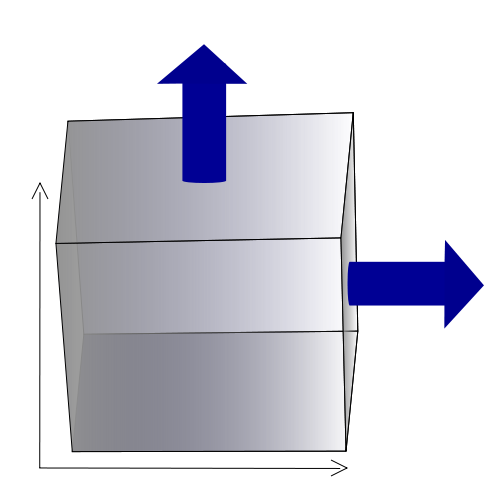
\includegraphics[width=40mm,height=40mm,keepaspectratio=true]{./Physik/Bilder/Spannung.png}
\end{center}
\end{multicols}


\subsubsection*{Schubmodul}
\index{Elastizitätslehre!Schub}
\begin{multicols}{2}{}
\begin{align*}
G&=\frac{\tau}{\varphi}
\end{align*}
\hfill

\begin{center}
 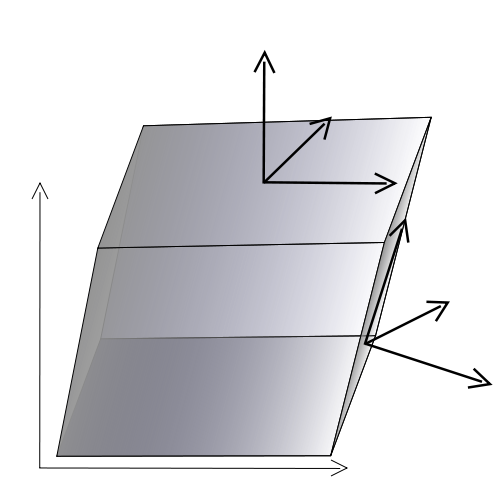
\includegraphics[width=40mm,height=40mm,keepaspectratio=true]{./Physik/Bilder/Tangentialspannung.png}
\end{center}
\end{multicols}


\subsubsection*{Drillung}
\index{Elastizitätslehre!Drill}
\begin{multicols}{2}{}
\begin{align*}
\psi&=\frac{\diff \varphi}{\diff l}=\frac{W_t}{G\cdot J_p}\tau=\frac{M_t}{G\cdot J_p}
\end{align*}
\hfill

\begin{center}
 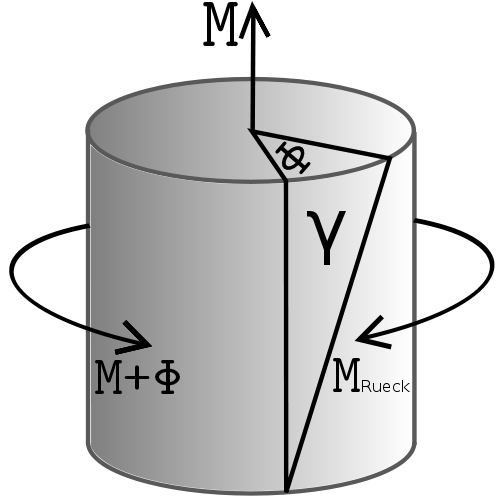
\includegraphics[width=40mm,height=40mm,keepaspectratio=true]{./Physik/Bilder/Scherbeanspruchung.png}
\end{center}
\end{multicols}


\begin{multicols}{2}{}
\subsubsection*{Flächenmoment}
\index{Elastizitätslehre!Flächenmoment}
\begin{align*}
J_p&=\int r^2\diff A=\int_\varphi\int_r r^3\diff r \diff \varphi 
\end{align*}


\subsubsection*{Verformungsarbeit}
\index{Elastizitätslehre!Verformungsarbeit}
\begin{align*}
W&=V\int \sigma(\varepsilon) \diff \varepsilon 
\end{align*}
\end{multicols}


\section{Schwingungen}
\subsection*{}%Leer hmpf\ldots!

\subsubsection*{Harmonische Schwingungen}
\begin{align*}
u(t)=A\cos(\omega t+\varphi_0)
\end{align*}


\subsection{Ungedämpfte Schwingungen}

\begin{align*}
\ddot{x}&=-\frac{k}{m}x\\
x(t)&=\hat{x}\cos(\omega_0 t+\varphi_0)\\
\dot{x}(t)&=-\hat{x}\omega\sin(\omega_0 t+\varphi_0)\\
\ddot{x}(t)&=-\hat{x}\omega^2\cos(\omega_0 t+\varphi_0)\\
\omega&=\sqrt{\frac{k}{m}}\\
f&=\frac{1}{2\pi}\sqrt{\frac{k}{m}}\\
T&=2\pi\sqrt{\frac{m}{k}}
\end{align*}

\newpage
\begin{multicols}{2}{}
\subsubsection*{Mathemetisches Pendel}
\index{Schwingungen!Mathematisches Pendel}
\begin{align*}
\ddot{\varphi}&=-\frac{g}{l}\varphi\\
\varphi(t)&=\hat{\varphi}\cos(\omega_0 t+\varphi_0)\\
\dot{\varphi}(t)&=-\hat{\varphi}\omega\sin(\omega_0 t+\varphi_0)\\
\ddot{\varphi}(t)&=-\hat{\varphi}\omega^2\cos(\omega_0 t+\varphi_0)\\
\omega&=\sqrt{\frac{g}{l}}\\
f&=\frac{1}{2\pi}\sqrt{\frac{g}{l}}\\
T&=2\pi\sqrt{\frac{l}{g}}
\end{align*}

\subsubsection*{Physikalisches Pendel}
\index{Schwingungen!Physikalisches Pendel}
\begin{align*}
\ddot{\varphi}&=-\frac{lmg}{J_A}\varphi\\
\varphi(t)&=\hat{\varphi}\cos(\omega_0 t+\varphi_0)\\
\dot{\varphi}(t)&=-\hat{\varphi}\omega\sin(\omega_0 t+\varphi_0)\\
\ddot{\varphi}(t)&=-\hat{\varphi}\omega^2\cos(\omega_0 t+\varphi_0)\\
\omega&=\sqrt{\frac{mgl}{J_A}}\\
f&=\frac{1}{2\pi}\sqrt{\frac{mgl}{J_A}}\\
T&=2\pi\sqrt{\frac{J_A}{mgl}}
\end{align*}
\end{multicols}

\begin{multicols}{2}{}
\subsubsection*{Torsionsschwingung}
\index{Schwingungen!Torsionsschwingung}
\begin{align*}
\ddot{\varphi}&=-\frac{D}{J_A}\varphi\\
\varphi(t)&=\hat{\varphi}\cos(\omega_0 t+\varphi_0)\\
\dot{\varphi}(t)&=-\hat{\varphi}\omega\sin(\omega_0 t+\varphi_0)\\
\ddot{\varphi}(t)&=-\hat{\varphi}\omega^2\cos(\omega_0 t+\varphi_0)\\
\omega&=\sqrt{\frac{D}{J_A}}\\
f&=\frac{1}{2\pi}\sqrt{\frac{D}{J_A}}\\
T&=2\pi\sqrt{\frac{J_A}{D}}
\end{align*}



\subsubsection*{Flüssigkeitspendel}
\index{Schwingungen!Flüssigkeitspendel}
\begin{align*}
\ddot{y}&=-\frac{2A\rho g}{m}y\\
\varphi(t)&=\hat{y}\cos(\omega_0 t+\varphi_0)\\
\dot{\varphi}(t)&=-\hat{y}\omega\sin(\omega_0 t+\varphi_0)\\
\ddot{\varphi}(t)&=-\hat{y}\omega^2\cos(\omega_0 t+\varphi_0)\\
\omega&=\sqrt{\frac{2A\rho g}{m}}=\sqrt{\frac{2g}{l}}\\
f&=\frac{1}{2\pi}\sqrt{\frac{2g}{l}}\\
T&=2\pi\sqrt{\frac{l}{2g}}
\end{align*}
\end{multicols}

\begin{multicols}{2}
\subsubsection*{Elektrischer Schwingkreis}
\begin{align*}
0&=L\ddot{Q}+\frac{Q}{C}\\
q(t)&=\hat{Q}\cos(\omega_0 t+\varphi_0)\\
\dot{q}(t)&=-\hat{Q}\omega\sin(\omega_0 t+\varphi_0)\\
\ddot{q}(t)&=-\hat{Q}\omega^2\cos(\omega_0 t+\varphi_0)\\
\omega&=\sqrt{\frac{1}{LC}}\\
f&=\frac{1}{2\pi}\sqrt{\frac{1}{LC}}\\
T&=2\pi\sqrt{\frac{1}{LC}}
\end{align*}
\vfill
\end{multicols}


\subsection{Gedämpfte Schwingungen}

\begin{multicols}{2}{}
\subsubsection*{Schwingungsgleichung}
\index{Schwingungen!gedämpft!Schwingungsgleichung}
\begin{align*}
m\ddot{x}=-kx+F_R
\end{align*}
\hfill

\subsubsection*{COULOMB Reibung}
\index{Schwingungen!gedämpft!COULOMB Reibung}
\begin{align*}
F_R&=-\operatorname{sgn}({\dot{x}})\mu F_N\\
0&=m\ddot{x}+kx+\operatorname{sgn}({\dot{x}})\mu F_N\\
\end{align*}
\end{multicols}


\subsubsection*{Gleitreibung}
\index{Schwingungen!gedämpft!Gleitreibung}
\begin{align*}
x(t)&=-(\hat{x}_0-\hat{x}_1)\cos(\omega t)-\hat{x}_1\qquad 0\leq t\leq \frac{T}{2}\\
x(t)&=-(\hat{x}_0-3\hat{x}_1)\cos(\omega t)+\hat{x}_1\qquad \frac{T}{2}\leq t\leq T\\
\hat{x}_1&=\frac{\mu F_N}{k}
\end{align*}


\subsubsection*{Viskosereibung}
\index{Schwingungen!gedämpft!Viskosereibung}
\begin{multicols}{2}{}
\begin{align*}
0&=m\ddot{x}+b\dot{x}+kx\\
x(t)&=\hat{x}e^{-\delta t}e^{\pm j\sqrt{\omega_0^2-\delta^2}t}\\
x(t)&=\hat{x}e^{-\delta t}e^{\pm j\omega_0\sqrt{1-D^2}t}\\
\delta&=\frac{b}{2m}\\
D&=\frac{\delta}{\omega_0}\\
D&=\frac{b}{2}\frac{1}{\sqrt{mk}}\\
\omega_0&=\sqrt{\frac{k}{m}}\\
\Lambda&=\ln\left(\frac{x(t)}{x(t+T)}\right)\\
\Lambda&=\delta T\\
\omega_D&=\sqrt{\frac{k}{m}-\left(\frac{b}{2m}\right)^2}\\
d&=2D\\
Q&=\frac{1}{d}
\end{align*}

{
\begin{align*}
x(t)&=\hat{x}e^{-\delta t}\cos(\sqrt{\omega_0^2-\delta^2}t+\varphi)\\
\end{align*}

\begin{align*}
&\text{Aperiodischer Grenzfall $\delta=\omega_0$}\\
&x(t)=\hat{x}e^{-\delta t}(1-\delta t)
\end{align*}

\begin{align*}
&\text{Kriechfall $\delta>\omega_0$}\\
&x(t)=\hat{x}e^{-\delta t}e^{\pm j\sqrt{\omega_0^2-\delta^2}t}
\end{align*}
}
\hfill

\end{multicols}

		\chapter{Fluiddynamik}
		\begin{multicols}{2}
\begin{quote}
  Premature optimization\\is the root of all evil.\\- D. Knuth
\end{quote}
\vfill
\begin{quote}
 On the other hand,\\we cannot ignore efficiency.\\- Jon Bentley
\end{quote}
\vfill
\end{multicols}

\section{Ohne Reibung}
\index{Fluiddynamik!Ohne Reibung}
\begin{multicols}{3}
\subsubsection*{Statischer Druck}
\begin{align*}
p&=\frac{\diff F_N}{\diff A}
\end{align*}

\subsubsection*{Dynamischer Druck}
\begin{align*}
p&=\frac{1}{2}\rho v^2
\end{align*}

\subsubsection*{Schweredruck}
\begin{align*}
p&=\frac{\rho V g}{A}\\
&=h\rho g
\end{align*}
\end{multicols}

\begin{multicols}{2}
\subsubsection*{Volumenstrom}
\begin{align*}
\dot{V}&=v A\\
&=\iint_A \vec{v} \diff\vec{ A}\\
&=\frac{\diff V}{\diff t}\\
&=Q
\end{align*}

\subsubsection*{Massenstrom}
\begin{align*}
\dot{m}&=jA\\
&=\iint_A \vec{j} \diff\vec{A}\\
&=\frac{\diff m}{\diff t}
\end{align*}
\end{multicols}

\begin{multicols}{2}
\subsubsection*{Auftrieb}
\begin{align*}
\vec{F_A}&=-\rho_V \vec{g} V\\
&=-\frac{\rho_V}{\rho_M}\vec{F_G}
\end{align*}

\subsubsection*{Kontinuitätsgleichung}
\begin{alignat*}{2}
\left.\dot{m}\right|_1&=\left.\dot{m}\right|_2 & \quad \left.\dot{V}\right|_1&=\left.\dot{V}\right|_2\\
v_1A_1&=v_2A_2 & \rho_1&=\rho_2
\end{alignat*}
\end{multicols}

\begin{multicols}{2}{}
\subsubsection*{Kompressibilität}
\begin{align*}
\kappa&=\frac{\Delta V}{\Delta p V}
\end{align*}


\subsubsection*{Volumenausdehnungskoeffezient}
\begin{align*}
\frac{\Delta V}{V}&= \gamma \Delta T
\end{align*}


\subsubsection*{Barometrische Höhenformel}
\begin{align*}
p&=p_0 e^{-Ch}\\
C&=\frac{\rho_0 g}{p_0}
\end{align*}


\subsubsection*{Bernoulli Gleichung}
\begin{align*}
p+\frac{1}{2}\rho v^2+ \rho g h= \text{const}
\end{align*}
\end{multicols}


\section{Laminare Reibung}
\index{Fluiddynamik!Laminare Reibung}
\begin{multicols}{2}{}
\subsubsection*{Newtonsches Reibungsgesetz}
\begin{align*}
F_R&=\eta A \frac{\diff v}{\diff x}
\end{align*}


\subsubsection*{Laminare Strömung (Rohr)}
\begin{align*}
v(r)&=\frac{p}{4\eta l}\left(R^2-r^2\right)\\
p&=\frac{4\eta l}{R^2}v(0)\\
\dot{V}&=\frac{\pi R^4}{8\eta l}p
\end{align*}


\subsubsection*{Umströmung (Kugel)}
\begin{align*}
F_R=6\pi\eta r v
\end{align*}



\subsubsection*{Bernoulligleichung mit Reibung}
\begin{align*}
&p_1+\frac{1}{2}\rho v_1^2+ \rho g h_1 \\
=&p_2+\frac{1}{2}\rho v_2^2+ \rho g h_2+\Delta p
\end{align*}


\subsubsection*{Reynoldszahl}
\begin{align*}
Re&=\frac{L\rho v}{\eta}\\
Re&>Re_{krit}\\
&\text{Strömung wird Turbulent}
\end{align*}
\end{multicols}


		\chapter{Gravitation}
		 \begin{quote}
  The year is 787!\\A.D.?\\- Monty Python
 \end{quote}

\begin{multicols}{2}{}
\subsubsection*{Gravitationskraft}
\begin{align*}
\vec{F}_{g,2}&=-G\frac{m_1m_2}{r_{12}^2}\vec{e}_r\\
\vec{F}_g&=\vec{E}_g\cdot m=\vec{g}m
\end{align*}
\hfill

\subsubsection*{Gravitationspotential}
\begin{align*}
\phi&=-G\frac{M}{r}\\
\vec{E}_g&=\grad\phi
\end{align*}
\hfill
\end{multicols}

\begin{multicols}{2}{}
\subsubsection*{Arbeit}
\begin{align*}
W_{12}&=-\int_{\vec{r}_1}^{\vec{r}_2}\vec{F}_g\circ\diff\vec{r}\\
&=GmM\left(\frac{1}{r_1}-\frac{1}{r_2}\right)
\end{align*}

\subsubsection*{Planetenbahnen}
\begin{align*}
\left(\frac{a}{a_E}\right)^3=\left(\frac{T}{T_E}\right)^2
\end{align*}
\hfill
\end{multicols}


		\chapter{Elektrostatik}
		 \begin{quote}
  Don't interrupt me\\while I'm interrupting.\\- Winston S. Churchill
 \end{quote}

\begin{multicols}{2}{}
\subsubsection{Ladung}
\begin{align*}
Q&=n\cdot e_0\\
&=CU\\
&=\int i \diff t
\end{align*}

\subsubsection{Punktladungen}
\begin{align*}
\vec{E}(\vec{r})&=\sum_{i=1}^{N}\vec{E}_i{\vec{r}_i}
\end{align*}
\vspace{15mm}
\end{multicols}

\begin{multicols}{2}{}
\subsubsection{COULOMB Gesetz}
\begin{align*}
\vec{F}_{12}&=\frac{1}{4\pi\epsilon}\frac{Q_1Q_2}{r^2}\vec{r_12}\\
&=\vec{E}Q\\
\vec{E}&=\frac{1}{4\pi\epsilon}\frac{Q}{r^2}\vec{r}\\
&=-\grad\varphi\\
&=-\left(\frac{\partial \varphi}{\partial x}\vec{e}_x+\frac{\partial \varphi}{\partial y}\vec{e}_y+\frac{\partial \varphi}{\partial z}\vec{e}_z\right)
\end{align*}

\subsubsection{Spannung}
\begin{align*}
U_{AB}=&\frac{W_{AB}}{Q}\\
=&\int_A^B\vec{E}\circ\diff\vec{s}\\
=&\oint_s\vec{E}\circ\diff\vec{s}=0\\
=&\varphi_A-\varphi_B\\
=&-\int_\infty^A\vec{E}\circ\diff\vec{s}\\
&-\left(-\int_\infty^B\vec{E}\circ\diff\vec{s}\right)
\end{align*}
\vfill
\end{multicols}

\newpage
\begin{multicols}{2}{}
\subsubsection{El- / Verschiebungsfluß}
\begin{align*}
\psi&=\int_A\vec{E}\circ\diff\vec{A}\\
\psi&=\oint_A\vec{E}\circ\diff\vec{A}=\frac{Q}{\epsilon}\\
\end{align*}

\subsubsection{Flußdichte}
\begin{align*}
\vec{D}&=\frac{\diff Q}{\diff A}\vec{e}_A\\
\vec{D}&=\epsilon\vec{E}\\
Q&=\oint_AD\diff A
\end{align*}
\end{multicols}

\subsubsection{Kapazität}
\begin{align*}
Q&=CU
\end{align*}

\begin{multicols}{2}{}
\subsubsection{OHMsches Gesetz}
\begin{align*}
I &=\oint_A\vec{j}\circ\diff\vec{A}\\
  &=\oint_A \kappa\vec{E}\circ\diff\vec{A}\\
  &=\underbrace{\kappa E\cdot 4\pi r^2}_{\text{Kugel}}
\end{align*}
\vspace{20mm}

\subsubsection{Arbeit im elektrischem Feld}
\begin{align*}
w&=\frac{1}{2}\vec{E}\circ\vec{D}\\
W&=\int_Vw\diff V\\
 &=-Q\int_A^B\vec{E}\circ\diff\vec{s}\\
 &=\int_U Q\diff U\\
 &= \int_U CU \diff U\\
 &=\frac{1}{2}CU^2
\end{align*}
\end{multicols}


		\chapter{Thermodynamik}
		\begin{multicols}{2}
\section{Wärmedehnung}
\begin{align*}
\rho(T)&=\rho_0(1-\beta(T-T_0))\\
V(T)&=V_0(1+\gamma(T-T_0))\\
l(T)&=l_0(1+\alpha(T-T_0))\\
\gamma&\approx 3\cdot \alpha\\
\gamma&\approx \beta
\end{align*}

\section{Wärme}
\begin{align*}
\Delta Q&=c\cdot m(T-T_0)\\
\Delta Q&=C(T-T_0)\\
\Delta Q&=\int_{T_0}^T c\cdot m \diff T\\
\Delta Q&=c_{mol}\cdot n(T-T_0)
\end{align*}

\section{Mischtemperatur}
\begin{align*}
T_m&=\frac{\sum_{i=1}^n T_i m_i c_i}{\sum_{i=1}^n m_i c_i} \\
\dot{Q}&\text{Ist durch einen mehrschichtiges}\\
&\text{stationäres System Konstant}
\end{align*}

\section{Wärmeleitung}
\begin{align*}
\dot{Q}&=\frac{\diff Q}{\diff t}=\varPhi=P\\
\vec{\dot{q}}&=\frac{\dot{Q}}{A}\cdot\vec{e_A}\\
\vec{\dot{q}}&=-\lambda\grad{T}\\
\vec{\dot{q}}&=\frac{\lambda}{s}\left(T_A-T_B\right)\cdot\vec{e_s}\\
\dot{q}&=\frac{1}{\sum_{i=1}^n\frac{s_i}{\lambda_i}}\cdot\left(T_A-T_B\right)
\end{align*}

\section{Wärmekonvektion}
\begin{align*}
\dot{q}&=\alpha\left(T_A-T_B\right)\\
\dot{q}&=\frac{1}{\sum_{i=1}^n\frac{1}{\alpha_i}}\cdot\left(T_A-T_B\right)
\end{align*}
\vfill
\end{multicols}

\section{Wärmewiderstand}

\[R_{th}=\frac{T_A-T_B}{\dot{q}\cdot A}=\frac{s}{\lambda A}=\frac{1}{\alpha A}=\sum_{i=1}^n R_{i}\]

\subsection{Wärmeübertragung}
\begin{align*}
k&=\frac{1}{\sum_{i=1}^n\frac{s_i}{\lambda_i}+\sum_{i=1}^n\frac{1}{\alpha_i}+\sum_{i=1}^n R_{i}}\\
\dot{q}&=\frac{1}{\sum_{i=1}^n\frac{s_i}{\lambda_i}+\sum_{i=1}^n\frac{1}{\alpha_i}+\sum_{i=1}^n R_{i}}\cdot\left(T_A-T_B\right)\\
\dot{q}&=k\cdot\left(T_A-T_B\right)
\end{align*}

\subsection{Wärmestrahlung}
\begin{align*}
\alpha&=\varepsilon\\
1&=\alpha+\tau+\vartheta\\
\dot{Q}&=\varepsilon A \sigma T^4\\
\dot{Q}_{AB}&=C_{AB}A_A\left(T_A^4-T_B^4\right)\\
C_{AB}&=\varepsilon_{AB}\sigma=\frac{\sigma}{\frac{1}{\varepsilon_A}+\frac{1}{\varepsilon_B}-1}=\frac{1}{\frac{1}{\sigma_A}+\frac{1}{\sigma_B}-\frac{1}{\sigma}}&&\text{Parallel}\\
C_{AB}&=\frac{\sigma}{\frac{1}{\varepsilon_A}+\frac{A_A}{A_B}\left(\frac{1}{\varepsilon_B}-1\right)}&&\text{$A_A$ von $A_B$ umschlossen}\\
C_{AB}&\approx\varepsilon_A\sigma&&\text{parallel ($A_A\ll A_B$)}
\end{align*}

\subsection{Zustandsänderung des idealen Gases}
Teilchen stehen nicht in Wechselwirkung, besitzen kein Volumen \\ und es kommt zu keinem Phasenübergang

\newpage
\begin{multicols}{2}
\subsubsection*{Energie}
\begin{align*}
U_{12}&=Q_{12}+W_{12}\\
&\text{Nur Isobar:}\\
\diff H&=c_pm\diff T=U+p\diff V\\
\diff S&=\frac{\diff Q}{T}
\end{align*}
\vfill

\subsubsection*{Zustandsgleichung}
\begin{align*}
\frac{pV}{T}&=\text{const}\\
pV&=NkT=mR_sT=nRT\\
R_s&=\frac{nR}{m}\\
R_s&=c_p-c_v
\end{align*}
\end{multicols}

\begin{multicols}{2}
\subsubsection*{Isotherm}
\begin{align*}
pV&=\text{const}\\
T&=\text{const}\\
U_{12}&=0\\
U_{12}&=Q_{12}+ W_{12}\\
Q_{12}&=-W_{12}\\
W_{12}&=p_1V_1\ln{\frac{V_2}{V_1}}\\
W_{12}&=p_1V_1\ln{\frac{p_1}{p_2}}\\
S_{12}&=mc_p\ln{\frac{V_2}{V_1}}+mc_V\ln{\frac{p_2}{p_1}}
\end{align*}

\subsubsection*{Isobar}
\begin{align*}
\frac{V}{T}&=\text{const}\\
p&=\text{const}\\
Q_{12}&=mc_p\left(T_2-T_1\right)\\
W_{12}&=-p\left(V_2-V_1\right)\\
U_{12}&=Q_{12}+ W_{12}\\
S_{12}&=mc_p\ln{\frac{V_2}{V_1}}
\end{align*}

\subsubsection*{Isochor}
\begin{align*}
\frac{p}{T}&=\text{const}\\
V&=\text{const}\\
Q_{12}&=mc_v\left(T_2-T_1\right)\\
W_{12}&=0\\
U_{12}&=Q_{12}\\
S_{12}&=mc_v\ln{\frac{p_2}{p_1}}
\end{align*}

\subsubsection*{Adiabat}
\begin{align*}
pV^\kappa&=\text{const}\\
Q&=\text{const}\\
\kappa&=\frac{c_p}{c_V}\\
\frac{T_2}{T_1}&=\left(\frac{V_2}{V_1}\right)^{1-\kappa}=\left(\frac{p_2}{p_1}\right)^{\frac{\kappa-1}{\kappa}}\\
Q_{12}&=0\\
W_{12}&=mc_v\left(T_2-T_1\right)\\
W_{12}&=\frac{RT_1}{\kappa-1}\left(\left(\frac{V_2}{V_1}\right)^{1-\kappa}-1\right)\\
U_{12}&=W_{12}\\
S_{12}&=0;
\end{align*}
\end{multicols}

\begin{multicols}{2}
\subsubsection*{Kreisprozess}
\begin{align*}
\oint \diff U&=0\\
\oint \diff U&= \oint \diff Q +\oint \diff W\\
&\text{Revesiebel:}
\oint \diff S&=0\\
&\text{Irrevesiebel}
\oint \diff S&>0\\
\end{align*}

\subsubsection*{Carnot-Prozeß}
\begin{align*}
\eta_C&=\frac{W_{ab}}{Q_{zu}}\\
\eta_C&=\frac{Q_{zu}-Q_{AB}}{Q_{zu}}\\
\eta_C&=\frac{T_h-T_n}{T_n}
\end{align*}
\vfill
\end{multicols}

		\chapter{Optik}
		\begin{quote}
The path taken between two points by a ray of light\\is the path that can be traversed in the least time.\\- Pierre de Fermat
\end{quote}  

\begin{multicols}{2}
\section{Brechung}
\begin{align*}
\frac{\sin{\varepsilon_1}}{\sin{\varepsilon_2}}&=\frac{n_2}{n_1}=\frac{c_1}{c_2}\\
\varepsilon_2&=\arcsin{\frac{\sin{\varepsilon_1}\cdot n_1}{n_2}}
\end{align*}

\section{Totalreflexion}
\begin{align*}
\sin{\varepsilon_g}&=\frac{n_2}{n_1}
\end{align*}
\end{multicols}

Totalreflexion tritt nur auf, wenn der Lichtstrahl von einen dichteren \\ in ein optisch dünneren Stoff übergeht.

\section{Hohlspiegel}
\begin{multicols}{2}
\begin{center}
 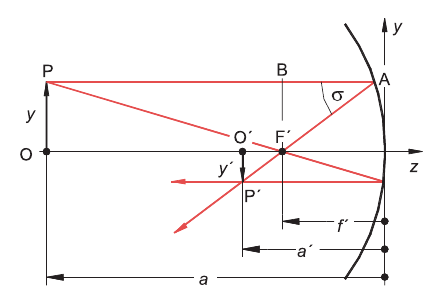
\includegraphics[width=60mm,keepaspectratio=true]{./Physik/Bilder/Hohlspiegel.png}
\end{center}

\begin{align*}
\frac{1}{f'}&=\frac{1}{a}+\frac{1}{a'}\\
f'&=\frac{r}{2}\\
\beta'&=\frac{y'}{y}\\
\beta'&=-\frac{a'}{a}
\end{align*}
\end{multicols}

\section{Linse}
\begin{multicols}{2}
\begin{center}
 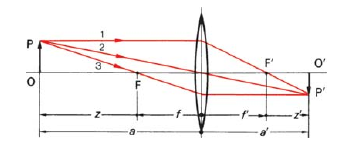
\includegraphics[width=60mm,keepaspectratio=true]{./Physik/Bilder/Linse.png}
\end{center}
\begin{align*}
\frac{1}{f'}&=\frac{1}{a'}-\frac{1}{a}\\
\frac{1}{f}&=\frac{1}{a'}+\frac{1}{a}\\
f&=\frac{a\cdot a'}{a+a'}=-f'\\
a'&=\frac{af'}{a+f'}\\
\beta'&=\frac{f'}{a+f'}\\
\beta'&=\frac{y'}{y}\\
D'&=\frac{1}{f'}=\left(n_L-1\right)\cdot\left(\frac{1}{r_1}-\frac{1}{r_2}\right)
\end{align*}
\end{multicols}

\begin{center}
 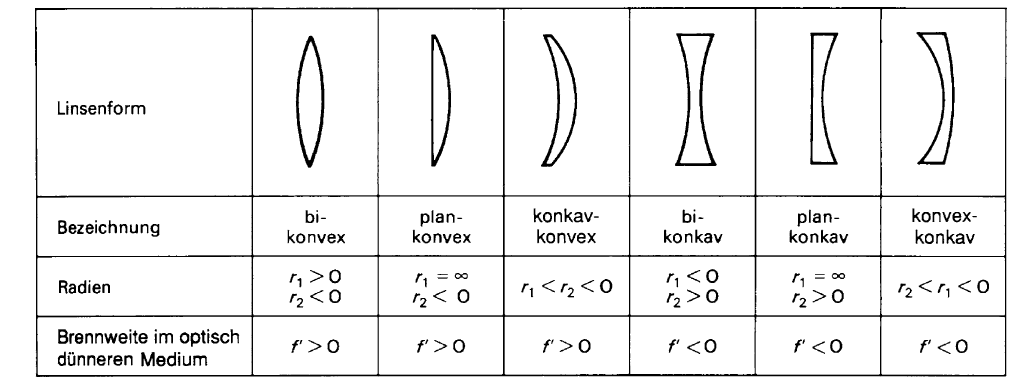
\includegraphics[width=129mm,keepaspectratio=true]{./Physik/Bilder/Beispiele-Linsen.png}
\end{center}

\newpage
\section{Lichtwellenleiter}
\begin{multicols}{2}
\begin{center}
 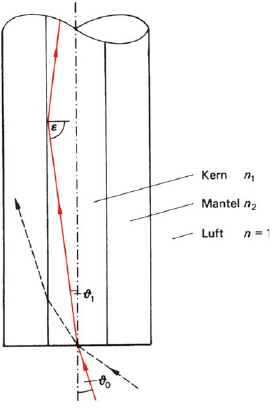
\includegraphics[width=50mm,keepaspectratio=true]{./Physik/Bilder/Lichtwellenleiter.png}
\end{center}

\subsection*{Totalreflexion (Grenzwinkel)}
\[n_1\sin\left(90^\circ-\vartheta_1\right)=n_2 \Longrightarrow \cos\vartheta_1=\frac{n_2}{n_1}\]

\subsection*{numerische Apertur}
\begin{align*}
 A_{WL}&=n_0 \sin\vartheta_0=n_1\sqrt{1-\cos^2\vartheta_1}\\&=n_1\sqrt{1-\left(\frac{n_2}{n_1}\right)^2}\\&=\sqrt{n_1^2-n_2^2}\\&=\sqrt{n_{Kern}^2-n_{Mantel}^2}
\end{align*}
\end{multicols}


	\part{Elektrotechnik}

		\chapter{Gleichstromtechnik}
		\section{Grundgrößen}

\subsubsection{Elementarladung}
\begin{multicols}{2}{}
\begin{align*}
e\approx 1,6\cdot 10^{-19}C
\end{align*}
\hfill

\begin{align*}
\left[Q\right]&=1C=1As\\
Q&=n\cdot e
\end{align*}
\end{multicols}


\begin{multicols}{2}{}
\subsubsection{Strom}
\begin{align*}
\left[I\right]&=1A\\
i(t)&=\frac{\diff Q}{\diff t}
\end{align*}

\subsubsection{Stromdichte}
\begin{align*}
\left[J\right]&=1\frac{A}{mm^2}\\
\vec{J}&=\frac{I}{\vec{A}}
\end{align*}
\end{multicols}


\begin{multicols}{2}{}
\subsubsection{Potential}
\begin{align*}
\left[\varphi\right]&=1V=1\frac{Nm}{As}=1\frac{kgm^2}{As^3}\\
\varphi&=\frac{W}{Q}
\end{align*}

\subsubsection{Spannung}
\begin{align*}
\left[U\right]&=1V\\
U_{AB}&=\varphi_a-\varphi_b
\end{align*}
\hfill
\end{multicols}


\subsubsection{Widerstand und Leitwert}

\begin{multicols}{2}{}
\begin{align*}
\left[R\right]&=1\Omega=1\frac{V}{A}\\
R&=\frac{U}{I}\\
&=\rho\frac{l}{A}=\frac{1}{\kappa}\frac{l}{A}
\end{align*}
\hfill

\begin{align*}
\left[G\right]&=1S=1\frac{A}{V}\\
G&=\frac{I}{U}\\
&=\frac{1}{R}\\
&=\kappa\frac{A}{l}=\frac{1}{\rho}\frac{A}{l}
\end{align*}
\end{multicols}


\subsubsection{Temperaturabhängigkeit}
\begin{align*}
R_2=R_1\cdot\left(1+\alpha\left(\vartheta_2-\vartheta_1\right)+\beta\left(\vartheta_2-\vartheta_1\right)^2\right)
\end{align*}


\begin{multicols}{2}{}
\subsubsection{Leistung}
\begin{align*}
\left[P\right]&=1W=1VA\\
P&=u(t)\cdot i(t)
\end{align*}

\subsubsection{Leistung im Mittel}
\begin{align*}
P&=\frac{1}{T}\int_0^T u(t)\cdot i(t)\diff t 
\end{align*}
\hfill
\end{multicols}


\section{Lineare Quellen}


\begin{multicols}{2}{}
\subsubsection{Spannungsquelle}
\begin{align*}
U&=U_q-R_i\cdot I\\
I_K&=\frac{U_q}{R_i}
\end{align*}

\subsubsection{Stromquelle}
\begin{align*}
I&=I_q-\frac{U}{R_i}\\
U_l&=I_q\cdot R_i
\end{align*}
\end{multicols}


\section{Kirchhoffsche Gesetze}


\begin{multicols}{2}{}
\subsubsection{Knotenpunktsatz}
\begin{align*}
\sum_{i=1}^n I_i=0
\end{align*}

\subsubsection{Maschensatz}
\begin{align*}
\sum_{i=1}^n U_i=0
\end{align*}
\end{multicols}


		\chapter{Wechselstromtechnik}
		\section{Definitionen}

\subsection{periodische zeitabhängige Größen}
Allgemein \(x\left(t\right) \xrightarrow{}\) speziell \(u\left(t\right); i\left(t\right); q\left(t\right); \dots\) \\
es gillt \(x\left(t\right) = x\left(t + n \cdot T\right) ; \left(n \in \N^* \right) \)

\subsection{Wechselgrößen}
Allgemein \(x_{\sim} \left(t\right)\); periodisch sich ändernde Größe, deren Gleichanteil bzw. 
zeitlich linearer Mittelwert gleich Null ist. \\ \vspace{0mm} \\
Nachweis: \[\int_{t1}^{t1 + n \cdot T} x_{\sim} \left(t\right)dt = 0 \; ; \; \left(n \in \N^* \right) \;
; \; t1 \; \text{beliebiger Zeitwert}\]

\subsection{Mischgrößen}
Sind periodisch, Ihr Gleichanteil \(\overline{x}\) bzw. zeitlich linearer Mittelwert \\
jedoch ist ungleich Null. 
\begin{align*}
\text{Mischgröße} &= \text{Wechselgröße + Gleichanteil} \\
x\left(t\right) &= x_{\sim}\left(t\right) + \overline{x} \\
&= \text{gleichanteilbehaftete Wechselgröße}
\end{align*}

\newpage
\section{Anteile und Formfaktoren}

\begin{multicols}{2}{}
\subsection{Gleichanteil}
\[ \overline{x} = \frac{1}{n \cdot T} \cdot \int_{t_{1}}^{t_{1} + n \cdot T} x \left( t \right) dt \]
\hfill

\subsection{Gleichrichtwert}
\[ \left| \overline{x} \right| = \frac{1}{n \cdot T} \cdot 
\int_{t_{1}}^{t_{1} + n \cdot T} \left| x \right| \left( t \right) dt\]
\hfill
\end{multicols}

\(n \in \N^* \;; \; t1 \; \text{beliebiger Zeitwert} \;; \; 
\left[|\overline{x} \right|] = \left[ x\left( t \right) \right] \)




		\chapter{Signal- und Systemtheorie}
		\section{Einfache Impulse}
\subsection*{Rechteckimpuls/ -funktion \texorpdfstring{$rect_T\left(t\right)$}{}}
\begin{multicols}{2}
\begin{equation*}
x\left(t\right) = X_0 \cdot rect_T\left(t\right) 
\end{equation*}

\begin{itemize}
 \item T: Rechteckimpulsbreite \(> 0\)
 \item an den Sprungstellen nimmt der Impuls die Hälfte des max. Wertes an
\end{itemize}

\begin{center}
 % Graphic for TeX using PGF
% Title: /home/Befedo/Documents/eclipse.workspace/Formelsammlung/Elektrotechnik/Bilder/rect.dia
% Creator: Dia v0.97
% CreationDate: Tue Jan  3 07:53:56 2012
% For: Befedo
% \usepackage{tikz}
% The following commands are not supported in PSTricks at present
% We define them conditionally, so when they are implemented,
% this pgf file will use them.
\ifx\du\undefined
  \newlength{\du}
\fi
\setlength{\du}{15\unitlength}
\begin{tikzpicture}
\pgftransformxscale{0.567523}
\pgftransformyscale{-0.567523}
\definecolor{dialinecolor}{rgb}{0.000000, 0.000000, 0.000000}
\pgfsetstrokecolor{dialinecolor}
\definecolor{dialinecolor}{rgb}{1.000000, 1.000000, 1.000000}
\pgfsetfillcolor{dialinecolor}
\pgfsetlinewidth{0.100000\du}
\pgfsetdash{}{0pt}
\pgfsetdash{}{0pt}
\pgfsetbuttcap
{
\definecolor{dialinecolor}{rgb}{0.000000, 0.000000, 0.000000}
\pgfsetfillcolor{dialinecolor}
% was here!!!
\pgfsetarrowsend{stealth}
\definecolor{dialinecolor}{rgb}{0.000000, 0.000000, 0.000000}
\pgfsetstrokecolor{dialinecolor}
\draw (0.000000\du,10.000000\du)--(16.000000\du,10.000000\du);
}
\pgfsetlinewidth{0.100000\du}
\pgfsetdash{}{0pt}
\pgfsetdash{}{0pt}
\pgfsetbuttcap
{
\definecolor{dialinecolor}{rgb}{0.000000, 0.000000, 0.000000}
\pgfsetfillcolor{dialinecolor}
% was here!!!
\pgfsetarrowsend{stealth}
\definecolor{dialinecolor}{rgb}{0.000000, 0.000000, 0.000000}
\pgfsetstrokecolor{dialinecolor}
\draw (8.000000\du,10.000000\du)--(8.000000\du,1.000000\du);
}
\pgfsetlinewidth{0.100000\du}
\pgfsetdash{}{0pt}
\pgfsetdash{}{0pt}
\pgfsetmiterjoin
\pgfsetbuttcap
{
\definecolor{dialinecolor}{rgb}{1.000000, 0.000000, 0.000000}
\pgfsetfillcolor{dialinecolor}
% was here!!!
{\pgfsetcornersarced{\pgfpoint{0.000000\du}{0.000000\du}}\definecolor{dialinecolor}{rgb}{1.000000, 0.000000, 0.000000}
\pgfsetstrokecolor{dialinecolor}
\draw (0.000000\du,10.000000\du)--(5.000000\du,10.000000\du)--(5.000000\du,5.000000\du)--(11.000000\du,5.000000\du)--(11.000000\du,10.000000\du)--(15.000000\du,10.000000\du);
}}
\pgfsetlinewidth{0.100000\du}
\pgfsetdash{}{0pt}
\pgfsetdash{}{0pt}
\pgfsetbuttcap
{
\definecolor{dialinecolor}{rgb}{0.000000, 0.000000, 0.000000}
\pgfsetfillcolor{dialinecolor}
% was here!!!
\definecolor{dialinecolor}{rgb}{0.000000, 0.000000, 0.000000}
\pgfsetstrokecolor{dialinecolor}
\draw (7.500000\du,5.500000\du)--(8.500000\du,4.500000\du);
}
\pgfsetlinewidth{0.100000\du}
\pgfsetdash{}{0pt}
\pgfsetdash{}{0pt}
\pgfsetbuttcap
{
\definecolor{dialinecolor}{rgb}{0.000000, 0.000000, 0.000000}
\pgfsetfillcolor{dialinecolor}
% was here!!!
\definecolor{dialinecolor}{rgb}{0.000000, 0.000000, 0.000000}
\pgfsetstrokecolor{dialinecolor}
\draw (5.000000\du,9.500000\du)--(5.000000\du,10.500000\du);
}
\pgfsetlinewidth{0.100000\du}
\pgfsetdash{}{0pt}
\pgfsetdash{}{0pt}
\pgfsetbuttcap
{
\definecolor{dialinecolor}{rgb}{0.000000, 0.000000, 0.000000}
\pgfsetfillcolor{dialinecolor}
% was here!!!
\definecolor{dialinecolor}{rgb}{0.000000, 0.000000, 0.000000}
\pgfsetstrokecolor{dialinecolor}
\draw (11.000000\du,9.500000\du)--(11.000000\du,10.500000\du);
}
% setfont left to latex
\definecolor{dialinecolor}{rgb}{0.000000, 0.000000, 0.000000}
\pgfsetstrokecolor{dialinecolor}
\node[anchor=east] at (5.500000\du,11.000000\du){-T/2};
% setfont left to latex
\definecolor{dialinecolor}{rgb}{0.000000, 0.000000, 0.000000}
\pgfsetstrokecolor{dialinecolor}
\node[anchor=west] at (10.500000\du,11.000000\du){T/2};
% setfont left to latex
\definecolor{dialinecolor}{rgb}{0.000000, 0.000000, 0.000000}
\pgfsetstrokecolor{dialinecolor}
\node[anchor=west] at (8.500000\du,4.500000\du){};
% setfont left to latex
\definecolor{dialinecolor}{rgb}{0.000000, 0.000000, 0.000000}
\pgfsetstrokecolor{dialinecolor}
\node[anchor=west] at (8.500000\du,4.500000\du){X0};
\end{tikzpicture}

\end{center}

\end{multicols}

\subsection*{Dreiecksimpuls/ -funktion \texorpdfstring{$\Lambda_T\left(t\right)$}{}}
\begin{multicols}{2}
 \begin{align*}
x\left(t\right) &= X_0 \cdot \Lambda_T\left(t\right) \\
\Lambda_T\left(t\right) &=\begin{cases}
1-\left|t/T\right| \text{ für } \left|t\right| < T\\
0 \text{ für } \left|t\right| > T
\end{cases}
\end{align*}

\begin{itemize}
 \item T: Dauer einer ansteigenden / abfallenden Flanke
\end{itemize}

\begin{center}
 % Graphic for TeX using PGF
% Title: /home/Befedo/Documents/eclipse.workspace/Formelsammlung/Elektrotechnik/Bilder/lambda.dia
% Creator: Dia v0.97
% CreationDate: Tue Jan  3 08:05:58 2012
% For: Befedo
% \usepackage{tikz}
% The following commands are not supported in PSTricks at present
% We define them conditionally, so when they are implemented,
% this pgf file will use them.
\ifx\du\undefined
  \newlength{\du}
\fi
\setlength{\du}{15\unitlength}
\begin{tikzpicture}
\pgftransformxscale{0.567523}
\pgftransformyscale{-0.567523}
\definecolor{dialinecolor}{rgb}{0.000000, 0.000000, 0.000000}
\pgfsetstrokecolor{dialinecolor}
\definecolor{dialinecolor}{rgb}{1.000000, 1.000000, 1.000000}
\pgfsetfillcolor{dialinecolor}
\pgfsetlinewidth{0.100000\du}
\pgfsetdash{}{0pt}
\pgfsetdash{}{0pt}
\pgfsetbuttcap
{
\definecolor{dialinecolor}{rgb}{0.000000, 0.000000, 0.000000}
\pgfsetfillcolor{dialinecolor}
% was here!!!
\pgfsetarrowsend{stealth}
\definecolor{dialinecolor}{rgb}{0.000000, 0.000000, 0.000000}
\pgfsetstrokecolor{dialinecolor}
\draw (8.000000\du,10.000000\du)--(8.000000\du,1.000000\du);
}
\pgfsetlinewidth{0.100000\du}
\pgfsetdash{}{0pt}
\pgfsetdash{}{0pt}
\pgfsetmiterjoin
\pgfsetbuttcap
{
\definecolor{dialinecolor}{rgb}{1.000000, 0.000000, 0.000000}
\pgfsetfillcolor{dialinecolor}
% was here!!!
{\pgfsetcornersarced{\pgfpoint{0.000000\du}{0.000000\du}}\definecolor{dialinecolor}{rgb}{1.000000, 0.000000, 0.000000}
\pgfsetstrokecolor{dialinecolor}
\draw (0.000000\du,10.000000\du)--(5.000000\du,10.000000\du)--(8.000000\du,5.000000\du)--(11.000000\du,10.000000\du)--(15.000000\du,10.000000\du);
}}
% setfont left to latex
\definecolor{dialinecolor}{rgb}{0.000000, 0.000000, 0.000000}
\pgfsetstrokecolor{dialinecolor}
\node[anchor=west] at (8.500000\du,4.500000\du){};
\pgfsetlinewidth{0.100000\du}
\pgfsetdash{}{0pt}
\pgfsetdash{}{0pt}
\pgfsetbuttcap
{
\definecolor{dialinecolor}{rgb}{0.000000, 0.000000, 0.000000}
\pgfsetfillcolor{dialinecolor}
% was here!!!
\definecolor{dialinecolor}{rgb}{0.000000, 0.000000, 0.000000}
\pgfsetstrokecolor{dialinecolor}
\draw (5.000000\du,9.500000\du)--(5.000000\du,10.500000\du);
}
\pgfsetlinewidth{0.100000\du}
\pgfsetdash{}{0pt}
\pgfsetdash{}{0pt}
\pgfsetbuttcap
{
\definecolor{dialinecolor}{rgb}{0.000000, 0.000000, 0.000000}
\pgfsetfillcolor{dialinecolor}
% was here!!!
\definecolor{dialinecolor}{rgb}{0.000000, 0.000000, 0.000000}
\pgfsetstrokecolor{dialinecolor}
\draw (11.000000\du,9.500000\du)--(11.000000\du,10.500000\du);
}
\pgfsetlinewidth{0.100000\du}
\pgfsetdash{}{0pt}
\pgfsetdash{}{0pt}
\pgfsetbuttcap
{
\definecolor{dialinecolor}{rgb}{0.000000, 0.000000, 0.000000}
\pgfsetfillcolor{dialinecolor}
% was here!!!
\pgfsetarrowsend{stealth}
\definecolor{dialinecolor}{rgb}{0.000000, 0.000000, 0.000000}
\pgfsetstrokecolor{dialinecolor}
\draw (0.000000\du,10.000000\du)--(16.000000\du,10.000000\du);
}
% setfont left to latex
\definecolor{dialinecolor}{rgb}{0.000000, 0.000000, 0.000000}
\pgfsetstrokecolor{dialinecolor}
\node[anchor=east] at (5.000000\du,11.000000\du){-T};
% setfont left to latex
\definecolor{dialinecolor}{rgb}{0.000000, 0.000000, 0.000000}
\pgfsetstrokecolor{dialinecolor}
\node[anchor=west] at (11.000000\du,11.000000\du){T};
\pgfsetlinewidth{0.100000\du}
\pgfsetdash{}{0pt}
\pgfsetdash{}{0pt}
\pgfsetbuttcap
{
\definecolor{dialinecolor}{rgb}{0.000000, 0.000000, 0.000000}
\pgfsetfillcolor{dialinecolor}
% was here!!!
\definecolor{dialinecolor}{rgb}{0.000000, 0.000000, 0.000000}
\pgfsetstrokecolor{dialinecolor}
\draw (7.500000\du,5.500000\du)--(8.500000\du,4.500000\du);
}
% setfont left to latex
\definecolor{dialinecolor}{rgb}{0.000000, 0.000000, 0.000000}
\pgfsetstrokecolor{dialinecolor}
\node[anchor=west] at (8.500000\du,4.500000\du){1};
\end{tikzpicture}

\end{center}

\end{multicols}

\section{Elementare Operationen auf zeitliche Verläufe}
\subsection*{Beeinflußung der Ordinate}

\begin{multicols}{2}
 \subsubsection*{Signaloffset \texorpdfstring{$X_{OFFS}$}{}}
  \begin{equation*}
   x_{neu}\left(t\right) = x_{alt}\left(t\right) + X_{OFFS} 
  \end{equation*}
\vfill
  \begin{center}
  % Graphic for TeX using PGF
% Title: /home/Befedo/Documents/eclipse.workspace/Formelsammlung/Elektrotechnik/Bilder/uoffs.dia
% Creator: Dia v0.97
% CreationDate: Tue Jan  3 08:17:01 2012
% For: Befedo
% \usepackage{tikz}
% The following commands are not supported in PSTricks at present
% We define them conditionally, so when they are implemented,
% this pgf file will use them.
\ifx\du\undefined
  \newlength{\du}
\fi
\setlength{\du}{15\unitlength}
\begin{tikzpicture}
\pgftransformxscale{0.567523}
\pgftransformyscale{-0.567523}
\definecolor{dialinecolor}{rgb}{0.000000, 0.000000, 0.000000}
\pgfsetstrokecolor{dialinecolor}
\definecolor{dialinecolor}{rgb}{1.000000, 1.000000, 1.000000}
\pgfsetfillcolor{dialinecolor}
\pgfsetlinewidth{0.100000\du}
\pgfsetdash{}{0pt}
\pgfsetdash{}{0pt}
\pgfsetbuttcap
{
\definecolor{dialinecolor}{rgb}{0.000000, 0.000000, 0.000000}
\pgfsetfillcolor{dialinecolor}
% was here!!!
\pgfsetarrowsend{stealth}
\definecolor{dialinecolor}{rgb}{0.000000, 0.000000, 0.000000}
\pgfsetstrokecolor{dialinecolor}
\draw (0.000000\du,10.000000\du)--(16.000000\du,10.000000\du);
}
\pgfsetlinewidth{0.100000\du}
\pgfsetdash{}{0pt}
\pgfsetdash{}{0pt}
\pgfsetbuttcap
{
\definecolor{dialinecolor}{rgb}{0.000000, 0.000000, 0.000000}
\pgfsetfillcolor{dialinecolor}
% was here!!!
\pgfsetarrowsend{stealth}
\definecolor{dialinecolor}{rgb}{0.000000, 0.000000, 0.000000}
\pgfsetstrokecolor{dialinecolor}
\draw (8.000000\du,10.000000\du)--(8.000000\du,1.000000\du);
}
\pgfsetlinewidth{0.100000\du}
\pgfsetdash{}{0pt}
\pgfsetdash{}{0pt}
\pgfsetmiterjoin
\pgfsetbuttcap
{
\definecolor{dialinecolor}{rgb}{1.000000, 0.000000, 0.000000}
\pgfsetfillcolor{dialinecolor}
% was here!!!
{\pgfsetcornersarced{\pgfpoint{0.000000\du}{0.000000\du}}\definecolor{dialinecolor}{rgb}{1.000000, 0.000000, 0.000000}
\pgfsetstrokecolor{dialinecolor}
\draw (0.000000\du,7.000000\du)--(5.000000\du,7.000000\du)--(5.000000\du,3.200000\du)--(11.000000\du,3.200000\du)--(11.000000\du,7.000000\du)--(15.000000\du,7.000000\du);
}}
% setfont left to latex
\definecolor{dialinecolor}{rgb}{0.000000, 0.000000, 0.000000}
\pgfsetstrokecolor{dialinecolor}
\node[anchor=west] at (8.500000\du,4.500000\du){};
\pgfsetlinewidth{0.100000\du}
\pgfsetdash{}{0pt}
\pgfsetdash{}{0pt}
\pgfsetbuttcap
{
\definecolor{dialinecolor}{rgb}{0.000000, 0.000000, 0.000000}
\pgfsetfillcolor{dialinecolor}
% was here!!!
\pgfsetarrowsstart{stealth}
\pgfsetarrowsend{stealth}
\definecolor{dialinecolor}{rgb}{0.000000, 0.000000, 0.000000}
\pgfsetstrokecolor{dialinecolor}
\draw (5.000000\du,7.000000\du)--(5.000000\du,10.000000\du);
}
% setfont left to latex
\definecolor{dialinecolor}{rgb}{0.000000, 0.000000, 0.000000}
\pgfsetstrokecolor{dialinecolor}
\node[anchor=east] at (5.000000\du,8.500000\du){XOFFS};
\end{tikzpicture}

  \end{center}
\end{multicols}

\begin{multicols}{2}
 \subsubsection*{Skalierungsfaktor \texorpdfstring{$V \left(V \neq 0 \right) $}{}}
  \begin{equation*}
   x_{neu}\left(t\right) = V \cdot x_{alt}\left(t\right) 
  \end{equation*}
\vfill
  \begin{center}
  % Graphic for TeX using PGF
% Title: /home/Befedo/Documents/eclipse.workspace/Formelsammlung/Elektrotechnik/Bilder/skalierung.dia
% Creator: Dia v0.97
% CreationDate: Tue Jan  3 08:22:45 2012
% For: Befedo
% \usepackage{tikz}
% The following commands are not supported in PSTricks at present
% We define them conditionally, so when they are implemented,
% this pgf file will use them.
\ifx\du\undefined
  \newlength{\du}
\fi
\setlength{\du}{15\unitlength}
\begin{tikzpicture}
\pgftransformxscale{0.567523}
\pgftransformyscale{-0.567523}
\definecolor{dialinecolor}{rgb}{0.000000, 0.000000, 0.000000}
\pgfsetstrokecolor{dialinecolor}
\definecolor{dialinecolor}{rgb}{1.000000, 1.000000, 1.000000}
\pgfsetfillcolor{dialinecolor}
\pgfsetlinewidth{0.100000\du}
\pgfsetdash{}{0pt}
\pgfsetdash{}{0pt}
\pgfsetbuttcap
{
\definecolor{dialinecolor}{rgb}{0.000000, 0.000000, 0.000000}
\pgfsetfillcolor{dialinecolor}
% was here!!!
\pgfsetarrowsend{stealth}
\definecolor{dialinecolor}{rgb}{0.000000, 0.000000, 0.000000}
\pgfsetstrokecolor{dialinecolor}
\draw (0.000000\du,10.000000\du)--(16.000000\du,10.000000\du);
}
\pgfsetlinewidth{0.100000\du}
\pgfsetdash{}{0pt}
\pgfsetdash{}{0pt}
\pgfsetbuttcap
{
\definecolor{dialinecolor}{rgb}{0.000000, 0.000000, 0.000000}
\pgfsetfillcolor{dialinecolor}
% was here!!!
\pgfsetarrowsend{stealth}
\definecolor{dialinecolor}{rgb}{0.000000, 0.000000, 0.000000}
\pgfsetstrokecolor{dialinecolor}
\draw (8.000000\du,10.000000\du)--(8.000000\du,1.000000\du);
}
\pgfsetlinewidth{0.100000\du}
\pgfsetdash{}{0pt}
\pgfsetdash{}{0pt}
\pgfsetmiterjoin
\pgfsetbuttcap
{
\definecolor{dialinecolor}{rgb}{1.000000, 0.000000, 0.000000}
\pgfsetfillcolor{dialinecolor}
% was here!!!
{\pgfsetcornersarced{\pgfpoint{0.000000\du}{0.000000\du}}\definecolor{dialinecolor}{rgb}{1.000000, 0.000000, 0.000000}
\pgfsetstrokecolor{dialinecolor}
\draw (0.000000\du,10.000000\du)--(5.000000\du,10.000000\du)--(8.000000\du,7.400000\du)--(11.000000\du,10.000000\du)--(15.000000\du,10.000000\du);
}}
% setfont left to latex
\definecolor{dialinecolor}{rgb}{0.000000, 0.000000, 0.000000}
\pgfsetstrokecolor{dialinecolor}
\node[anchor=west] at (8.500000\du,4.500000\du){};
\pgfsetlinewidth{0.100000\du}
\pgfsetdash{}{0pt}
\pgfsetdash{}{0pt}
\pgfsetmiterjoin
\pgfsetbuttcap
{
\definecolor{dialinecolor}{rgb}{0.000000, 0.000000, 1.000000}
\pgfsetfillcolor{dialinecolor}
% was here!!!
{\pgfsetcornersarced{\pgfpoint{0.000000\du}{0.000000\du}}\definecolor{dialinecolor}{rgb}{0.000000, 0.000000, 1.000000}
\pgfsetstrokecolor{dialinecolor}
\draw (0.000000\du,10.000000\du)--(5.000000\du,10.000000\du)--(8.000000\du,4.000000\du)--(11.000000\du,10.000000\du)--(15.000000\du,10.000000\du);
}}
% setfont left to latex
\definecolor{dialinecolor}{rgb}{0.000000, 0.000000, 0.000000}
\pgfsetstrokecolor{dialinecolor}
\node[anchor=west] at (8.400000\du,7.600000\du){V=1};
% setfont left to latex
\definecolor{dialinecolor}{rgb}{0.000000, 0.000000, 0.000000}
\pgfsetstrokecolor{dialinecolor}
\node[anchor=west] at (8.400000\du,4.800000\du){V!=1};
\end{tikzpicture}

  \end{center}
\end{multicols}

\subsection*{Beeinflußung der Abszisse}
\begin{multicols}{2}
 \subsubsection*{zeitliche Verschiebung \texorpdfstring{$t_0$}{}}
  \begin{equation*}
   x_{neu}\left(t\right) = x_{alt}\left(t - t_0\right) \text{ mit } t_0 = const.
  \end{equation*}
  \begin{itemize}
   \item Zusammenfassung der Offsetbehafteten Zeit \(t - t_0\) zu einer neuen Zeitbasis \(\tau = t - t_0\)
   \item \(x_{neu}\left(\tau + t_0\right) = x_{alt}\left(\tau\right) \) \\
         \(t > 0\) Verschiebung nach rechts\\
	 	 \(t < 0\) Verschiebung nach links
  \end{itemize}
 \vspace*{10mm} 
  \begin{center}
  % Graphic for TeX using PGF
% Title: /home/Befedo/Documents/eclipse.workspace/Formelsammlung/Elektrotechnik/Bilder/zeitbasis.dia
% Creator: Dia v0.97
% CreationDate: Tue Jan  3 08:30:38 2012
% For: Befedo
% \usepackage{tikz}
% The following commands are not supported in PSTricks at present
% We define them conditionally, so when they are implemented,
% this pgf file will use them.
\ifx\du\undefined
  \newlength{\du}
\fi
\setlength{\du}{15\unitlength}
\begin{tikzpicture}
\pgftransformxscale{0.577827}
\pgftransformyscale{-0.577827}
\definecolor{dialinecolor}{rgb}{0.000000, 0.000000, 0.000000}
\pgfsetstrokecolor{dialinecolor}
\definecolor{dialinecolor}{rgb}{1.000000, 1.000000, 1.000000}
\pgfsetfillcolor{dialinecolor}
\pgfsetlinewidth{0.100000\du}
\pgfsetdash{}{0pt}
\pgfsetdash{}{0pt}
\pgfsetmiterjoin
\pgfsetbuttcap
{
\definecolor{dialinecolor}{rgb}{0.000000, 0.000000, 1.000000}
\pgfsetfillcolor{dialinecolor}
% was here!!!
{\pgfsetcornersarced{\pgfpoint{0.000000\du}{0.000000\du}}\definecolor{dialinecolor}{rgb}{0.000000, 0.000000, 1.000000}
\pgfsetstrokecolor{dialinecolor}
\draw (15.000000\du,10.000000\du)--(12.029600\du,5.047900\du)--(9.000000\du,10.000000\du);
}}
% setfont left to latex
\definecolor{dialinecolor}{rgb}{0.000000, 0.000000, 0.000000}
\pgfsetstrokecolor{dialinecolor}
\node[anchor=west] at (8.500000\du,4.500000\du){};
\pgfsetlinewidth{0.100000\du}
\pgfsetdash{}{0pt}
\pgfsetdash{}{0pt}
\pgfsetmiterjoin
\pgfsetbuttcap
{
\definecolor{dialinecolor}{rgb}{1.000000, 0.000000, 0.000000}
\pgfsetfillcolor{dialinecolor}
% was here!!!
{\pgfsetcornersarced{\pgfpoint{0.000000\du}{0.000000\du}}\definecolor{dialinecolor}{rgb}{1.000000, 0.000000, 0.000000}
\pgfsetstrokecolor{dialinecolor}
\draw (0.000000\du,10.000000\du)--(3.000000\du,5.000000\du)--(6.200000\du,10.000000\du);
}}
% setfont left to latex
\definecolor{dialinecolor}{rgb}{0.000000, 0.000000, 0.000000}
\pgfsetstrokecolor{dialinecolor}
\node[anchor=west] at (0.800000\du,9.200000\du){x(t)};
% setfont left to latex
\definecolor{dialinecolor}{rgb}{0.000000, 0.000000, 0.000000}
\pgfsetstrokecolor{dialinecolor}
\node[anchor=west] at (9.800000\du,9.200000\du){x(t-T)};
\pgfsetlinewidth{0.010000\du}
\pgfsetdash{}{0pt}
\pgfsetdash{}{0pt}
\pgfsetbuttcap
{
\definecolor{dialinecolor}{rgb}{0.000000, 0.000000, 0.000000}
\pgfsetfillcolor{dialinecolor}
% was here!!!
\pgfsetarrowsstart{to}
\pgfsetarrowsend{to}
\definecolor{dialinecolor}{rgb}{0.000000, 0.000000, 0.000000}
\pgfsetstrokecolor{dialinecolor}
\draw (3.000000\du,5.000000\du)--(12.000000\du,5.000000\du);
}
% setfont left to latex
\definecolor{dialinecolor}{rgb}{0.000000, 0.000000, 0.000000}
\pgfsetstrokecolor{dialinecolor}
\node[anchor=west] at (7.200000\du,4.600000\du){T};
\pgfsetlinewidth{0.100000\du}
\pgfsetdash{}{0pt}
\pgfsetdash{}{0pt}
\pgfsetbuttcap
{
\definecolor{dialinecolor}{rgb}{0.000000, 0.000000, 0.000000}
\pgfsetfillcolor{dialinecolor}
% was here!!!
\pgfsetarrowsend{stealth}
\definecolor{dialinecolor}{rgb}{0.000000, 0.000000, 0.000000}
\pgfsetstrokecolor{dialinecolor}
\draw (0.000000\du,10.000000\du)--(15.400000\du,10.000000\du);
}
\pgfsetlinewidth{0.100000\du}
\pgfsetdash{}{0pt}
\pgfsetdash{}{0pt}
\pgfsetbuttcap
{
\definecolor{dialinecolor}{rgb}{0.000000, 0.000000, 0.000000}
\pgfsetfillcolor{dialinecolor}
% was here!!!
\pgfsetarrowsend{stealth}
\definecolor{dialinecolor}{rgb}{0.000000, 0.000000, 0.000000}
\pgfsetstrokecolor{dialinecolor}
\draw (0.000000\du,10.000000\du)--(0.000000\du,1.000000\du);
}
\end{tikzpicture}

  \end{center}
 \vfill
\end{multicols}

\begin{multicols}{2}
 \subsubsection*{Negation des Arguments \texorpdfstring{$t$}{}}
  \begin{align*}
   x_{neu}\left(t\right) &= x_{alt}\left(-t\right) \text{ mit } \tau = -t \\
   x_{neu}\left(-\tau\right) &= x_{alt}\left(\tau\right)
  \end{align*}
  \begin{itemize}
   \item gleiche Funktionswerte mit negierter Zeitbasis, somit Spiegelung an der Ordinate
  \end{itemize}

\vfill
  \begin{center}
  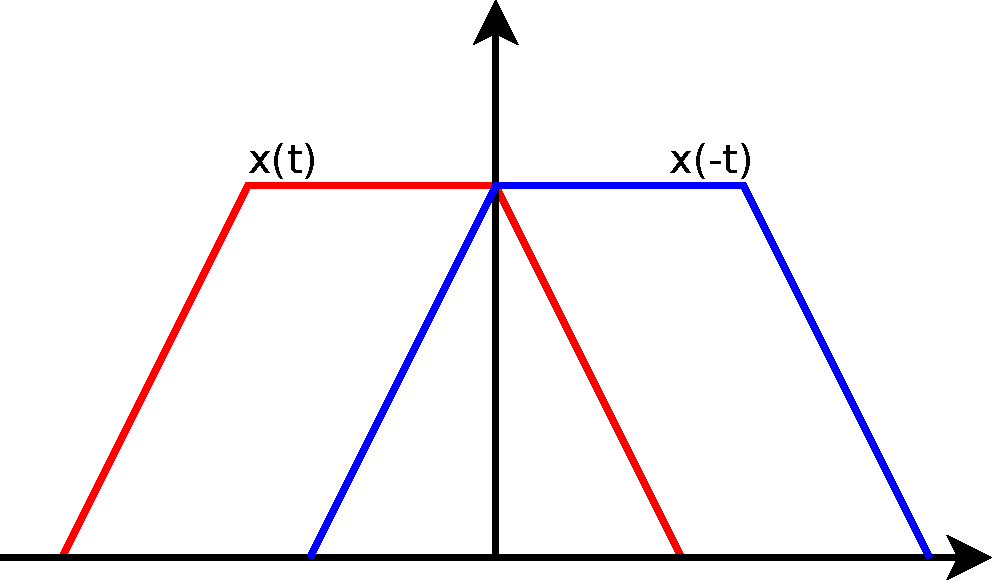
\includegraphics[width=50mm,keepaspectratio=true]{./Elektrotechnik/Bilder/argument.pdf}
  \end{center}
\end{multicols}

\begin{multicols}{2}
\subsubsection*{Nagation des Arguments \texorpdfstring{$t$}{} \\ sowie eine Verschiebung um \texorpdfstring{$t_0$}{}}
\begin{align*}
  &x_{neu}\left(t\right) = x_{alt}\left(t_0 - t\right) \\
  &\text{ mit } t_0 = const.\\
  &x_{neu}\left(t\right) = x_{alt}\left(\tau + 1/2 t_0\right)\\
  &x_{neu}\left(1/2 t_0 - \tau\right) = x_{alt}\left(\tau + 1/2 t_0\right)\\
\end{align*}
\vfill
\begin{center}
 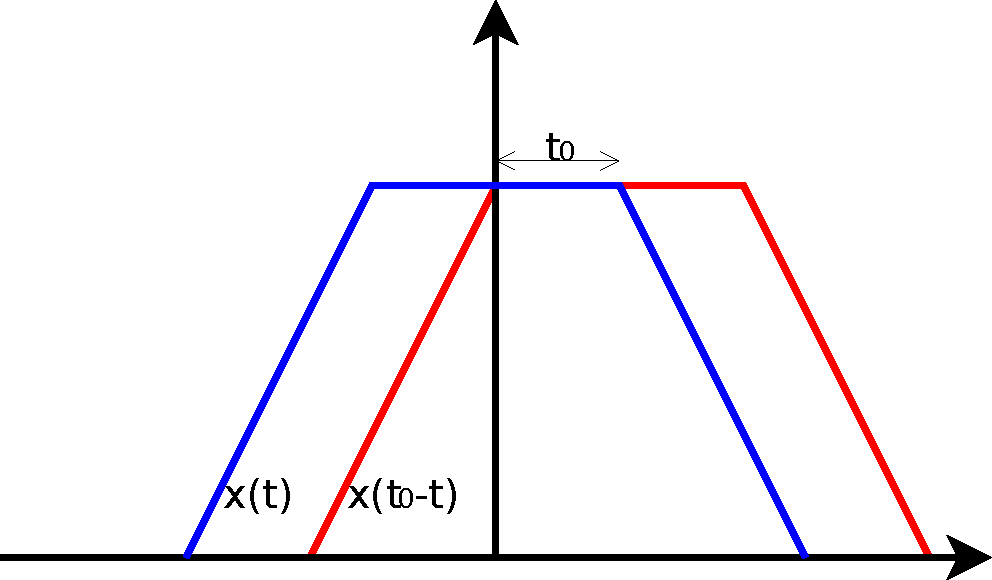
\includegraphics[width=50mm,keepaspectratio=true]{./Elektrotechnik/Bilder/argumentversch.pdf}
\end{center}

\end{multicols}
\begin{itemize}
 \item neue Zeitbasis \(\tau + 1/2 t_0\)
 \item gleiche Funktionswerte, gespiegelt an der Senkrechten von \(1/2 t_0\)
\end{itemize}

\subsubsection*{Skalierungsfaktor \texorpdfstring{$a \neq 0$}{}}
\begin{multicols}{2}
\begin{align*}
  &x_{neu}\left(t\right) = x_{alt}\left(a \cdot t\right) \\
  &\text{ mit } a = const.\\
  &x_{neu}\left(t\right) = x_{alt}\left(\tau\right)\\
  &x_{neu}\left(\tau / a\right) = x_{alt}\left(\tau\right)
\end{align*}
\vfill
\begin{center}
 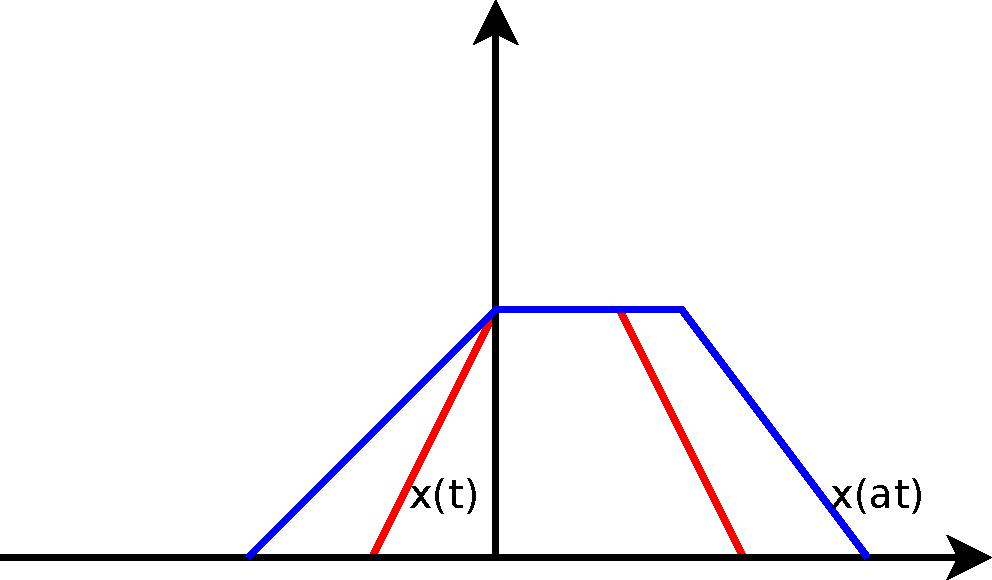
\includegraphics[width=50mm,keepaspectratio=true]{./Elektrotechnik/Bilder/skalierungsfaktor.pdf}
\end{center}

\end{multicols}
\begin{itemize}
 \item neue Zeitbasis \(\tau = a \cdot t\)
 \item gleiche Funktionswerte, wenn die Zeitbasis durch \(a\) geteilt wird
 \item \(a > 1\) Funktion wird gestaucht\\
       \(0 < a < 1\) Funktion wird gestreckt 
\end{itemize}

\subsection*{Einheitssprungfunktion / Deltaimpuls}
\subsubsection*{angenäherte Einheitssprungfunktion
\texorpdfstring{$\tilde{\sigma}\left(t, \epsilon \right)$}{}}
\begin{multicols}{2}
 \begin{itemize}
  \item endlicher Geradenanstieg
  \item Endwert von 1
 \end{itemize}
\vfill
\begin{center}
 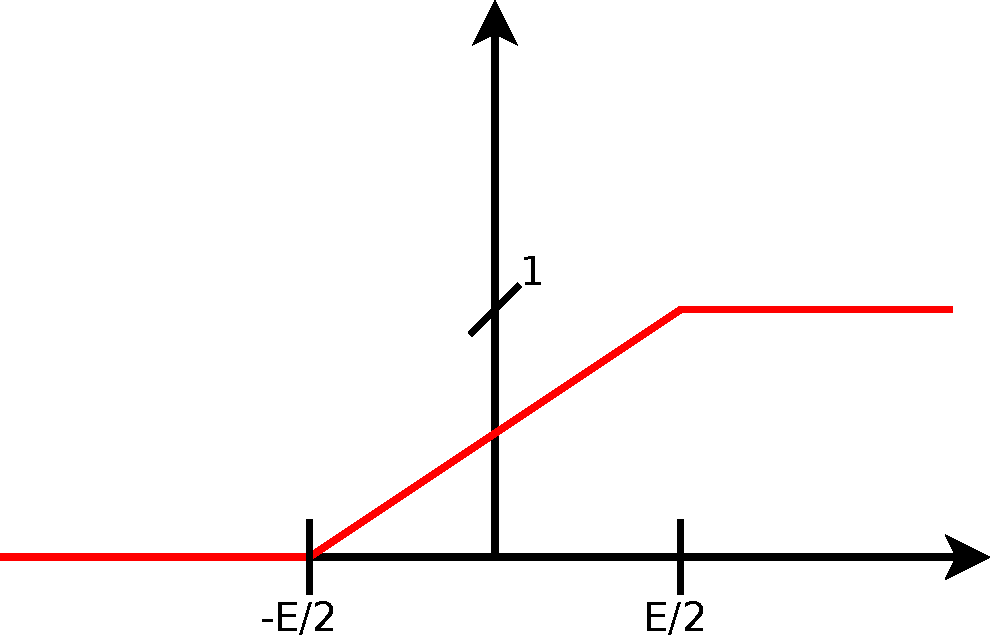
\includegraphics[width=50mm,keepaspectratio=true]{./Elektrotechnik/Bilder/einheitssprungang.pdf}
\end{center}
\vfill
\end{multicols}

\subsubsection*{Einheitsimpuls / Deltaimpuls
\texorpdfstring{$\tilde{\delta}\left(t, \epsilon\right)$}{}}
\begin{multicols}{2}
\begin{itemize}
  \item Fläche des Impulses ist 1
  \item Impulshöhe und Breite variabel
\end{itemize}
\vfill
\begin{center}
	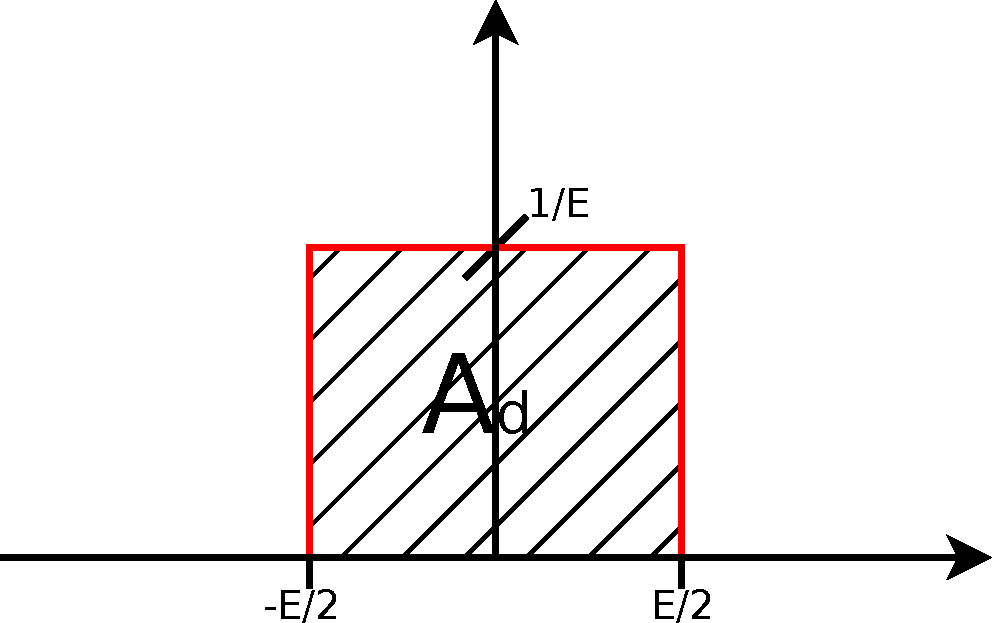
\includegraphics[width=50mm,keepaspectratio=true]{./Elektrotechnik/Bilder/einheitsimpuls.pdf}
\end{center}
\vfill
\end{multicols}


Mathematischer Zusammenhang:
\[
\tilde{\delta} \left(t, \epsilon \right) = \frac{d \tilde{\sigma} \left( t,
\epsilon \right)}{dt} \quad \leftrightarrow \quad \tilde{\sigma} \left( t,
\epsilon \right) = \int_{-\infty}^{t} \tilde{\delta} \left( t, \epsilon \right) dt
\]
Beim Grenzübergang \( \epsilon \rightarrow 0 \) ergibt die
Einheitssprungfunktion \( \sigma \left( t \right) \) bzw. deren Ableitung den
Deltaimpuls \( \delta \left( t \right) \).
\begin{multicols}{2}
\vfill
\[
\delta\left(t\right) = \frac{d \sigma \left(t\right)}{dt} = 
\begin{cases}
+ \infty \text{ für } t = 0 \\
\\
0 \text{ für } t \neq 0
\end{cases}
\]
\vfill
\[
\sigma \left(t\right) = \int_{-\infty}^{t} \delta \left(t\right)dt = 
\begin{cases}
1 \text{ für } t > 0\\
\frac{1}{2} \text{ für } t = 0\\
0 \text{ für } t < 0\\
\end{cases}
\]
\vfill
\end{multicols}

\subsection*{Zusammenhang zwischen Deltaimpuls, Einheitssprungfunktion und Einheitsanstiegsfunktion}

\begin{center}
	% Graphic for TeX using PGF
% Title: /home/Befedo/Documents/eclipse.workspace/Formelsammlung/Elektrotechnik/Bilder/zusammenhang.dia
% Creator: Dia v0.97
% CreationDate: Wed Feb 15 14:26:29 2012
% For: Befedo
% \usepackage{tikz}
% The following commands are not supported in PSTricks at present
% We define them conditionally, so when they are implemented,
% this pgf file will use them.
\ifx\du\undefined
  \newlength{\du}
\fi
\setlength{\du}{15\unitlength}
\begin{tikzpicture}
\pgftransformxscale{1.000000}
\pgftransformyscale{-1.000000}
\definecolor{dialinecolor}{rgb}{0.000000, 0.000000, 0.000000}
\pgfsetstrokecolor{dialinecolor}
\definecolor{dialinecolor}{rgb}{1.000000, 1.000000, 1.000000}
\pgfsetfillcolor{dialinecolor}
\pgfsetlinewidth{0.005000\du}
\pgfsetdash{}{0pt}
\pgfsetdash{}{0pt}
\pgfsetbuttcap
{
\definecolor{dialinecolor}{rgb}{0.000000, 0.000000, 0.000000}
\pgfsetfillcolor{dialinecolor}
% was here!!!
\pgfsetarrowsend{to}
\definecolor{dialinecolor}{rgb}{0.000000, 0.000000, 0.000000}
\pgfsetstrokecolor{dialinecolor}
\draw (1.000000\du,4.000000\du)--(23.000000\du,4.000000\du);
}
\pgfsetlinewidth{0.005000\du}
\pgfsetdash{}{0pt}
\pgfsetdash{}{0pt}
\pgfsetbuttcap
{
\definecolor{dialinecolor}{rgb}{0.000000, 0.000000, 0.000000}
\pgfsetfillcolor{dialinecolor}
% was here!!!
\pgfsetarrowsend{to}
\definecolor{dialinecolor}{rgb}{0.000000, 0.000000, 0.000000}
\pgfsetstrokecolor{dialinecolor}
\draw (5.000000\du,4.000000\du)--(5.000000\du,1.000000\du);
}
\pgfsetlinewidth{0.005000\du}
\pgfsetdash{}{0pt}
\pgfsetdash{}{0pt}
\pgfsetbuttcap
{
\definecolor{dialinecolor}{rgb}{0.000000, 0.000000, 0.000000}
\pgfsetfillcolor{dialinecolor}
% was here!!!
\pgfsetarrowsend{to}
\definecolor{dialinecolor}{rgb}{0.000000, 0.000000, 0.000000}
\pgfsetstrokecolor{dialinecolor}
\draw (12.000000\du,4.000000\du)--(12.000000\du,1.000000\du);
}
\pgfsetlinewidth{0.005000\du}
\pgfsetdash{}{0pt}
\pgfsetdash{}{0pt}
\pgfsetbuttcap
{
\definecolor{dialinecolor}{rgb}{0.000000, 0.000000, 0.000000}
\pgfsetfillcolor{dialinecolor}
% was here!!!
\pgfsetarrowsend{to}
\definecolor{dialinecolor}{rgb}{0.000000, 0.000000, 0.000000}
\pgfsetstrokecolor{dialinecolor}
\draw (19.000000\du,4.000000\du)--(19.000000\du,1.000000\du);
}
\pgfsetlinewidth{0.100000\du}
\pgfsetdash{}{0pt}
\pgfsetdash{}{0pt}
\pgfsetbuttcap
{
\definecolor{dialinecolor}{rgb}{1.000000, 0.000000, 0.000000}
\pgfsetfillcolor{dialinecolor}
% was here!!!
\definecolor{dialinecolor}{rgb}{1.000000, 0.000000, 0.000000}
\pgfsetstrokecolor{dialinecolor}
\draw (3.000000\du,4.000000\du)--(7.000000\du,4.000000\du);
}
\pgfsetlinewidth{0.100000\du}
\pgfsetdash{}{0pt}
\pgfsetdash{}{0pt}
\pgfsetbuttcap
{
\definecolor{dialinecolor}{rgb}{1.000000, 0.000000, 0.000000}
\pgfsetfillcolor{dialinecolor}
% was here!!!
\pgfsetarrowsend{to}
\definecolor{dialinecolor}{rgb}{1.000000, 0.000000, 0.000000}
\pgfsetstrokecolor{dialinecolor}
\draw (5.000000\du,4.000000\du)--(5.000000\du,2.000000\du);
}
\pgfsetlinewidth{0.100000\du}
\pgfsetdash{}{0pt}
\pgfsetdash{}{0pt}
\pgfsetbuttcap
{
\definecolor{dialinecolor}{rgb}{1.000000, 0.000000, 0.000000}
\pgfsetfillcolor{dialinecolor}
% was here!!!
\definecolor{dialinecolor}{rgb}{1.000000, 0.000000, 0.000000}
\pgfsetstrokecolor{dialinecolor}
\draw (12.000000\du,4.000000\du)--(10.000000\du,4.000000\du);
}
\pgfsetlinewidth{0.100000\du}
\pgfsetdash{}{0pt}
\pgfsetdash{}{0pt}
\pgfsetbuttcap
{
\definecolor{dialinecolor}{rgb}{1.000000, 0.000000, 0.000000}
\pgfsetfillcolor{dialinecolor}
% was here!!!
\definecolor{dialinecolor}{rgb}{1.000000, 0.000000, 0.000000}
\pgfsetstrokecolor{dialinecolor}
\draw (14.000000\du,2.000000\du)--(12.000000\du,2.000000\du);
}
\pgfsetlinewidth{0.100000\du}
\pgfsetdash{}{0pt}
\pgfsetdash{}{0pt}
\pgfsetbuttcap
{
\definecolor{dialinecolor}{rgb}{1.000000, 0.000000, 0.000000}
\pgfsetfillcolor{dialinecolor}
% was here!!!
\definecolor{dialinecolor}{rgb}{1.000000, 0.000000, 0.000000}
\pgfsetstrokecolor{dialinecolor}
\draw (17.000000\du,4.000000\du)--(19.000000\du,4.000000\du);
}
\pgfsetlinewidth{0.100000\du}
\pgfsetdash{}{0pt}
\pgfsetdash{}{0pt}
\pgfsetbuttcap
{
\definecolor{dialinecolor}{rgb}{1.000000, 0.000000, 0.000000}
\pgfsetfillcolor{dialinecolor}
% was here!!!
\definecolor{dialinecolor}{rgb}{1.000000, 0.000000, 0.000000}
\pgfsetstrokecolor{dialinecolor}
\draw (19.000000\du,4.000000\du)--(21.000000\du,2.000000\du);
}
\end{tikzpicture}

\end{center}

\begin{align*}
\delta \left( t \right) &= \frac{\mathrm{d} \sigma \left( t \right)}{\mathrm{dt}} =
\frac{\mathrm{d^2} \alpha \left( t \right)}{\mathrm{dt^2}} & \sigma \left( t \right) &=
\int\limits_{-\infty}^{t} \delta \left( t \right) \mathrm{dt} =
\frac{\mathrm{d} \alpha \left( t \right)}{\mathrm{dt}}
\end{align*}

\[
\alpha \left( t \right) = 
\begin{cases}
	t \text{ für } t > 0
	\\
	\\
	0 \text{ für } t \leq 0
\end{cases}
= \int\limits_{-\infty}^{t} \sigma \left( t \right) \mathrm{dt}
= \int\limits_{-\infty}^{t} \int\limits_{-\infty}^{t} \delta \left( t \right) \mathrm{dt}
\]

\subsection*{zeitliche Verschiebung und Wichtung}

\subsubsection*{Deltaimpuls}
	\begin{multicols}{2}
		\vfill
		\begin{align*}
			x \left( t \right) &= A_x \cdot \delta \left( t - t_0 \right) \\
			\left[ x\left(t\right) \right] &= \left[ A_x \right] \cdot \left[ \delta\left( t \right) \right]
		\end{align*}
		\vspace{20mm}
		\vfill
		% Graphic for TeX using PGF
% Title: /home/Befedo/Documents/eclipse.workspace/Formelsammlung/Elektrotechnik/Bilder/delta.dia
% Creator: Dia v0.97
% CreationDate: Wed Feb 15 15:27:30 2012
% For: Befedo
% \usepackage{tikz}
% The following commands are not supported in PSTricks at present
% We define them conditionally, so when they are implemented,
% this pgf file will use them.
\ifx\du\undefined
  \newlength{\du}
\fi
\setlength{\du}{15\unitlength}
\begin{tikzpicture}
\pgftransformxscale{1.000000}
\pgftransformyscale{-1.000000}
\definecolor{dialinecolor}{rgb}{0.000000, 0.000000, 0.000000}
\pgfsetstrokecolor{dialinecolor}
\definecolor{dialinecolor}{rgb}{1.000000, 1.000000, 1.000000}
\pgfsetfillcolor{dialinecolor}
\pgfsetlinewidth{0.100000\du}
\pgfsetdash{}{0pt}
\pgfsetdash{}{0pt}
\pgfsetbuttcap
{
\definecolor{dialinecolor}{rgb}{0.000000, 0.000000, 0.000000}
\pgfsetfillcolor{dialinecolor}
% was here!!!
\definecolor{dialinecolor}{rgb}{0.000000, 0.000000, 0.000000}
\pgfsetstrokecolor{dialinecolor}
\draw (13.500000\du,3.500000\du)--(14.500000\du,2.500000\du);
}
% setfont left to latex
\definecolor{dialinecolor}{rgb}{0.000000, 0.000000, 0.000000}
\pgfsetstrokecolor{dialinecolor}
\node[anchor=west] at (14.500000\du,2.500000\du){};
\pgfsetlinewidth{0.100000\du}
\pgfsetdash{}{0pt}
\pgfsetdash{}{0pt}
\pgfsetbuttcap
{
\definecolor{dialinecolor}{rgb}{0.000000, 0.000000, 0.000000}
\pgfsetfillcolor{dialinecolor}
% was here!!!
\pgfsetarrowsend{stealth}
\definecolor{dialinecolor}{rgb}{0.000000, 0.000000, 0.000000}
\pgfsetstrokecolor{dialinecolor}
\draw (14.000000\du,5.500000\du)--(14.000000\du,1.000000\du);
}
\pgfsetlinewidth{0.100000\du}
\pgfsetdash{}{0pt}
\pgfsetdash{}{0pt}
\pgfsetbuttcap
{
\definecolor{dialinecolor}{rgb}{0.000000, 0.000000, 0.000000}
\pgfsetfillcolor{dialinecolor}
% was here!!!
\pgfsetarrowsend{stealth}
\definecolor{dialinecolor}{rgb}{0.000000, 0.000000, 0.000000}
\pgfsetstrokecolor{dialinecolor}
\draw (9.500000\du,5.500000\du)--(18.500000\du,5.500000\du);
}
\pgfsetlinewidth{0.150000\du}
\pgfsetdash{}{0pt}
\pgfsetdash{}{0pt}
\pgfsetbuttcap
{
\definecolor{dialinecolor}{rgb}{1.000000, 0.000000, 0.000000}
\pgfsetfillcolor{dialinecolor}
% was here!!!
\pgfsetarrowsend{to}
\definecolor{dialinecolor}{rgb}{1.000000, 0.000000, 0.000000}
\pgfsetstrokecolor{dialinecolor}
\draw (16.000000\du,5.500000\du)--(16.000000\du,3.000000\du);
}
% setfont left to latex
\definecolor{dialinecolor}{rgb}{0.000000, 0.000000, 0.000000}
\pgfsetstrokecolor{dialinecolor}
\node[anchor=west] at (14.500000\du,2.500000\du){Ax};
\pgfsetlinewidth{0.100000\du}
\pgfsetdash{}{0pt}
\pgfsetdash{}{0pt}
\pgfsetbuttcap
{
\definecolor{dialinecolor}{rgb}{0.000000, 0.000000, 0.000000}
\pgfsetfillcolor{dialinecolor}
% was here!!!
\definecolor{dialinecolor}{rgb}{0.000000, 0.000000, 0.000000}
\pgfsetstrokecolor{dialinecolor}
\draw (16.000000\du,5.000000\du)--(16.000000\du,6.000000\du);
}
% setfont left to latex
\definecolor{dialinecolor}{rgb}{0.000000, 0.000000, 0.000000}
\pgfsetstrokecolor{dialinecolor}
\node[anchor=west] at (16.200000\du,6.400000\du){t};
% setfont left to latex
\definecolor{dialinecolor}{rgb}{0.000000, 0.000000, 0.000000}
\pgfsetstrokecolor{dialinecolor}
\node[anchor=west] at (16.500000\du,6.500000\du){0};
\end{tikzpicture}

		\vfill
	\end{multicols}
	
\subsubsection*{Einheitssprung}
	\begin{multicols}{2}
		\vfill
		\begin{align*}
			x\left( t \right) &= X_0 \cdot \sigma \left( t - t_0 \right) \\
			\left[ x\left( t \right) \right] &= \left[ X_0 \right]
		\end{align*}
		\vspace{20mm}
		\vfill
		% Graphic for TeX using PGF
% Title: /home/Befedo/Documents/eclipse.workspace/Formelsammlung/Elektrotechnik/Bilder/einheitssprung.dia
% Creator: Dia v0.97
% CreationDate: Wed Feb 15 22:13:28 2012
% For: Befedo
% \usepackage{tikz}
% The following commands are not supported in PSTricks at present
% We define them conditionally, so when they are implemented,
% this pgf file will use them.
\ifx\du\undefined
  \newlength{\du}
\fi
\setlength{\du}{15\unitlength}
\begin{tikzpicture}
\pgftransformxscale{1.000000}
\pgftransformyscale{-1.000000}
\definecolor{dialinecolor}{rgb}{0.000000, 0.000000, 0.000000}
\pgfsetstrokecolor{dialinecolor}
\definecolor{dialinecolor}{rgb}{1.000000, 1.000000, 1.000000}
\pgfsetfillcolor{dialinecolor}
\pgfsetlinewidth{0.100000\du}
\pgfsetdash{}{0pt}
\pgfsetdash{}{0pt}
\pgfsetbuttcap
{
\definecolor{dialinecolor}{rgb}{0.000000, 0.000000, 0.000000}
\pgfsetfillcolor{dialinecolor}
% was here!!!
\definecolor{dialinecolor}{rgb}{0.000000, 0.000000, 0.000000}
\pgfsetstrokecolor{dialinecolor}
\draw (9.000000\du,3.500000\du)--(10.000000\du,2.500000\du);
}
% setfont left to latex
\definecolor{dialinecolor}{rgb}{0.000000, 0.000000, 0.000000}
\pgfsetstrokecolor{dialinecolor}
\node[anchor=west] at (14.500000\du,2.500000\du){};
\pgfsetlinewidth{0.100000\du}
\pgfsetdash{}{0pt}
\pgfsetdash{}{0pt}
\pgfsetbuttcap
{
\definecolor{dialinecolor}{rgb}{0.000000, 0.000000, 0.000000}
\pgfsetfillcolor{dialinecolor}
% was here!!!
\pgfsetarrowsend{stealth}
\definecolor{dialinecolor}{rgb}{0.000000, 0.000000, 0.000000}
\pgfsetstrokecolor{dialinecolor}
\draw (9.500000\du,5.500000\du)--(9.500000\du,1.000000\du);
}
\pgfsetlinewidth{0.100000\du}
\pgfsetdash{}{0pt}
\pgfsetdash{}{0pt}
\pgfsetbuttcap
{
\definecolor{dialinecolor}{rgb}{0.000000, 0.000000, 0.000000}
\pgfsetfillcolor{dialinecolor}
% was here!!!
\pgfsetarrowsend{stealth}
\definecolor{dialinecolor}{rgb}{0.000000, 0.000000, 0.000000}
\pgfsetstrokecolor{dialinecolor}
\draw (9.500000\du,5.500000\du)--(18.500000\du,5.500000\du);
}
% setfont left to latex
\definecolor{dialinecolor}{rgb}{0.000000, 0.000000, 0.000000}
\pgfsetstrokecolor{dialinecolor}
\node[anchor=west] at (10.000000\du,2.500000\du){X};
\pgfsetlinewidth{0.100000\du}
\pgfsetdash{}{0pt}
\pgfsetdash{}{0pt}
\pgfsetbuttcap
{
\definecolor{dialinecolor}{rgb}{0.000000, 0.000000, 0.000000}
\pgfsetfillcolor{dialinecolor}
% was here!!!
\definecolor{dialinecolor}{rgb}{0.000000, 0.000000, 0.000000}
\pgfsetstrokecolor{dialinecolor}
\draw (14.000000\du,5.000000\du)--(14.000000\du,6.000000\du);
}
% setfont left to latex
\definecolor{dialinecolor}{rgb}{0.000000, 0.000000, 0.000000}
\pgfsetstrokecolor{dialinecolor}
\node[anchor=west] at (14.000000\du,6.500000\du){t};
% setfont left to latex
\definecolor{dialinecolor}{rgb}{0.000000, 0.000000, 0.000000}
\pgfsetstrokecolor{dialinecolor}
\node[anchor=west] at (14.300000\du,6.600000\du){0};
\pgfsetlinewidth{0.150000\du}
\pgfsetdash{}{0pt}
\pgfsetdash{}{0pt}
\pgfsetbuttcap
{
\definecolor{dialinecolor}{rgb}{1.000000, 0.000000, 0.000000}
\pgfsetfillcolor{dialinecolor}
% was here!!!
\definecolor{dialinecolor}{rgb}{1.000000, 0.000000, 0.000000}
\pgfsetstrokecolor{dialinecolor}
\draw (9.500000\du,5.500000\du)--(14.000000\du,5.500000\du);
}
\pgfsetlinewidth{0.150000\du}
\pgfsetdash{}{0pt}
\pgfsetdash{}{0pt}
\pgfsetbuttcap
{
\definecolor{dialinecolor}{rgb}{1.000000, 0.000000, 0.000000}
\pgfsetfillcolor{dialinecolor}
% was here!!!
\definecolor{dialinecolor}{rgb}{1.000000, 0.000000, 0.000000}
\pgfsetstrokecolor{dialinecolor}
\draw (14.000000\du,3.000000\du)--(17.500000\du,3.000000\du);
}
% setfont left to latex
\definecolor{dialinecolor}{rgb}{0.000000, 0.000000, 0.000000}
\pgfsetstrokecolor{dialinecolor}
\node[anchor=west] at (10.435781\du,2.493530\du){0};
\end{tikzpicture}

		\vfill
	\end{multicols}
	
\subsubsection*{Einheitsanstiegsfunktion}
	\begin{multicols}{2}
		\vfill
		\begin{align*}
			x \left( t \right) &= m \cdot \alpha \left( t - t_0 \right) \\
			\left[ x \left( t \right) \right] &= \left[ m \right] \cdot \left[ \alpha \left(t\right) \right]
		\end{align*}
		\vspace{20mm}
		\vfill
		% Graphic for TeX using PGF
% Title: /home/Befedo/Documents/eclipse.workspace/Formelsammlung/Elektrotechnik/Bilder/einheitsanstieg.dia
% Creator: Dia v0.97
% CreationDate: Wed Feb 15 16:40:58 2012
% For: Befedo
% \usepackage{tikz}
% The following commands are not supported in PSTricks at present
% We define them conditionally, so when they are implemented,
% this pgf file will use them.
\ifx\du\undefined
  \newlength{\du}
\fi
\setlength{\du}{15\unitlength}
\begin{tikzpicture}
\pgftransformxscale{1.000000}
\pgftransformyscale{-1.000000}
\definecolor{dialinecolor}{rgb}{0.000000, 0.000000, 0.000000}
\pgfsetstrokecolor{dialinecolor}
\definecolor{dialinecolor}{rgb}{1.000000, 1.000000, 1.000000}
\pgfsetfillcolor{dialinecolor}
% setfont left to latex
\definecolor{dialinecolor}{rgb}{0.000000, 0.000000, 0.000000}
\pgfsetstrokecolor{dialinecolor}
\node[anchor=west] at (14.500000\du,2.500000\du){};
\pgfsetlinewidth{0.100000\du}
\pgfsetdash{}{0pt}
\pgfsetdash{}{0pt}
\pgfsetbuttcap
{
\definecolor{dialinecolor}{rgb}{0.000000, 0.000000, 0.000000}
\pgfsetfillcolor{dialinecolor}
% was here!!!
\pgfsetarrowsend{stealth}
\definecolor{dialinecolor}{rgb}{0.000000, 0.000000, 0.000000}
\pgfsetstrokecolor{dialinecolor}
\draw (9.500000\du,5.500000\du)--(9.500000\du,1.000000\du);
}
\pgfsetlinewidth{0.100000\du}
\pgfsetdash{}{0pt}
\pgfsetdash{}{0pt}
\pgfsetbuttcap
{
\definecolor{dialinecolor}{rgb}{0.000000, 0.000000, 0.000000}
\pgfsetfillcolor{dialinecolor}
% was here!!!
\pgfsetarrowsend{stealth}
\definecolor{dialinecolor}{rgb}{0.000000, 0.000000, 0.000000}
\pgfsetstrokecolor{dialinecolor}
\draw (9.500000\du,5.500000\du)--(18.500000\du,5.500000\du);
}
\pgfsetlinewidth{0.100000\du}
\pgfsetdash{}{0pt}
\pgfsetdash{}{0pt}
\pgfsetbuttcap
{
\definecolor{dialinecolor}{rgb}{0.000000, 0.000000, 0.000000}
\pgfsetfillcolor{dialinecolor}
% was here!!!
\definecolor{dialinecolor}{rgb}{0.000000, 0.000000, 0.000000}
\pgfsetstrokecolor{dialinecolor}
\draw (14.000000\du,5.000000\du)--(14.000000\du,6.000000\du);
}
% setfont left to latex
\definecolor{dialinecolor}{rgb}{0.000000, 0.000000, 0.000000}
\pgfsetstrokecolor{dialinecolor}
\node[anchor=west] at (14.000000\du,6.500000\du){t};
% setfont left to latex
\definecolor{dialinecolor}{rgb}{0.000000, 0.000000, 0.000000}
\pgfsetstrokecolor{dialinecolor}
\node[anchor=west] at (14.300000\du,6.600000\du){0};
\pgfsetlinewidth{0.150000\du}
\pgfsetdash{}{0pt}
\pgfsetdash{}{0pt}
\pgfsetbuttcap
{
\definecolor{dialinecolor}{rgb}{1.000000, 0.000000, 0.000000}
\pgfsetfillcolor{dialinecolor}
% was here!!!
\definecolor{dialinecolor}{rgb}{1.000000, 0.000000, 0.000000}
\pgfsetstrokecolor{dialinecolor}
\draw (9.500000\du,5.500000\du)--(14.000000\du,5.500000\du);
}
\pgfsetlinewidth{0.150000\du}
\pgfsetdash{}{0pt}
\pgfsetdash{}{0pt}
\pgfsetbuttcap
{
\definecolor{dialinecolor}{rgb}{1.000000, 0.000000, 0.000000}
\pgfsetfillcolor{dialinecolor}
% was here!!!
\definecolor{dialinecolor}{rgb}{1.000000, 0.000000, 0.000000}
\pgfsetstrokecolor{dialinecolor}
\draw (14.000000\du,5.500000\du)--(17.500000\du,2.500000\du);
}
\end{tikzpicture}

		\vfill
	\end{multicols}
	
\newpage
\section{Signale}
\textbf{Definition:}
Ein Signal ist eine zeitlich und / oder örtlich veränderliche Größe (physikalisch).
Die Veränderung dieser physikalischen Größe, sagt nichts über Ihren Informationsgehalt aus.
	
\begin{center}
	% Graphic for TeX using PGF
% Title: /home/Befedo/Documents/eclipse.workspace/Formelsammlung/Elektrotechnik/Bilder/signalstatistik.dia
% Creator: Dia v0.97
% CreationDate: Wed Feb 15 23:22:16 2012
% For: Befedo
% \usepackage{tikz}
% The following commands are not supported in PSTricks at present
% We define them conditionally, so when they are implemented,
% this pgf file will use them.
\ifx\du\undefined
  \newlength{\du}
\fi
\setlength{\du}{15\unitlength}
\begin{tikzpicture}
\pgftransformxscale{1.000000}
\pgftransformyscale{-1.000000}
\definecolor{dialinecolor}{rgb}{0.000000, 0.000000, 0.000000}
\pgfsetstrokecolor{dialinecolor}
\definecolor{dialinecolor}{rgb}{1.000000, 1.000000, 1.000000}
\pgfsetfillcolor{dialinecolor}
\pgfsetlinewidth{0.100000\du}
\pgfsetdash{}{0pt}
{\pgfsetcornersarced{\pgfpoint{0.500000\du}{0.500000\du}}\definecolor{dialinecolor}{rgb}{1.000000, 1.000000, 1.000000}
\pgfsetfillcolor{dialinecolor}
\fill (9.500000\du,0.500000\du)--(9.500000\du,2.300000\du)--(13.500000\du,2.300000\du)--(13.500000\du,0.500000\du)--cycle;
}{\pgfsetcornersarced{\pgfpoint{0.500000\du}{0.500000\du}}\definecolor{dialinecolor}{rgb}{0.000000, 0.000000, 0.000000}
\pgfsetstrokecolor{dialinecolor}
\draw (9.500000\du,0.500000\du)--(9.500000\du,2.300000\du)--(13.500000\du,2.300000\du)--(13.500000\du,0.500000\du)--cycle;
}% setfont left to latex
\definecolor{dialinecolor}{rgb}{0.000000, 0.000000, 0.000000}
\pgfsetstrokecolor{dialinecolor}
\node at (11.500000\du,1.595000\du){Signal};
\pgfsetlinewidth{0.100000\du}
\pgfsetdash{}{0pt}
{\pgfsetcornersarced{\pgfpoint{0.500000\du}{0.500000\du}}\definecolor{dialinecolor}{rgb}{1.000000, 1.000000, 1.000000}
\pgfsetfillcolor{dialinecolor}
\fill (2.500000\du,3.500000\du)--(2.500000\du,5.300000\du)--(7.830000\du,5.300000\du)--(7.830000\du,3.500000\du)--cycle;
}{\pgfsetcornersarced{\pgfpoint{0.500000\du}{0.500000\du}}\definecolor{dialinecolor}{rgb}{0.000000, 0.000000, 0.000000}
\pgfsetstrokecolor{dialinecolor}
\draw (2.500000\du,3.500000\du)--(2.500000\du,5.300000\du)--(7.830000\du,5.300000\du)--(7.830000\du,3.500000\du)--cycle;
}% setfont left to latex
\definecolor{dialinecolor}{rgb}{0.000000, 0.000000, 0.000000}
\pgfsetstrokecolor{dialinecolor}
\node at (5.165000\du,4.595000\du){Energiesignal};
\pgfsetlinewidth{0.100000\du}
\pgfsetdash{}{0pt}
{\pgfsetcornersarced{\pgfpoint{0.500000\du}{0.500000\du}}\definecolor{dialinecolor}{rgb}{1.000000, 1.000000, 1.000000}
\pgfsetfillcolor{dialinecolor}
\fill (15.000000\du,3.500000\du)--(15.000000\du,5.300000\du)--(20.612500\du,5.300000\du)--(20.612500\du,3.500000\du)--cycle;
}{\pgfsetcornersarced{\pgfpoint{0.500000\du}{0.500000\du}}\definecolor{dialinecolor}{rgb}{0.000000, 0.000000, 0.000000}
\pgfsetstrokecolor{dialinecolor}
\draw (15.000000\du,3.500000\du)--(15.000000\du,5.300000\du)--(20.612500\du,5.300000\du)--(20.612500\du,3.500000\du)--cycle;
}% setfont left to latex
\definecolor{dialinecolor}{rgb}{0.000000, 0.000000, 0.000000}
\pgfsetstrokecolor{dialinecolor}
\node at (17.806250\du,4.595000\du){Leistungsignal};
\pgfsetlinewidth{0.100000\du}
\pgfsetdash{}{0pt}
\pgfsetdash{}{0pt}
\pgfsetbuttcap
{
\definecolor{dialinecolor}{rgb}{0.000000, 0.000000, 0.000000}
\pgfsetfillcolor{dialinecolor}
% was here!!!
\pgfsetarrowsend{stealth}
\definecolor{dialinecolor}{rgb}{0.000000, 0.000000, 0.000000}
\pgfsetstrokecolor{dialinecolor}
\draw (9.500000\du,2.300000\du)--(8.000000\du,3.500000\du);
}
\pgfsetlinewidth{0.100000\du}
\pgfsetdash{}{0pt}
\pgfsetdash{}{0pt}
\pgfsetbuttcap
{
\definecolor{dialinecolor}{rgb}{0.000000, 0.000000, 0.000000}
\pgfsetfillcolor{dialinecolor}
% was here!!!
\pgfsetarrowsend{stealth}
\definecolor{dialinecolor}{rgb}{0.000000, 0.000000, 0.000000}
\pgfsetstrokecolor{dialinecolor}
\draw (13.500000\du,2.300000\du)--(15.000000\du,3.500000\du);
}
\pgfsetlinewidth{0.100000\du}
\pgfsetdash{}{0pt}
\pgfsetdash{}{0pt}
\pgfsetbuttcap
{
\definecolor{dialinecolor}{rgb}{0.000000, 0.000000, 0.000000}
\pgfsetfillcolor{dialinecolor}
% was here!!!
\pgfsetarrowsend{stealth}
\definecolor{dialinecolor}{rgb}{0.000000, 0.000000, 0.000000}
\pgfsetstrokecolor{dialinecolor}
\draw (2.500000\du,5.300000\du)--(1.500000\du,7.000000\du);
}
\pgfsetlinewidth{0.100000\du}
\pgfsetdash{}{0pt}
\pgfsetdash{}{0pt}
\pgfsetbuttcap
{
\definecolor{dialinecolor}{rgb}{0.000000, 0.000000, 0.000000}
\pgfsetfillcolor{dialinecolor}
% was here!!!
\pgfsetarrowsend{stealth}
\definecolor{dialinecolor}{rgb}{0.000000, 0.000000, 0.000000}
\pgfsetstrokecolor{dialinecolor}
\draw (5.165000\du,5.300000\du)--(5.500000\du,6.975000\du);
}
\pgfsetlinewidth{0.100000\du}
\pgfsetdash{}{0pt}
\pgfsetdash{}{0pt}
\pgfsetbuttcap
{
\definecolor{dialinecolor}{rgb}{0.000000, 0.000000, 0.000000}
\pgfsetfillcolor{dialinecolor}
% was here!!!
\pgfsetarrowsend{stealth}
\definecolor{dialinecolor}{rgb}{0.000000, 0.000000, 0.000000}
\pgfsetstrokecolor{dialinecolor}
\draw (7.830000\du,5.300000\du)--(10.000000\du,7.000000\du);
}
\pgfsetlinewidth{0.100000\du}
\pgfsetdash{}{0pt}
\pgfsetdash{}{0pt}
\pgfsetbuttcap
{
\definecolor{dialinecolor}{rgb}{0.000000, 0.000000, 0.000000}
\pgfsetfillcolor{dialinecolor}
% was here!!!
\pgfsetarrowsend{stealth}
\definecolor{dialinecolor}{rgb}{0.000000, 0.000000, 0.000000}
\pgfsetstrokecolor{dialinecolor}
\draw (17.806250\du,5.300000\du)--(18.000000\du,7.000000\du);
}
\pgfsetlinewidth{0.100000\du}
\pgfsetdash{}{0pt}
\pgfsetdash{}{0pt}
\pgfsetmiterjoin
\definecolor{dialinecolor}{rgb}{1.000000, 1.000000, 1.000000}
\pgfsetfillcolor{dialinecolor}
\fill (0.000000\du,7.000000\du)--(0.000000\du,8.500000\du)--(3.000000\du,8.500000\du)--(3.000000\du,7.000000\du)--cycle;
\definecolor{dialinecolor}{rgb}{0.000000, 0.000000, 0.000000}
\pgfsetstrokecolor{dialinecolor}
\draw (0.000000\du,7.000000\du)--(0.000000\du,8.500000\du)--(3.000000\du,8.500000\du)--(3.000000\du,7.000000\du)--cycle;
% setfont left to latex
\definecolor{dialinecolor}{rgb}{0.000000, 0.000000, 0.000000}
\pgfsetstrokecolor{dialinecolor}
\node at (1.500000\du,7.500000\du){zeitlich};
% setfont left to latex
\definecolor{dialinecolor}{rgb}{0.000000, 0.000000, 0.000000}
\pgfsetstrokecolor{dialinecolor}
\node at (1.500000\du,8.088433\du){begrenzt};
\pgfsetlinewidth{0.100000\du}
\pgfsetdash{}{0pt}
\pgfsetdash{}{0pt}
\pgfsetmiterjoin
\definecolor{dialinecolor}{rgb}{1.000000, 1.000000, 1.000000}
\pgfsetfillcolor{dialinecolor}
\fill (3.500000\du,6.975000\du)--(3.500000\du,8.475000\du)--(7.500000\du,8.475000\du)--(7.500000\du,6.975000\du)--cycle;
\definecolor{dialinecolor}{rgb}{0.000000, 0.000000, 0.000000}
\pgfsetstrokecolor{dialinecolor}
\draw (3.500000\du,6.975000\du)--(3.500000\du,8.475000\du)--(7.500000\du,8.475000\du)--(7.500000\du,6.975000\du)--cycle;
% setfont left to latex
\definecolor{dialinecolor}{rgb}{0.000000, 0.000000, 0.000000}
\pgfsetstrokecolor{dialinecolor}
\node at (5.500000\du,7.500000\du){abklingende};
% setfont left to latex
\definecolor{dialinecolor}{rgb}{0.000000, 0.000000, 0.000000}
\pgfsetstrokecolor{dialinecolor}
\node at (5.500000\du,8.088433\du){Amplitude};
\pgfsetlinewidth{0.100000\du}
\pgfsetdash{}{0pt}
\pgfsetdash{}{0pt}
\pgfsetmiterjoin
\definecolor{dialinecolor}{rgb}{1.000000, 1.000000, 1.000000}
\pgfsetfillcolor{dialinecolor}
\fill (8.000000\du,7.000000\du)--(8.000000\du,8.500000\du)--(12.000000\du,8.500000\du)--(12.000000\du,7.000000\du)--cycle;
\definecolor{dialinecolor}{rgb}{0.000000, 0.000000, 0.000000}
\pgfsetstrokecolor{dialinecolor}
\draw (8.000000\du,7.000000\du)--(8.000000\du,8.500000\du)--(12.000000\du,8.500000\du)--(12.000000\du,7.000000\du)--cycle;
% setfont left to latex
\definecolor{dialinecolor}{rgb}{0.000000, 0.000000, 0.000000}
\pgfsetstrokecolor{dialinecolor}
\node at (10.000000\du,7.500000\du){sehr große};
% setfont left to latex
\definecolor{dialinecolor}{rgb}{0.000000, 0.000000, 0.000000}
\pgfsetstrokecolor{dialinecolor}
\node at (10.000000\du,8.088433\du){Pausenzeit};
\pgfsetlinewidth{0.100000\du}
\pgfsetdash{}{0pt}
\pgfsetdash{}{0pt}
\pgfsetmiterjoin
\definecolor{dialinecolor}{rgb}{1.000000, 1.000000, 1.000000}
\pgfsetfillcolor{dialinecolor}
\fill (16.000000\du,7.000000\du)--(16.000000\du,8.500000\du)--(20.000000\du,8.500000\du)--(20.000000\du,7.000000\du)--cycle;
\definecolor{dialinecolor}{rgb}{0.000000, 0.000000, 0.000000}
\pgfsetstrokecolor{dialinecolor}
\draw (16.000000\du,7.000000\du)--(16.000000\du,8.500000\du)--(20.000000\du,8.500000\du)--(20.000000\du,7.000000\du)--cycle;
% setfont left to latex
\definecolor{dialinecolor}{rgb}{0.000000, 0.000000, 0.000000}
\pgfsetstrokecolor{dialinecolor}
\node at (18.000000\du,7.500000\du){zeitlich};
% setfont left to latex
\definecolor{dialinecolor}{rgb}{0.000000, 0.000000, 0.000000}
\pgfsetstrokecolor{dialinecolor}
\node at (18.000000\du,8.088433\du){unbegrenzt};
% setfont left to latex
\definecolor{dialinecolor}{rgb}{0.000000, 0.000000, 0.000000}
\pgfsetstrokecolor{dialinecolor}
\node[anchor=west] at (0.500000\du,9.000000\du){-rect};
% setfont left to latex
\definecolor{dialinecolor}{rgb}{0.000000, 0.000000, 0.000000}
\pgfsetstrokecolor{dialinecolor}
\node[anchor=west] at (0.500000\du,9.447322\du){};
% setfont left to latex
\definecolor{dialinecolor}{rgb}{0.000000, 0.000000, 0.000000}
\pgfsetstrokecolor{dialinecolor}
\node[anchor=west] at (0.500000\du,9.894644\du){-Delta};
% setfont left to latex
\definecolor{dialinecolor}{rgb}{0.000000, 0.000000, 0.000000}
\pgfsetstrokecolor{dialinecolor}
\node[anchor=west] at (4.000000\du,9.000000\du){-exp-F.};
% setfont left to latex
\definecolor{dialinecolor}{rgb}{0.000000, 0.000000, 0.000000}
\pgfsetstrokecolor{dialinecolor}
\node[anchor=west] at (8.500000\du,9.000000\du){-Burst};
% setfont left to latex
\definecolor{dialinecolor}{rgb}{0.000000, 0.000000, 0.000000}
\pgfsetstrokecolor{dialinecolor}
\node[anchor=west] at (8.500000\du,9.447322\du){};
% setfont left to latex
\definecolor{dialinecolor}{rgb}{0.000000, 0.000000, 0.000000}
\pgfsetstrokecolor{dialinecolor}
\node[anchor=west] at (8.500000\du,9.894644\du){-Ethernet Paket};
% setfont left to latex
\definecolor{dialinecolor}{rgb}{0.000000, 0.000000, 0.000000}
\pgfsetstrokecolor{dialinecolor}
\node[anchor=west] at (16.500000\du,9.000000\du){-Sinus};
% setfont left to latex
\definecolor{dialinecolor}{rgb}{0.000000, 0.000000, 0.000000}
\pgfsetstrokecolor{dialinecolor}
\node[anchor=west] at (16.500000\du,9.447322\du){};
% setfont left to latex
\definecolor{dialinecolor}{rgb}{0.000000, 0.000000, 0.000000}
\pgfsetstrokecolor{dialinecolor}
\node[anchor=west] at (16.500000\du,9.894644\du){-Rauschen};
\end{tikzpicture}

\end{center}

\subsection*{Energiewandlung}
\begin{align*}
	E_R &= \int\limits_{-\infty}^{\infty} u \left( t \right) \cdot i \left( t \right) \mathrm{dt} &
	\left[ E_R \right] &= V \cdot A \cdot s = Ws 
	\\
	\text{mit } i \left( t \right) &= \frac{u \left( t \right)}{R} \text{ folgt}
	\\
	E_R &= \frac{1}{R}\int\limits_{-\infty}^{\infty}u^2 \left( t \right) \mathrm{dt}  
\end{align*}

\subsection*{Momentanleistung \texorpdfstring{$P_r\left(t_1\right)$}}
\begin{align*}
	P_R \left(t_1\right) &= u\left(t_1\right) \cdot i\left(t_1\right) &
	&\left[P_R\left(t_1\right)\right] = W
	\\
	P_R &= U_0 \cdot I_0 = \frac{U_0^2}{R} & &\text{ bei Gleichleistung}	
\end{align*}

\subsection*{Mittlere Leistung \texorpdfstring{$P_R$}}
\begin{align*}
	P_R &= \lim\limits_{T \to \infty} \frac{1}{T} \int\limits_{t_1}^{t_1 + T} u\left(t\right) \cdot
	i\left(t\right) \mathrm{dt} & \left[P_R\right] &= W
	\\
	    &= \frac{1}{R} \cdot \lim\limits_{T \to \infty} \frac{1}{T} \int\limits_{t_1}^{t_1 + T} u^2
		\left(t\right) \mathrm{dt}
	\\
	&\textbf{Spezialfall: } \text{Periodische Signalverläufe}
	\\
		&= \frac{1}{n \cdot t_P} \int\limits_{t_1}^{t_1 + n\cdot t_P} u_P \left(t\right) \cdot
		i_P\left(t\right) \mathrm{dt} = \frac{1}{R \cdot n \cdot t_P} \int\limits_{t_1}^{t_1 + n \cdot
		t_P} u_P^2 \left(t\right) \mathrm{dt}
\end{align*}
\[T \text{: Betrachtungszeit, Meßdauer } t_1 \text{: Startzeitpunkt } t_P \text{: Periodendauer } R
= const.\]

\subsection*{Signalenergie / Impulsenergie / Impulsmoment 2. Ordnung \texorpdfstring{$E_U$}}

Nur für Energiesignale sinnvoll.
\begin{align*}
	E_U &= {m_i}_2 = \int\limits_{-\infty}^{\infty}u^2\left(t\right) \mathrm{dt} & \left[E_U\right] =
	{V^2}s
\end{align*}

Zeitdiskrete Signalverläufe:
\begin{align*}
	E_X &= {m_i}_2 = \sum\limits_{k = -\infty}^{\infty} X^2_q\left(k\right) &	\left[E_X\right] &= 1
\end{align*}

Entnormierung über einem realen Widerstand:
\begin{align*}
	E_R &= E_U \cdot \frac{1}{R} & \left[E_R\right] &= Ws
\end{align*}

\subsection*{Signalleistung \texorpdfstring{$P_u$} // Gesamtsignalleistung \texorpdfstring{$P_i$} //
quadratischer Mittelwert \texorpdfstring{$\overline{u^2}$} // gewöhnliches Moment 2. Ordnung
\texorpdfstring{$m_2$} }

Nur für Leistungssignale sinnvoll.
\begin{align*}
	P_u &= \overline{u^2} = m_2 = \lim\limits_{T \to \infty} \frac{1}{T} \int\limits_{t_1}^{t_1 +
	T}u^2\left(t\right) \mathrm{dt} & \left[P_u\right] &= V^2
\end{align*}

\begin{align*}
	&\textbf{Spezialfall: } \text{Periodische Signalverläufe}
	\\
	P_u &= \overline{u^2} = m_2 = \frac{1}{t_p} \int\limits_{t_1}^{t_1 + t_p}u^2_p\left(t\right)
	\mathrm{dt}
	\\
&\textbf{Spezialfall: } \text{zeitdiskrete Signalverläufe}
	\\
	&\text{beliebiges nichtperiodisches Signal:} & &\text{periodisches Signal:}
	\\
	P_X &= \lim\limits_{N \to \infty} \frac{1}{N} \cdot \sum\limits_{k = k_1}^{k_1 +
	N - 1} X_q^2\left(k\right) &
	P_X &= \frac{1}{N_P} \sum\limits_{k = k_1}^{k_1 + N - 1}X_q^2\left(k\right)_P
	\\
&\textbf{Spezialfall: } \text{konstannte Werte}
	\\
	P_X &= X^2_q\left(k_1\right)_k
\end{align*}

Entnormierung über einem realen Widerstand:
\begin{align*}
	P_R &= P_U \cdot \frac{1}{R} & \left[P_R\right] &= W
\end{align*}

\subsection*{Signalenergie\texorpdfstring{$\leftrightarrow$}/Signalleistung}
\begin{tabularx}{\textwidth}{|X|X|X|}\hline
					& Energiesignal 	& Leistungssignal	\\ \hline
	Signalenergie	& endlicher Wert	& \(+\infty\)		\\ \hline
	Signalleistung	& \(0\)				& endlicher Wert	\\ \hline
\end{tabularx}

\section{Signalbeschreibung Leistungssignale}
\subsection*{Effektivwert}
Energiesignale haben einen Effektivwert von Null.
\[
u_{eff} = \sqrt{P_u} = \sqrt{\lim\limits_{T \to \infty} \frac{1}{T} \int\limits_{t_1}^{t_1 +
	T}u^2\left(t\right) \mathrm{dt}}
\]
\textbf{Spezialfall: } \text{zeitdiskrete Signalverläufe}
\[
X_{eff} = \sqrt{P_X} = \sqrt{\lim\limits_{N \to \infty} \frac{1}{N} \cdot \sum\limits_{k = k_1}^{k_1 +
	N - 1} X_q^2\left(k\right)}
\]

\subsection*{Gleichanteil / linearer Mittelwert / gewöhnliches Moment 1. Ordnung
\texorpdfstring{$m_1$}} 
Enrgiesignale haben einen Gleichanteil von Null.

\begin{align*}
&\textbf{beliebige Signalverläufe}
	\\
	\overline{x} &= m_1 = \lim\limits_{T \to \infty} \frac{1}{T} \int\limits_{t_1}^{t_1 + T}
	x\left(t\right) \mathrm{dt} & \left[\overline{x}\right] = \left[x\right]
	\\
&\textbf{periodische Signalverläufe}
	\\
	\overline{x} &= m_1 = \frac{1}{t_p} \int\limits_{t_1}^{t_1 + t_p}
	x\left(t\right) \mathrm{dt} & \left[\overline{x}\right] = \left[x\right]
	\\
&\textbf{zeitdiskrete Signalverläufe}
	\\
	\overline{x_k} &= \lim\limits_{N \to \infty} \frac{1}{N} \sum\limits_{k = k_1}^{k_1 + N -
	1}x_q\left(k\right)
	\\
&\textbf{periodische zeitdiskrete Signalverläufe}
	\\
	\overline{x_k} &= \frac{1}{N_p} \sum\limits_{k = k_1}^{k_1 + N -
	1}x_q\left(k\right)_p
\end{align*}

\subsection*{Signalgleichleistung / quadrierter linearer Mittelwert
\texorpdfstring{$\overline{u}^2$} // quadriertes gewöhnliches Moment 1. Ordnung
\texorpdfstring{$m_1^2$}}
Energiesignale haben eine Signalgleichleistung von Null.

\begin{align*}
&\textbf{beliebige Signalverläufe}
	\\
	P_{u_{=}} &= \left[\overline{u}\right]^2 = m_1^2 = \left[ \lim\limits_{T \to \infty} \frac{1}{T} \int\limits_{t_1}^{t_1 + T}
	u\left(t\right) \mathrm{dt} \right]^2 & \left[ P_{u_{=}} \right] &= V^2
	\\
&\textbf{zeitdiskrete Signalverläufe}
	\\
	P_{X_{=}} &= \left[\overline{x}\right]^2 = m_1^2 = \left[ \lim\limits_{N \to \infty} \frac{1}{N}
	\sum\limits_{k = k_1}^{k_1 + N - 1}X_q\left(k\right) \right]^2 & \left[ P_{X_{=}} \right] &= 1
	\\
&\textbf{Entnormierung}
	\\
	P_{R_{=}} &= \frac{P_{u_{=}}}{R} & \left[ P_{R_{=}} \right] &= W
\end{align*}

\subsection*{Signalwechselleistung \texorpdfstring{$P_{u_{\sim}}$} // Varianz
\texorpdfstring{$\sigma^2$} // zentrales Moment 2. Ordnung \texorpdfstring{$\mu_2$}}
Energiesignale haben eine Signalwechselleistung von Null.
\begin{align*}
	P_{u_{\sim}} &= \sigma^2 = \mu_2 = \lim\limits_{T \to \infty} \frac{1}{T} \int\limits_{t_1}^{t_1 +
	T} \left[ u\left(t\right) - \overline{u} \right]^2 \mathrm{dt}
	\\
	&\textbf{periodischer Spannungsverlauf}
	\\
	P_{p_{\sim}} &= \frac{1}{t_p} \int\limits_{t_1}^{t_1 + t_p} \left[ u\left(t\right) - \overline{u}
	\right]^2 \mathrm{dt}
	\\
	&\textbf{zeitdiskrete Signale}
	\\
	P_{X_{\sim}} &= \lim\limits_{N \to \infty} \frac{1}{N} \sum\limits_{k = k_1}^{k_1 + N -1}\left[
 	X_q \left(k\right) - \overline{X} \right]^2
	\\
	&\textbf{periodische zeitdiskrete Signale}
	\\
	P_{X_{\sim}} &= \frac{1}{N_p} \sum\limits_{k = k_1}^{k_1 + N -1}\left[
 	X_q \left(k\right)_p - \overline{X} \right]^2
	\\
	&\textbf{Entnormierung}
	\\
	P_{R_{\sim}} &= \frac{P_{u_{\sim}}}{R} & \left[ P_{R_{\sim}} \right] = W
\end{align*}

\subsection*{Leistungsbilanz}
\[P_u = P_{u_{=}} + P_{u_{\sim}} = m_2 = m_1^2 + \mu_2 = \left[\overline{u}\right]^2 + \sigma^2 \]

\newpage
\section{Signalbeschreibung Energiesignale}

\subsection*{Impulsfläche \texorpdfstring{$A_u$} // Impulsmoment 1. Ordnung
\texorpdfstring{${m_i}_1$}}
Leistungssignale besitzen Flächen von \(\pm\infty\) bzw. Null.

\begin{align*}
	A_u &= \int\limits_{-\infty}^{\infty} u\left( t \right) \mathrm{dt} & \left[ A_u \right] &= Vs
	\\
&\textbf{zeitdiskrete Signale}
	\\
	A_X &= \sum\limits_{k = -\infty}^{\infty} X_q\left( k \right) & \left[A_X\right] &= 1
\end{align*}

\newpage
\begin{landscape}
	\begin{center}
		% Graphic for TeX using PGF
% Title: /home/Befedo/Documents/eclipse.workspace/Formelsammlung/Elektrotechnik/Bilder/uebersicht-signale.dia
% Creator: Dia v0.97
% CreationDate: Thu Feb 16 14:59:23 2012
% For: Befedo
% \usepackage{tikz}
% The following commands are not supported in PSTricks at present
% We define them conditionally, so when they are implemented,
% this pgf file will use them.
\ifx\du\undefined
  \newlength{\du}
\fi
\setlength{\du}{15\unitlength}
\begin{tikzpicture}
\pgftransformxscale{1.000000}
\pgftransformyscale{-1.000000}
\definecolor{dialinecolor}{rgb}{0.000000, 0.000000, 0.000000}
\pgfsetstrokecolor{dialinecolor}
\definecolor{dialinecolor}{rgb}{1.000000, 1.000000, 1.000000}
\pgfsetfillcolor{dialinecolor}
\pgfsetlinewidth{0.100000\du}
\pgfsetdash{}{0pt}
{\pgfsetcornersarced{\pgfpoint{0.500000\du}{0.500000\du}}\definecolor{dialinecolor}{rgb}{1.000000, 1.000000, 1.000000}
\pgfsetfillcolor{dialinecolor}
\fill (34.000000\du,15.000000\du)--(34.000000\du,16.800000\du)--(38.000000\du,16.800000\du)--(38.000000\du,15.000000\du)--cycle;
}{\pgfsetcornersarced{\pgfpoint{0.500000\du}{0.500000\du}}\definecolor{dialinecolor}{rgb}{0.000000, 0.000000, 0.000000}
\pgfsetstrokecolor{dialinecolor}
\draw (34.000000\du,15.000000\du)--(34.000000\du,16.800000\du)--(38.000000\du,16.800000\du)--(38.000000\du,15.000000\du)--cycle;
}% setfont left to latex
\definecolor{dialinecolor}{rgb}{0.000000, 0.000000, 0.000000}
\pgfsetstrokecolor{dialinecolor}
\node at (36.000000\du,16.095000\du){Signal};
\pgfsetlinewidth{0.100000\du}
\pgfsetdash{}{0pt}
{\pgfsetcornersarced{\pgfpoint{0.500000\du}{0.500000\du}}\definecolor{dialinecolor}{rgb}{1.000000, 1.000000, 1.000000}
\pgfsetfillcolor{dialinecolor}
\fill (21.000000\du,20.500000\du)--(21.000000\du,22.300000\du)--(26.330000\du,22.300000\du)--(26.330000\du,20.500000\du)--cycle;
}{\pgfsetcornersarced{\pgfpoint{0.500000\du}{0.500000\du}}\definecolor{dialinecolor}{rgb}{0.000000, 0.000000, 0.000000}
\pgfsetstrokecolor{dialinecolor}
\draw (21.000000\du,20.500000\du)--(21.000000\du,22.300000\du)--(26.330000\du,22.300000\du)--(26.330000\du,20.500000\du)--cycle;
}% setfont left to latex
\definecolor{dialinecolor}{rgb}{0.000000, 0.000000, 0.000000}
\pgfsetstrokecolor{dialinecolor}
\node at (23.665000\du,21.595000\du){Energiesignal};
\pgfsetlinewidth{0.100000\du}
\pgfsetdash{}{0pt}
{\pgfsetcornersarced{\pgfpoint{0.500000\du}{0.500000\du}}\definecolor{dialinecolor}{rgb}{1.000000, 1.000000, 1.000000}
\pgfsetfillcolor{dialinecolor}
\fill (46.000000\du,20.500000\du)--(46.000000\du,22.300000\du)--(51.945000\du,22.300000\du)--(51.945000\du,20.500000\du)--cycle;
}{\pgfsetcornersarced{\pgfpoint{0.500000\du}{0.500000\du}}\definecolor{dialinecolor}{rgb}{0.000000, 0.000000, 0.000000}
\pgfsetstrokecolor{dialinecolor}
\draw (46.000000\du,20.500000\du)--(46.000000\du,22.300000\du)--(51.945000\du,22.300000\du)--(51.945000\du,20.500000\du)--cycle;
}% setfont left to latex
\definecolor{dialinecolor}{rgb}{0.000000, 0.000000, 0.000000}
\pgfsetstrokecolor{dialinecolor}
\node at (48.972500\du,21.595000\du){Leistungssignal};
\pgfsetlinewidth{0.100000\du}
\pgfsetdash{}{0pt}
\pgfsetdash{}{0pt}
\pgfsetmiterjoin
\definecolor{dialinecolor}{rgb}{1.000000, 1.000000, 1.000000}
\pgfsetfillcolor{dialinecolor}
\fill (20.000000\du,26.000000\du)--(20.000000\du,27.500000\du)--(26.000000\du,27.500000\du)--(26.000000\du,26.000000\du)--cycle;
\definecolor{dialinecolor}{rgb}{0.000000, 0.000000, 0.000000}
\pgfsetstrokecolor{dialinecolor}
\draw (20.000000\du,26.000000\du)--(20.000000\du,27.500000\du)--(26.000000\du,27.500000\du)--(26.000000\du,26.000000\du)--cycle;
% setfont left to latex
\definecolor{dialinecolor}{rgb}{0.000000, 0.000000, 0.000000}
\pgfsetstrokecolor{dialinecolor}
\node at (23.000000\du,26.500000\du){Amplituden Flächen};
% setfont left to latex
\definecolor{dialinecolor}{rgb}{0.000000, 0.000000, 0.000000}
\pgfsetstrokecolor{dialinecolor}
\node at (23.000000\du,27.088433\du){Parameter};
% setfont left to latex
\definecolor{dialinecolor}{rgb}{0.000000, 0.000000, 0.000000}
\pgfsetstrokecolor{dialinecolor}
\node at (23.000000\du,29.000000\du){Impulsfläche};
% setfont left to latex
\definecolor{dialinecolor}{rgb}{0.000000, 0.000000, 0.000000}
\pgfsetstrokecolor{dialinecolor}
\node at (30.830000\du,28.800000\du){Signalenergie};
% setfont left to latex
\definecolor{dialinecolor}{rgb}{0.000000, 0.000000, 0.000000}
\pgfsetstrokecolor{dialinecolor}
\node at (42.500000\du,29.000000\du){Gleichanteil};
% setfont left to latex
\definecolor{dialinecolor}{rgb}{0.000000, 0.000000, 0.000000}
\pgfsetstrokecolor{dialinecolor}
\node at (42.500000\du,29.588433\du){};
% setfont left to latex
\definecolor{dialinecolor}{rgb}{0.000000, 0.000000, 0.000000}
\pgfsetstrokecolor{dialinecolor}
\node at (42.500000\du,30.176867\du){Standardabweichung};
% setfont left to latex
\definecolor{dialinecolor}{rgb}{0.000000, 0.000000, 0.000000}
\pgfsetstrokecolor{dialinecolor}
\node at (42.500000\du,30.765300\du){};
% setfont left to latex
\definecolor{dialinecolor}{rgb}{0.000000, 0.000000, 0.000000}
\pgfsetstrokecolor{dialinecolor}
\node at (42.500000\du,31.353733\du){Effektivwert};
% setfont left to latex
\definecolor{dialinecolor}{rgb}{0.000000, 0.000000, 0.000000}
\pgfsetstrokecolor{dialinecolor}
\node at (50.000000\du,29.000000\du){Signalgleichleistung};
% setfont left to latex
\definecolor{dialinecolor}{rgb}{0.000000, 0.000000, 0.000000}
\pgfsetstrokecolor{dialinecolor}
\node at (50.000000\du,29.588433\du){+};
% setfont left to latex
\definecolor{dialinecolor}{rgb}{0.000000, 0.000000, 0.000000}
\pgfsetstrokecolor{dialinecolor}
\node at (50.000000\du,30.176867\du){Signalwechselleistung};
% setfont left to latex
\definecolor{dialinecolor}{rgb}{0.000000, 0.000000, 0.000000}
\pgfsetstrokecolor{dialinecolor}
\node at (50.000000\du,30.765300\du){=};
% setfont left to latex
\definecolor{dialinecolor}{rgb}{0.000000, 0.000000, 0.000000}
\pgfsetstrokecolor{dialinecolor}
\node at (50.000000\du,31.353733\du){Gesamtsignalleistung};
\pgfsetlinewidth{0.100000\du}
\pgfsetdash{}{0pt}
\pgfsetdash{}{0pt}
\pgfsetmiterjoin
\definecolor{dialinecolor}{rgb}{1.000000, 1.000000, 1.000000}
\pgfsetfillcolor{dialinecolor}
\fill (28.330000\du,25.800000\du)--(28.330000\du,27.300000\du)--(33.330000\du,27.300000\du)--(33.330000\du,25.800000\du)--cycle;
\definecolor{dialinecolor}{rgb}{0.000000, 0.000000, 0.000000}
\pgfsetstrokecolor{dialinecolor}
\draw (28.330000\du,25.800000\du)--(28.330000\du,27.300000\du)--(33.330000\du,27.300000\du)--(33.330000\du,25.800000\du)--cycle;
% setfont left to latex
\definecolor{dialinecolor}{rgb}{0.000000, 0.000000, 0.000000}
\pgfsetstrokecolor{dialinecolor}
\node at (30.830000\du,26.300000\du){Signalenergie};
% setfont left to latex
\definecolor{dialinecolor}{rgb}{0.000000, 0.000000, 0.000000}
\pgfsetstrokecolor{dialinecolor}
\node at (30.830000\du,26.888433\du){Parameter};
\pgfsetlinewidth{0.100000\du}
\pgfsetdash{}{0pt}
\pgfsetdash{}{0pt}
\pgfsetmiterjoin
\definecolor{dialinecolor}{rgb}{1.000000, 1.000000, 1.000000}
\pgfsetfillcolor{dialinecolor}
\fill (41.500000\du,26.000000\du)--(41.500000\du,27.500000\du)--(45.500000\du,27.500000\du)--(45.500000\du,26.000000\du)--cycle;
\definecolor{dialinecolor}{rgb}{0.000000, 0.000000, 0.000000}
\pgfsetstrokecolor{dialinecolor}
\draw (41.500000\du,26.000000\du)--(41.500000\du,27.500000\du)--(45.500000\du,27.500000\du)--(45.500000\du,26.000000\du)--cycle;
% setfont left to latex
\definecolor{dialinecolor}{rgb}{0.000000, 0.000000, 0.000000}
\pgfsetstrokecolor{dialinecolor}
\node at (43.500000\du,26.500000\du){Amplituden};
% setfont left to latex
\definecolor{dialinecolor}{rgb}{0.000000, 0.000000, 0.000000}
\pgfsetstrokecolor{dialinecolor}
\node at (43.500000\du,27.088433\du){Parameter};
\pgfsetlinewidth{0.100000\du}
\pgfsetdash{}{0pt}
\pgfsetdash{}{0pt}
\pgfsetmiterjoin
\definecolor{dialinecolor}{rgb}{1.000000, 1.000000, 1.000000}
\pgfsetfillcolor{dialinecolor}
\fill (47.500000\du,26.000000\du)--(47.500000\du,27.500000\du)--(52.500000\du,27.500000\du)--(52.500000\du,26.000000\du)--cycle;
\definecolor{dialinecolor}{rgb}{0.000000, 0.000000, 0.000000}
\pgfsetstrokecolor{dialinecolor}
\draw (47.500000\du,26.000000\du)--(47.500000\du,27.500000\du)--(52.500000\du,27.500000\du)--(52.500000\du,26.000000\du)--cycle;
% setfont left to latex
\definecolor{dialinecolor}{rgb}{0.000000, 0.000000, 0.000000}
\pgfsetstrokecolor{dialinecolor}
\node at (50.000000\du,26.500000\du){Signalleistungs};
% setfont left to latex
\definecolor{dialinecolor}{rgb}{0.000000, 0.000000, 0.000000}
\pgfsetstrokecolor{dialinecolor}
\node at (50.000000\du,27.088433\du){Parameter};
\pgfsetlinewidth{0.100000\du}
\pgfsetdash{}{0pt}
\pgfsetdash{}{0pt}
\pgfsetbuttcap
{
\definecolor{dialinecolor}{rgb}{0.000000, 0.000000, 0.000000}
\pgfsetfillcolor{dialinecolor}
% was here!!!
\pgfsetarrowsend{stealth}
\definecolor{dialinecolor}{rgb}{0.000000, 0.000000, 0.000000}
\pgfsetstrokecolor{dialinecolor}
\draw (34.000000\du,16.800000\du)--(26.330000\du,20.500000\du);
}
\pgfsetlinewidth{0.100000\du}
\pgfsetdash{}{0pt}
\pgfsetdash{}{0pt}
\pgfsetbuttcap
{
\definecolor{dialinecolor}{rgb}{0.000000, 0.000000, 0.000000}
\pgfsetfillcolor{dialinecolor}
% was here!!!
\pgfsetarrowsend{stealth}
\definecolor{dialinecolor}{rgb}{0.000000, 0.000000, 0.000000}
\pgfsetstrokecolor{dialinecolor}
\draw (38.000000\du,16.800000\du)--(46.000000\du,20.500000\du);
}
\pgfsetlinewidth{0.100000\du}
\pgfsetdash{}{0pt}
\pgfsetdash{}{0pt}
\pgfsetbuttcap
{
\definecolor{dialinecolor}{rgb}{0.000000, 0.000000, 0.000000}
\pgfsetfillcolor{dialinecolor}
% was here!!!
\pgfsetarrowsend{stealth}
\definecolor{dialinecolor}{rgb}{0.000000, 0.000000, 0.000000}
\pgfsetstrokecolor{dialinecolor}
\draw (23.665000\du,22.300000\du)--(23.000000\du,26.000000\du);
}
\pgfsetlinewidth{0.100000\du}
\pgfsetdash{}{0pt}
\pgfsetdash{}{0pt}
\pgfsetbuttcap
{
\definecolor{dialinecolor}{rgb}{0.000000, 0.000000, 0.000000}
\pgfsetfillcolor{dialinecolor}
% was here!!!
\pgfsetarrowsend{stealth}
\definecolor{dialinecolor}{rgb}{0.000000, 0.000000, 0.000000}
\pgfsetstrokecolor{dialinecolor}
\draw (26.330000\du,22.300000\du)--(30.830000\du,25.800000\du);
}
\pgfsetlinewidth{0.100000\du}
\pgfsetdash{}{0pt}
\pgfsetdash{}{0pt}
\pgfsetbuttcap
{
\definecolor{dialinecolor}{rgb}{0.000000, 0.000000, 0.000000}
\pgfsetfillcolor{dialinecolor}
% was here!!!
\pgfsetarrowsend{stealth}
\definecolor{dialinecolor}{rgb}{0.000000, 0.000000, 0.000000}
\pgfsetstrokecolor{dialinecolor}
\draw (46.000000\du,22.300000\du)--(43.500000\du,26.000000\du);
}
\pgfsetlinewidth{0.100000\du}
\pgfsetdash{}{0pt}
\pgfsetdash{}{0pt}
\pgfsetbuttcap
{
\definecolor{dialinecolor}{rgb}{0.000000, 0.000000, 0.000000}
\pgfsetfillcolor{dialinecolor}
% was here!!!
\pgfsetarrowsend{stealth}
\definecolor{dialinecolor}{rgb}{0.000000, 0.000000, 0.000000}
\pgfsetstrokecolor{dialinecolor}
\draw (48.972500\du,22.300000\du)--(50.000000\du,26.000000\du);
}
\pgfsetlinewidth{0.100000\du}
\pgfsetdash{}{0pt}
\pgfsetdash{}{0pt}
\pgfsetbuttcap
{
\definecolor{dialinecolor}{rgb}{0.000000, 0.000000, 0.000000}
\pgfsetfillcolor{dialinecolor}
% was here!!!
\pgfsetarrowsend{stealth}
\definecolor{dialinecolor}{rgb}{0.000000, 0.000000, 0.000000}
\pgfsetstrokecolor{dialinecolor}
\draw (23.000000\du,27.500000\du)--(23.000000\du,28.500000\du);
}
\pgfsetlinewidth{0.100000\du}
\pgfsetdash{}{0pt}
\pgfsetdash{}{0pt}
\pgfsetbuttcap
{
\definecolor{dialinecolor}{rgb}{0.000000, 0.000000, 0.000000}
\pgfsetfillcolor{dialinecolor}
% was here!!!
\pgfsetarrowsend{stealth}
\definecolor{dialinecolor}{rgb}{0.000000, 0.000000, 0.000000}
\pgfsetstrokecolor{dialinecolor}
\draw (30.830000\du,27.300000\du)--(30.830000\du,28.300000\du);
}
\pgfsetlinewidth{0.100000\du}
\pgfsetdash{}{0pt}
\pgfsetdash{}{0pt}
\pgfsetbuttcap
{
\definecolor{dialinecolor}{rgb}{0.000000, 0.000000, 0.000000}
\pgfsetfillcolor{dialinecolor}
% was here!!!
\pgfsetarrowsend{stealth}
\definecolor{dialinecolor}{rgb}{0.000000, 0.000000, 0.000000}
\pgfsetstrokecolor{dialinecolor}
\draw (43.500000\du,27.500000\du)--(42.500000\du,28.500000\du);
}
\pgfsetlinewidth{0.100000\du}
\pgfsetdash{}{0pt}
\pgfsetdash{}{0pt}
\pgfsetbuttcap
{
\definecolor{dialinecolor}{rgb}{0.000000, 0.000000, 0.000000}
\pgfsetfillcolor{dialinecolor}
% was here!!!
\pgfsetarrowsend{stealth}
\definecolor{dialinecolor}{rgb}{0.000000, 0.000000, 0.000000}
\pgfsetstrokecolor{dialinecolor}
\draw (50.000000\du,27.500000\du)--(50.000000\du,28.500000\du);
}
\pgfsetlinewidth{0.020000\du}
\pgfsetdash{}{0pt}
\pgfsetdash{}{0pt}
\pgfsetbuttcap
{
\definecolor{dialinecolor}{rgb}{0.000000, 0.000000, 0.000000}
\pgfsetfillcolor{dialinecolor}
% was here!!!
\pgfsetarrowsend{to}
\definecolor{dialinecolor}{rgb}{0.000000, 0.000000, 0.000000}
\pgfsetstrokecolor{dialinecolor}
\draw (44.525000\du,28.825000\du)--(47.025000\du,28.825000\du);
}
\pgfsetlinewidth{0.020000\du}
\pgfsetdash{}{0pt}
\pgfsetdash{}{0pt}
\pgfsetbuttcap
{
\definecolor{dialinecolor}{rgb}{0.000000, 0.000000, 0.000000}
\pgfsetfillcolor{dialinecolor}
% was here!!!
\pgfsetarrowsend{to}
\definecolor{dialinecolor}{rgb}{0.000000, 0.000000, 0.000000}
\pgfsetstrokecolor{dialinecolor}
\draw (45.725000\du,30.150000\du)--(46.725000\du,30.150000\du);
}
\pgfsetlinewidth{0.020000\du}
\pgfsetdash{}{0pt}
\pgfsetdash{}{0pt}
\pgfsetbuttcap
{
\definecolor{dialinecolor}{rgb}{0.000000, 0.000000, 0.000000}
\pgfsetfillcolor{dialinecolor}
% was here!!!
\pgfsetarrowsend{to}
\definecolor{dialinecolor}{rgb}{0.000000, 0.000000, 0.000000}
\pgfsetstrokecolor{dialinecolor}
\draw (44.700000\du,31.225000\du)--(46.700000\du,31.225000\du);
}
% setfont left to latex
\definecolor{dialinecolor}{rgb}{0.000000, 0.000000, 0.000000}
\pgfsetstrokecolor{dialinecolor}
\node at (23.000000\du,30.000000\du){(Lastunabhängig)};
% setfont left to latex
\definecolor{dialinecolor}{rgb}{0.000000, 0.000000, 0.000000}
\pgfsetstrokecolor{dialinecolor}
\node at (42.500000\du,32.500000\du){(Lastunabhängig)};
% setfont left to latex
\definecolor{dialinecolor}{rgb}{0.000000, 0.000000, 0.000000}
\pgfsetstrokecolor{dialinecolor}
\node at (30.830000\du,29.800000\du){(für R=1)};
% setfont left to latex
\definecolor{dialinecolor}{rgb}{0.000000, 0.000000, 0.000000}
\pgfsetstrokecolor{dialinecolor}
\node at (50.000000\du,32.500000\du){(für R=1)};
\end{tikzpicture}

	\end{center}
\end{landscape}

\section{Systeme}
\textbf{Definition:} Ein System ist ein physikalisches oder auch technisches Gebilde, welches ein
Signal (Eingangssignal, Systemerregung / -anregung) in ein im Allgemeinen andersartiges Signal
umformt. Dieses wird Ausgangssignal bzw. Systemantwort / -reaktion genannt.

\begin{center}
	% Graphic for TeX using PGF
% Title: /home/Befedo/Documents/eclipse.workspace/Formelsammlung/Elektrotechnik/Bilder/systemeigenschaften.dia
% Creator: Dia v0.97
% CreationDate: Thu Feb 16 15:31:28 2012
% For: Befedo
% \usepackage{tikz}
% The following commands are not supported in PSTricks at present
% We define them conditionally, so when they are implemented,
% this pgf file will use them.
\ifx\du\undefined
  \newlength{\du}
\fi
\setlength{\du}{15\unitlength}
\begin{tikzpicture}
\pgftransformxscale{1.000000}
\pgftransformyscale{-1.000000}
\definecolor{dialinecolor}{rgb}{0.000000, 0.000000, 0.000000}
\pgfsetstrokecolor{dialinecolor}
\definecolor{dialinecolor}{rgb}{1.000000, 1.000000, 1.000000}
\pgfsetfillcolor{dialinecolor}
% setfont left to latex
\definecolor{dialinecolor}{rgb}{0.000000, 0.000000, 0.000000}
\pgfsetstrokecolor{dialinecolor}
\node at (23.000000\du,1.000000\du){Systemeigenschaften};
% setfont left to latex
\definecolor{dialinecolor}{rgb}{0.000000, 0.000000, 0.000000}
\pgfsetstrokecolor{dialinecolor}
\node at (15.500000\du,2.500000\du){Linearität};
% setfont left to latex
\definecolor{dialinecolor}{rgb}{0.000000, 0.000000, 0.000000}
\pgfsetstrokecolor{dialinecolor}
\node at (20.500000\du,2.500000\du){Zeitinvarianz};
% setfont left to latex
\definecolor{dialinecolor}{rgb}{0.000000, 0.000000, 0.000000}
\pgfsetstrokecolor{dialinecolor}
\node at (26.500000\du,2.500000\du){Kausalität};
% setfont left to latex
\definecolor{dialinecolor}{rgb}{0.000000, 0.000000, 0.000000}
\pgfsetstrokecolor{dialinecolor}
\node at (30.500000\du,2.500000\du){Stabilität};
% setfont left to latex
\definecolor{dialinecolor}{rgb}{0.000000, 0.000000, 0.000000}
\pgfsetstrokecolor{dialinecolor}
\node at (14.500000\du,4.000000\du){Homogenität};
% setfont left to latex
\definecolor{dialinecolor}{rgb}{0.000000, 0.000000, 0.000000}
\pgfsetstrokecolor{dialinecolor}
\node at (18.500000\du,4.000000\du){Additivität};
\pgfsetlinewidth{0.050000\du}
\pgfsetdash{}{0pt}
\pgfsetdash{}{0pt}
\pgfsetbuttcap
{
\definecolor{dialinecolor}{rgb}{0.000000, 0.000000, 0.000000}
\pgfsetfillcolor{dialinecolor}
% was here!!!
\pgfsetarrowsend{to}
\definecolor{dialinecolor}{rgb}{0.000000, 0.000000, 0.000000}
\pgfsetstrokecolor{dialinecolor}
\draw (21.693750\du,1.316250\du)--(21.000000\du,2.000000\du);
}
\pgfsetlinewidth{0.050000\du}
\pgfsetdash{}{0pt}
\pgfsetdash{}{0pt}
\pgfsetbuttcap
{
\definecolor{dialinecolor}{rgb}{0.000000, 0.000000, 0.000000}
\pgfsetfillcolor{dialinecolor}
% was here!!!
\pgfsetarrowsend{to}
\definecolor{dialinecolor}{rgb}{0.000000, 0.000000, 0.000000}
\pgfsetstrokecolor{dialinecolor}
\draw (24.718750\du,1.316250\du)--(26.000000\du,2.000000\du);
}
\pgfsetlinewidth{0.050000\du}
\pgfsetdash{}{0pt}
\pgfsetdash{}{0pt}
\pgfsetbuttcap
{
\definecolor{dialinecolor}{rgb}{0.000000, 0.000000, 0.000000}
\pgfsetfillcolor{dialinecolor}
% was here!!!
\pgfsetarrowsend{to}
\definecolor{dialinecolor}{rgb}{0.000000, 0.000000, 0.000000}
\pgfsetstrokecolor{dialinecolor}
\draw (19.943750\du,1.116250\du)--(16.500000\du,2.000000\du);
}
\pgfsetlinewidth{0.050000\du}
\pgfsetdash{}{0pt}
\pgfsetdash{}{0pt}
\pgfsetbuttcap
{
\definecolor{dialinecolor}{rgb}{0.000000, 0.000000, 0.000000}
\pgfsetfillcolor{dialinecolor}
% was here!!!
\pgfsetarrowsend{to}
\definecolor{dialinecolor}{rgb}{0.000000, 0.000000, 0.000000}
\pgfsetstrokecolor{dialinecolor}
\draw (26.093750\du,1.066250\du)--(29.500000\du,2.000000\du);
}
\pgfsetlinewidth{0.050000\du}
\pgfsetdash{}{0pt}
\pgfsetdash{}{0pt}
\pgfsetbuttcap
{
\definecolor{dialinecolor}{rgb}{0.000000, 0.000000, 0.000000}
\pgfsetfillcolor{dialinecolor}
% was here!!!
\pgfsetarrowsend{to}
\definecolor{dialinecolor}{rgb}{0.000000, 0.000000, 0.000000}
\pgfsetstrokecolor{dialinecolor}
\draw (15.343750\du,2.816250\du)--(15.000000\du,3.500000\du);
}
\pgfsetlinewidth{0.050000\du}
\pgfsetdash{}{0pt}
\pgfsetdash{}{0pt}
\pgfsetbuttcap
{
\definecolor{dialinecolor}{rgb}{0.000000, 0.000000, 0.000000}
\pgfsetfillcolor{dialinecolor}
% was here!!!
\pgfsetarrowsend{to}
\definecolor{dialinecolor}{rgb}{0.000000, 0.000000, 0.000000}
\pgfsetstrokecolor{dialinecolor}
\draw (17.168750\du,2.691250\du)--(18.206250\du,3.325000\du);
}
\end{tikzpicture}

\end{center}

\textbf{Übersicht:}
\newline
\begin{tabularx}{\textwidth}{|c|X|}\hline
	Linearität	& Ist nur vorhanden, wenn Homogenität und Additivität vorliegen. \newline Die
	Multiplikation eines konstannten Faktors mit dem Eingang, führt zu Multiplikation des
	gleichen Faktors mit dem Ausgang.\\\hline
	
	Additivität & \(x\left(t\right)\) ist additiv zerlegbar, diese Anteile können getrennt verarbeitet
	sowie die Systemreaktionen addiert werden.\\\hline
	
	Zeitinvarianz & Zeitinvarianz ist vorhanden, wenn sich die Systemeigenschaften zeitlich nicht
	ändern. \newline Eine Zeitverzögerung des Eingangssignals überträgt sich somit um eine gleiche
	Verzögerung ins Ausgangssignal.\\\hline
	
	Kausalität & Kausalität ist Vorhanden, wenn die Systemreaktion nicht schon vor Begin der
	Systemerregung einsetzt. \newline Somit ist jedes realisierbare System zwingend kausal.\\\hline
	
	Stabilität & 	\textbf{Stabilität} \newline
					Ist vorhanden, wenn bei einem betragsmäßig beschränktem, beliebigem breitbandigen
					Eingangssignal auch ein betragsmäßig beschränktes Ausgangssignal vorliegt.
					\newline \textbf{Grenzstabilität} \newline
					Bedingungen der Stabilität werden nicht erfüllt, jedoch ist die Signalleistung ab einem best
					Zeitpunkt konstannt. 
					\newline \textbf{Instabilität} \newline
					Ausgangssignal wächst selbst beim verschwinden von \(x\left(t\right)\) unbegrenzt an.
					\\\hline		
\end{tabularx}

\subsection*{Impulsantwort / Gewichtsfunktion \texorpdfstring{$g\left(t\right)$}}
\begin{align*}
	\text{mit } x\left(t\right) &= \delta\left( t \right) \text{ folgt } y\left(t\right) =
	g\left(t\right)
	\\
	\left[g\left(t\right)\right] &= \left[ \delta\left(t\right) \right] = s^{-1}
\end{align*}

\subsection*{Sprungantwort / Übergangsfunktion \texorpdfstring{$ h\left(t\right) $}}
\textbf{Zusammenhang:}
\begin{align*}
	\sigma \left(t\right) &= \int\limits_{-\infty}^{t} \delta\left(t\right) \mathrm{dt} \Leftrightarrow
	\delta \left(t\right) = \frac{\mathrm{d}\sigma\left(t\right)}{\mathrm{dt}}
	\\
	FT\{\sigma\left(t\right)\} &= \frac{1}{2}\delta\left(f\right) - j\frac{1}{2\pi f}
\end{align*}

\subsection*{Zusammenhang zwischen Übergangs- und Gewichtsfunktion}
\begin{align*}
	g\left(t\right) = \frac{\mathrm{d}h\left(t\right)}{\mathrm{dt}} &&\leadsto&& h\left(t\right) &=
	\int\limits_{-\infty}^{t}g\left(t\right)\mathrm{dt}
	\\
	&& && &= \underbrace{\int\limits_{0}^{t}g\left(t\right)\mathrm{dt}}_{Kausales System}
\end{align*}

\subsection*{Faltungsoperation}
\begin{itemize}
  \item setzt LTI-Systeme voraus
  \item Gewichtsfunktion wird nur bei LTI-Systemen angegeben
\end{itemize}

\begin{align*}
	y\left( t \right) &= T \{ x\left(t\right) \}  = \int\limits_{-\infty}^{\infty}
	x\left(\tau\right) \cdot g\left(t-\tau\right) \mathrm{d\tau} = x\left(t\right) \ast g\left(t\right)
	\\
	&\textbf{zeitdiskrete Systeme:}
	\\
	y\left( k \right) &= T \{ x\left(k\right) \}  = \sum\limits_{L = -\infty}^{\infty}
	x\left(k\right) \cdot g\left(k-L\right) = x\left(k\right) \ast g\left(k\right)
\end{align*}




		\chapter{Signalverarbeitung}
		\section{Laplace / Fourier-Transformation}

\subsection*{Laplaceintegral}
\index{Laplaceintegral}
\begin{align*}
&X\left(p\right) \quad \Laplace \quad x\left(t\right)\\
&X\left(p\right) =\mathscr{L}\{x\left(t\right)\}=\int_{0}^{\infty}x\left(t\right)e^{-p\cdot t}\diff
t
\end{align*}

\subsection*{Fourierintegral}
\index{Fourierintegral}
\begin{align*}
&X\left(\omega\right)=\mathscr{F}\{x\left(t\right)\}=\int_{-\infty}^{\infty}x\left(t\right)e^{-j\omega t}\diff t\\
&X\left(\omega\right) \quad \Laplace \quad x\left(t\right)\\
&X\left(f\right) =\mathscr{F}\{x\left(t\right)\}=\int_{-\infty}^{\infty}x\left(t\right)e^{-j2\pi f
t}\diff t\\
&X\left(f\right) =\int_{-\infty}^\infty\left(x_{re}+jx_{im}\right)\cdot\left(\cos\left(2\pi f
t\right)-j\cdot\sin\left(2\pi f t\right)\right)\diff t\\
&X\left(f\right) \quad \Laplace \quad x\left(t\right)\\
&x\left(t\right) =\frac{1}{2\cdot\pi}\cdot\int_{-\infty}^{\infty}X\left(\omega\right)e^{j\omega
t}\diff \omega\\
&x\left(t\right) =\int_{-\infty}^{\infty}X\left(f \right)e^{j2\pi f t}\diff \omega
\end{align*}

\subsection*{Diskrete Fourier Transformation}
\index{Diskrete Fourier Transformation}
\begin{multicols}{2}
\textbf{1. Variante}
\begin{align*}
	X\left(l\right)&=\sum_{k=0}^{N-1}x\left(k\right)e^{-j2\pi\cdot l \cdot\frac{k}{N}}\\
	x\left(k\right)&=\frac{1}{N}\sum_{k=0}^{N-1}x\left(k\right)e^{j2\pi\cdot l \cdot\frac{k}{N}}
\end{align*}
\textbf{2. Variante}
\begin{align*}
	X\left(l\right)&=\frac{1}{N}\sum_{k=0}^{N-1}x\left(k\right)e^{-j2\pi\cdot l \cdot\frac{k}{N}}\\
	x\left(k\right)&=\sum_{k=0}^{N-1}x\left(k\right)e^{j2\pi\cdot l \cdot\frac{k}{N}}
\end{align*}
\textbf{3. Variante}
\begin{align*}
	X\left(l\right)&=\frac{1}{\sqrt{N}}\sum_{k=0}^{N-1}x\left(k\right)e^{-j2\pi\cdot l
	\cdot\frac{k}{N}}\\
	x\left(k\right)&=\frac{1}{\sqrt{N}}\sum_{k=0}^{N-1}x\left(k\right)e^{j2\pi\cdot l
	\cdot\frac{k}{N}}
\end{align*}
\vfill
\end{multicols}

\subsection*{DFT als Matrizen-Multiplikation}
\index{Diskrete Fourier Transformation!Matrizen-Multiplikation}
\begin{align*}
\left[X\left(l\right)\right]&=\frac{1}{\alpha}\cdot\left[F_{l,k}^N\right]\cdot\left[x\left(k\right)\right]&t&\Rightarrow
f\\
\left[x\left(k\right)\right]&=\frac{1}{\alpha}\cdot\left[f_{k,l}^N\right]\cdot\left[X\left(l\right)\right]&f&\Rightarrow
t\\
\left[f_{k,l}^N\right]&=\frac{1}{\alpha}\cdot\left[F_{l,k}^N\right]^*
\end{align*}

\(\alpha \) ist je nach Art der Transformationsvariante \(1, N \text{ oder } \sqrt{N}\) und
eigentlich schon in der Transformationsvorschrifft enthalten.

\[
F_{l,k}^N=e^{-j2\pi \cdot l\cdot \frac{k}{N}} = \cos\left(2 \pi l \frac{k}{N}\right)-j\sin\left(2
\pi l \frac{k}{N}\right)
\]

\newpage
\textbf{Additionssatz}
\index{Additionssatz}
\begin{align*}
x\left(t\right) &=x_1\left(t\right)+x_2\left(t\right)+\dots \quad \laplace \quad
X\left(f\right) &=X_1\left(f\right)+X_2\left(f\right)+\dots
\end{align*}

\textbf{Linearität}
\index{Linearität}
\begin{align*}
x\left(t\right) &=C\cdot x_1\left(t\right)\quad \laplace \quad X\left(f\right) =C\cdot
X_1\left(f\right)
\end{align*}

\textbf{Verschiebungssatz}
\index{Verschiebungssatz}
\begin{align*}
x\left(t\right) &=x_1\left(t-t_0\right)\quad \laplace \quad X\left(f\right) =X_1\left(f\right)\cdot
e^{-j2\pi f\cdot t_0}
\end{align*}

\textbf{Ähnlichkeitssatz}
\index{Aehnlichkeitssatz}
\begin{align*}
x\left(t\right) =x_1\left(a\cdot t\right)\quad &\laplace \quad X\left(f\right)
=\frac{1}{\left|a\right|}X_1\left(\frac{f}{a}\right)\\
x\left(t\right) =\frac{1}{\left|b\right|}x_1\left(\frac{t}{b}\right) \quad &\laplace \quad
X\left(f\right) =X_1\left(b\cdot f\right)
\end{align*}

\textbf{Differentiationssatz}
\index{Differentiationssatz}
\begin{align*}
x\left(t\right) =\frac{\diff x_1\left(t\right)}{\diff t} \quad &\laplace \quad X\left(f\right)
=j2\pi f\cdot X\left(f\right)\\
x\left(t\right) =\frac{\diff^K x_1\left(t\right)}{\diff t^K} \quad &\laplace \quad X\left(f\right)
=j^K\left(2\pi f\right)^K\cdot X\left(f\right)\\
x\left(t\right) =\frac{\diff^K x_1\left(t\right)}{\diff t^K} \quad &\laplace \quad
X\left(\omega\right) =j^K\left(\omega\right)^K\cdot X\left(\omega\right)
\end{align*}

\textbf{Integrationssatz}
\index{Integrationssatz}
\begin{align*}
x\left(t\right) =\int_\infty^tx_1\left(\tau\right)\diff\tau \quad &\laplace \quad X\left(f\right)
=\frac{1}{j2\pi f}\cdot X_1\left(f\right)+\frac{1}{2}X_1\left(f=0\right)\delta\left(f\right)\\
x\left(t\right) =\int_\infty^tx_1\left(\tau\right)\diff\tau \quad &\laplace \quad
X\left(\omega\right) =\frac{1}{j \omega}\cdot X_1\left(\omega\right)+\pi\cdot X_1\left(\omega=0\right)\delta\left(\omega\right)
\end{align*}

\textbf{Integrationssatz im Frequenzbereich}
\begin{align*}
x\left(t\right) =\frac{1}{-j2\pi t}\cdot x_1\left(t\right)+\frac{1}{2}x_1\left(t=0\right)\delta\left(t\right) \quad \laplace \quad X\left(f\right) =\int_{-\infty}^{f}X_1\left(\varphi\right)\diff \varphi\\
x\left(t\right) =\frac{1}{-j t}\cdot x_1\left(t\right)+\pi\cdot x_1\left(t=0\right)\delta\left(t\right) \quad \laplace \quad X\left(\omega\right) =\int_{-\infty}^{\omega}X_1\left(\varphi\right)\diff \varphi
\end{align*}

\textbf{Vertauschungssatz}
\index{Vertauschungssatz}
\begin{align*}
x\left(t\right) =x_1\left(t\right) \quad &\laplace \quad X\left(f\right) =X_1\left(f\right)\\
x\left(t\right) =X_1\left(t\right) \quad &\laplace \quad X\left(f\right) =x_1\left(-f\right)\\
x\left(t\right) =x_1\left(t\right) \quad &\laplace \quad X\left(\omega\right)
=X_1\left(\omega\right)\\
x\left(t\right) =X_1\left(t\right) \quad &\laplace \quad X\left(\omega\right) =2\pi\cdot
x_1\left(-\omega\right)
\end{align*}

\subsection*{Faltung}
\index{Faltung}
\begin{align*}
&x\left(t\right) =x_1\left(t\right) \quad \laplace \quad X\left(f\right) =\int_{-\infty}^\infty
X_1\left(\varphi\right)\cdot X_2\left(f-\varphi\right)\diff \varphi\\
&x\left(t\right) =x_1\left(t\right) \quad \laplace \quad X\left(\omega\right)
=\frac{1}{2\pi}\int_{-\infty}^\infty X_1\left(\varphi\right)\cdot X_2\left(\omega-\varphi\right)\diff \varphi\\
&x\left(t\right) =\int_{-\infty}^\infty x_1\left(\tau\right)\cdot x_2\left(t-\tau\right)\diff \tau 
\quad \laplace \quad X\left(f\right) =x_1\left(f\right)\cdot x_2\left(f\right)
\end{align*}

\subsection*{Delta-Impulsfläche}
\index{Delta Impulsfläche}
\begin{align*}
\text{\scha}_p\left(t\right) &=\sum_{k=-\infty}^{\infty}\delta\left(t-kt_p\right) s^{-1} \quad
\laplace \quad\text{\SCHA}_A\left(f\right)
=f_a \sum_{m=-\infty}^{\infty}\delta\left(f-mf_a\right) {Hz}^{-1}\\
f_a &=\frac{1}{t_p}\\
\text{\scha}_a\left(t\right) &=t_a\sum_{k=-\infty}^{\infty}\delta\left(t-kt_a\right)
s^{-1} \quad \laplace \quad\text{\SCHA}_P\left(f\right)
=\sum_{m=-\infty}^{\infty}\delta\left(f-mf_p\right) {Hz}^{-1}\\
f_p &=\frac{1}{t_a}
\end{align*}

\newpage
\subsection*{Periodifizierung}
\index{Signale!Periodifizierung}
\begin{align*}
x\left(t\right) =x_T\left(t\right)\ast\text{\scha}_p\left(t\right) \quad \laplace \quad X\left(f\right) =X_T\left(f\right)\cdot \text{\SCHA}_A\left(f\right)
\end{align*}

\subsection*{Abgetastete Funktionen}
\index{Signale!Abtastung}
\begin{align*}
x_\delta\left(t\right) =x\left(t\right)\cdot\text{\scha}_a\left(t\right) \quad &\laplace \quad
X_\delta\left(f\right) =X\left(f\right)\ast\text{\SCHA}_p\left(f\right)\\
x_\delta\left(t\right) =\sum_{k=-\infty}^{\infty}x\left(kt_a\right)\cdot t_a\cdot
\delta\left(t-kt_a\right) \quad &\laplace \quad X_\delta =\sum_{m=-\infty}^{\infty}X\left(f-mf_p\right)
\end{align*}

\subsection*{Abgetastete und Periodifizierte Funktionen}
\index{Signale!Abtastung + Periodifizierung}
\begin{align*}
x_{\delta p}\left(t\right)
&=\left(x_T\left(t\right)\ast\text{\scha}_p\left(t\right)\right)\cdot\text{\scha}_a\left(t\right) \\
x_{\delta p}\left(t\right) &=\sum_{m=-\infty}^\infty\sum_{k=-\infty}^\infty
x_T\left(kt_a-mt_p\right)\cdot t_a\cdot \delta\left(t-kt_a\right)\\
X_{\delta p}\left(t\right) &=\left(X_T\left(f\right)\cdot
\text{\SCHA}_a\left(f\right)\right)\ast\text{\SCHA}_p\left(f\right)\\
X_{\delta p}\left(t\right) &=\sum_{m=-\infty}^\infty\sum_{k=-\infty}^\infty
X_T\left(mf_a-kf_p\right)\cdot f_a\cdot \delta\left(f-mf_a\right)\\
f_a &=\frac{1}{t_p}\\
f_p &=\frac{1}{t_a}
\end{align*}

\subsection*{Korrespodenz}
\index{Transformationen!Korrespondenz}
\begin{align*}
x\left(t\right) =\hat{X}\mathrm{rect}_{T}\left(t\right) \quad &\laplace \quad X\left(j\omega\right)
=\hat{X}T\cdot\mathrm{si}\left({\omega\cdot\frac{T}{2}}\right)\\
x\left(t\right) =\hat{X}\Lambda_{T}\left(t\right) \quad &\laplace \quad X\left(j\omega\right)
=\hat{X}T\cdot\mathrm{si}^2\left({\omega\cdot\frac{T}{2}}\right)\\
x\left(t\right) =\hat{X}\sin\left(2\pi f_0 t\right) \quad &\laplace \quad X\left(f\right)
=\frac{\hat{jX}}{2}\left(\delta\left(f+f_0\right)-\delta\left(f-f_0\right)\right)\\
x\left(t\right) =\hat{X}\cos\left(2\pi f_0 t\right) \quad &\laplace \quad X\left(f\right)
=\frac{\hat{X}}{2}\left(\delta\left(f+f_0\right)+\delta\left(f-f_0\right)\right)
\end{align*}

\section{Spektrum}
\index{Spektrum}
\subsection*{Betragsspektrum}
\index{Betragsspektrum}
\begin{align*}
\left|X\left(f\right)\right|=\sqrt{\left(\text{Re}\left\{X\left(f\right)\right\}\right)^2+\left(\text{Im}\left\{X\left(f\right)\right\}\right)^2}
\end{align*}

\subsection*{Betragsquadratspektrum}
\index{Betragsquadratspektrum}
\begin{align*}
\left|X\left(f\right)\right|^2 =\left(\text{Re}\left\{X\left(f\right)\right\}\right)^2+\left(\text{Im}\left\{X\left(f\right)\right\}\right)^2
\end{align*}

\subsection*{Theorem von Parseval}
\index{Theorem von Parseval}
\begin{align*}
E =m_{i2}=\int_{-\infty}^\infty x^2\left(t\right)\diff t=\int_{-\infty}^\infty \left|X\left(f\right)\right|^2\diff f
\end{align*}

\section{Korrelation}
\index{Korrelation}
\subsection*{Kreuzkorrelationsfunktion}
\index{Kreuzkorrelationsfunktion}
\begin{align*}
E_{x_1x_2}\left(\tau\right) &=\int_{-\infty}^\infty x_2\left(t+\tau\right)\cdot
x_1\left(t\right)\diff t=\int_{-\infty}^\infty x_1\left(t-\tau\right)\cdot x_2\left(t\right)\diff t\\
E_{x_1x_2}\left(l\right) &=\sum_{k=-\infty}^\infty x_2\left(k+l\right)\cdot x_1\left(k\right)\diff t
\end{align*}

\subsection*{Normierte Kreuzkorrelationsfunktion}
\index{Kreuzkorrelationsfunktion!-normierte}
\begin{align*}
\mathring{x} &=\sqrt[n]{x_1\cdot x_2\cdot \dotsc \cdot x_n}\\
\mathring{E}_{x_1x_2} &=\sqrt{\int_{-\infty}^\infty x_1^2\left(t\right)\diff t\cdot
\int_{-\infty}^\infty x_2^2\left(t\right)\diff t}\\
r_{x_1x_2}\left(\tau\right)
&=\frac{E_{x_1x_2}\left(\tau\right)}{\mathring{E}_{x_1x_2}}=\frac{\int_{-\infty}^\infty x_2\left(t+\tau\right)\cdot x_1\left(t\right)\diff t}{\sqrt{\int_{-\infty}^\infty x_1^2\left(t\right)\diff t\cdot \int_{-\infty}^\infty x_2^2\left(t\right)\diff t}}\\
\left|r_{x_1x_2}\left(\tau\right)\right| &\leq 0
\end{align*}
		
	\part{Analoge Schaltungstechnik}
	
		\chapter{Grundschaltungen}
		\section*{Konstantstromquelle}
\index{Konstantstromquelle!Bipolar}
\textbf{mit Bipolartransistoren}

\begin{multicols}{2}
	
	\begin{center}
		% Graphic for TeX using PGF
% Title: /home/Befedo/Documents/eclipse.workspace/Formelsammlung/Elektrotechnik/AnalogeSchaltungstechnik/Zeichnungen/konststromquelle.dia
% Creator: Dia v0.97
% CreationDate: Thu May  3 13:42:35 2012
% For: Befedo
% \usepackage{tikz}
% The following commands are not supported in PSTricks at present
% We define them conditionally, so when they are implemented,
% this pgf file will use them.
\ifx\du\undefined
  \newlength{\du}
\fi
\setlength{\du}{15\unitlength}
\begin{tikzpicture}
\pgftransformxscale{1.000000}
\pgftransformyscale{-1.000000}
\definecolor{dialinecolor}{rgb}{0.000000, 0.000000, 0.000000}
\pgfsetstrokecolor{dialinecolor}
\definecolor{dialinecolor}{rgb}{1.000000, 1.000000, 1.000000}
\pgfsetfillcolor{dialinecolor}
\pgfsetlinewidth{0.100000\du}
\pgfsetdash{}{0pt}
\pgfsetdash{}{0pt}
\pgfsetbuttcap
\pgfsetmiterjoin
\pgfsetlinewidth{0.100000\du}
\pgfsetbuttcap
\pgfsetmiterjoin
\pgfsetdash{}{0pt}
\definecolor{dialinecolor}{rgb}{1.000000, 1.000000, 1.000000}
\pgfsetfillcolor{dialinecolor}
\pgfpathellipse{\pgfpoint{32.750000\du}{21.000000\du}}{\pgfpoint{1.000000\du}{0\du}}{\pgfpoint{0\du}{1.000000\du}}
\pgfusepath{fill}
\definecolor{dialinecolor}{rgb}{0.000000, 0.000000, 0.000000}
\pgfsetstrokecolor{dialinecolor}
\pgfpathellipse{\pgfpoint{32.750000\du}{21.000000\du}}{\pgfpoint{1.000000\du}{0\du}}{\pgfpoint{0\du}{1.000000\du}}
\pgfusepath{stroke}
\pgfsetbuttcap
\pgfsetmiterjoin
\pgfsetdash{}{0pt}
\definecolor{dialinecolor}{rgb}{0.000000, 0.000000, 0.000000}
\pgfsetfillcolor{dialinecolor}
\fill (32.000000\du,20.500000\du)--(32.000000\du,21.500000\du)--(32.125000\du,21.500000\du)--(32.125000\du,20.500000\du)--cycle;
\definecolor{dialinecolor}{rgb}{0.000000, 0.000000, 0.000000}
\pgfsetstrokecolor{dialinecolor}
\draw (32.000000\du,20.500000\du)--(32.000000\du,21.500000\du)--(32.125000\du,21.500000\du)--(32.125000\du,20.500000\du)--cycle;
\pgfsetbuttcap
\pgfsetmiterjoin
\pgfsetdash{}{0pt}
\definecolor{dialinecolor}{rgb}{0.000000, 0.000000, 0.000000}
\pgfsetstrokecolor{dialinecolor}
\draw (32.000000\du,21.000000\du)--(31.500000\du,21.000000\du);
\pgfsetbuttcap
\pgfsetmiterjoin
\pgfsetdash{}{0pt}
\definecolor{dialinecolor}{rgb}{0.000000, 0.000000, 0.000000}
\pgfsetstrokecolor{dialinecolor}
\draw (32.125000\du,21.000000\du)--(33.250000\du,20.125000\du);
\pgfsetbuttcap
\pgfsetmiterjoin
\pgfsetdash{}{0pt}
\definecolor{dialinecolor}{rgb}{0.000000, 0.000000, 0.000000}
\pgfsetstrokecolor{dialinecolor}
\draw (32.125000\du,21.000000\du)--(33.250000\du,21.875000\du);
\pgfsetbuttcap
\pgfsetmiterjoin
\pgfsetdash{}{0pt}
\definecolor{dialinecolor}{rgb}{0.000000, 0.000000, 0.000000}
\pgfsetfillcolor{dialinecolor}
\fill (32.975000\du,21.775000\du)--(33.250000\du,21.875000\du)--(33.075000\du,21.625000\du)--cycle;
\definecolor{dialinecolor}{rgb}{0.000000, 0.000000, 0.000000}
\pgfsetstrokecolor{dialinecolor}
\draw (32.975000\du,21.775000\du)--(33.250000\du,21.875000\du)--(33.075000\du,21.625000\du)--cycle;
\pgfsetlinewidth{0.100000\du}
\pgfsetdash{}{0pt}
\pgfsetdash{}{0pt}
\pgfsetbuttcap
{
\definecolor{dialinecolor}{rgb}{0.000000, 0.000000, 0.000000}
\pgfsetfillcolor{dialinecolor}
% was here!!!
\definecolor{dialinecolor}{rgb}{0.000000, 0.000000, 0.000000}
\pgfsetstrokecolor{dialinecolor}
\draw (27.500000\du,16.200000\du)--(27.500000\du,17.200000\du);
}
\pgfsetlinewidth{0.100000\du}
\pgfsetdash{}{0pt}
\pgfsetdash{}{0pt}
\pgfsetmiterjoin
\definecolor{dialinecolor}{rgb}{1.000000, 1.000000, 1.000000}
\pgfsetfillcolor{dialinecolor}
\fill (27.000000\du,17.200000\du)--(27.000000\du,19.700000\du)--(28.000000\du,19.700000\du)--(28.000000\du,17.200000\du)--cycle;
\definecolor{dialinecolor}{rgb}{0.000000, 0.000000, 0.000000}
\pgfsetstrokecolor{dialinecolor}
\draw (27.000000\du,17.200000\du)--(27.000000\du,19.700000\du)--(28.000000\du,19.700000\du)--(28.000000\du,17.200000\du)--cycle;
\pgfsetlinewidth{0.100000\du}
\pgfsetdash{}{0pt}
\pgfsetdash{}{0pt}
\pgfsetbuttcap
{
\definecolor{dialinecolor}{rgb}{0.000000, 0.000000, 0.000000}
\pgfsetfillcolor{dialinecolor}
% was here!!!
\definecolor{dialinecolor}{rgb}{0.000000, 0.000000, 0.000000}
\pgfsetstrokecolor{dialinecolor}
\draw (27.500000\du,19.700000\du)--(27.500000\du,20.700000\du);
}
\pgfsetlinewidth{0.100000\du}
\pgfsetdash{}{0pt}
\pgfsetdash{}{0pt}
\pgfsetbuttcap
{
\definecolor{dialinecolor}{rgb}{0.000000, 0.000000, 0.000000}
\pgfsetfillcolor{dialinecolor}
% was here!!!
\definecolor{dialinecolor}{rgb}{0.000000, 0.000000, 0.000000}
\pgfsetstrokecolor{dialinecolor}
\draw (33.500000\du,24.000000\du)--(33.500000\du,25.000000\du);
}
\pgfsetlinewidth{0.100000\du}
\pgfsetdash{}{0pt}
\pgfsetdash{}{0pt}
\pgfsetmiterjoin
\definecolor{dialinecolor}{rgb}{1.000000, 1.000000, 1.000000}
\pgfsetfillcolor{dialinecolor}
\fill (33.000000\du,25.000000\du)--(33.000000\du,27.500000\du)--(34.000000\du,27.500000\du)--(34.000000\du,25.000000\du)--cycle;
\definecolor{dialinecolor}{rgb}{0.000000, 0.000000, 0.000000}
\pgfsetstrokecolor{dialinecolor}
\draw (33.000000\du,25.000000\du)--(33.000000\du,27.500000\du)--(34.000000\du,27.500000\du)--(34.000000\du,25.000000\du)--cycle;
\pgfsetlinewidth{0.100000\du}
\pgfsetdash{}{0pt}
\pgfsetdash{}{0pt}
\pgfsetbuttcap
{
\definecolor{dialinecolor}{rgb}{0.000000, 0.000000, 0.000000}
\pgfsetfillcolor{dialinecolor}
% was here!!!
\definecolor{dialinecolor}{rgb}{0.000000, 0.000000, 0.000000}
\pgfsetstrokecolor{dialinecolor}
\draw (33.500000\du,27.500000\du)--(33.500000\du,28.500000\du);
}
\pgfsetlinewidth{0.100000\du}
\pgfsetdash{}{0pt}
\pgfsetdash{}{0pt}
\pgfsetbuttcap
{
\definecolor{dialinecolor}{rgb}{0.000000, 0.000000, 0.000000}
\pgfsetfillcolor{dialinecolor}
% was here!!!
\definecolor{dialinecolor}{rgb}{0.000000, 0.000000, 0.000000}
\pgfsetstrokecolor{dialinecolor}
\draw (27.500000\du,24.000000\du)--(27.500000\du,25.000000\du);
}
\pgfsetlinewidth{0.100000\du}
\pgfsetdash{}{0pt}
\pgfsetdash{}{0pt}
\pgfsetmiterjoin
\definecolor{dialinecolor}{rgb}{1.000000, 1.000000, 1.000000}
\pgfsetfillcolor{dialinecolor}
\fill (27.000000\du,25.000000\du)--(27.000000\du,27.500000\du)--(28.000000\du,27.500000\du)--(28.000000\du,25.000000\du)--cycle;
\definecolor{dialinecolor}{rgb}{0.000000, 0.000000, 0.000000}
\pgfsetstrokecolor{dialinecolor}
\draw (27.000000\du,25.000000\du)--(27.000000\du,27.500000\du)--(28.000000\du,27.500000\du)--(28.000000\du,25.000000\du)--cycle;
\pgfsetlinewidth{0.100000\du}
\pgfsetdash{}{0pt}
\pgfsetdash{}{0pt}
\pgfsetbuttcap
{
\definecolor{dialinecolor}{rgb}{0.000000, 0.000000, 0.000000}
\pgfsetfillcolor{dialinecolor}
% was here!!!
\definecolor{dialinecolor}{rgb}{0.000000, 0.000000, 0.000000}
\pgfsetstrokecolor{dialinecolor}
\draw (27.500000\du,27.500000\du)--(27.500000\du,28.500000\du);
}
\pgfsetlinewidth{0.100000\du}
\pgfsetdash{}{0pt}
\pgfsetdash{}{0pt}
\pgfsetbuttcap
\pgfsetmiterjoin
\pgfsetlinewidth{0.100000\du}
\pgfsetbuttcap
\pgfsetmiterjoin
\pgfsetdash{}{0pt}
\definecolor{dialinecolor}{rgb}{1.000000, 1.000000, 1.000000}
\pgfsetfillcolor{dialinecolor}
\fill (27.500000\du,23.250000\du)--(28.000000\du,22.250000\du)--(27.000000\du,22.250000\du)--cycle;
\definecolor{dialinecolor}{rgb}{0.000000, 0.000000, 0.000000}
\pgfsetstrokecolor{dialinecolor}
\draw (27.500000\du,23.250000\du)--(28.000000\du,22.250000\du)--(27.000000\du,22.250000\du)--cycle;
\pgfsetbuttcap
\pgfsetmiterjoin
\pgfsetdash{}{0pt}
\definecolor{dialinecolor}{rgb}{0.000000, 0.000000, 0.000000}
\pgfsetstrokecolor{dialinecolor}
\draw (27.000000\du,23.250000\du)--(28.000000\du,23.250000\du);
\pgfsetbuttcap
\pgfsetmiterjoin
\pgfsetdash{}{0pt}
\definecolor{dialinecolor}{rgb}{0.000000, 0.000000, 0.000000}
\pgfsetstrokecolor{dialinecolor}
\draw (27.500000\du,24.000000\du)--(27.500000\du,21.500000\du);
\pgfsetbuttcap
\pgfsetmiterjoin
\pgfsetdash{}{0pt}
\definecolor{dialinecolor}{rgb}{0.000000, 0.000000, 0.000000}
\pgfsetstrokecolor{dialinecolor}
\draw (28.000000\du,23.250000\du)--(28.000000\du,23.000000\du);
\pgfsetlinewidth{0.100000\du}
\pgfsetdash{}{0pt}
\pgfsetdash{}{0pt}
\pgfsetbuttcap
{
\definecolor{dialinecolor}{rgb}{0.000000, 0.000000, 0.000000}
\pgfsetfillcolor{dialinecolor}
% was here!!!
\definecolor{dialinecolor}{rgb}{0.000000, 0.000000, 0.000000}
\pgfsetstrokecolor{dialinecolor}
\draw (27.500000\du,19.749377\du)--(27.500000\du,21.500000\du);
}
\pgfsetlinewidth{0.100000\du}
\pgfsetdash{}{0pt}
\pgfsetdash{}{0pt}
\pgfsetbuttcap
{
\definecolor{dialinecolor}{rgb}{1.000000, 1.000000, 1.000000}
\pgfsetfillcolor{dialinecolor}
% was here!!!
\definecolor{dialinecolor}{rgb}{1.000000, 1.000000, 1.000000}
\pgfsetstrokecolor{dialinecolor}
\draw (29.400000\du,23.900000\du)--(30.400000\du,24.900000\du);
}
\pgfsetlinewidth{0.100000\du}
\pgfsetdash{}{0pt}
\pgfsetdash{}{0pt}
\pgfsetbuttcap
{
\definecolor{dialinecolor}{rgb}{1.000000, 1.000000, 1.000000}
\pgfsetfillcolor{dialinecolor}
% was here!!!
\definecolor{dialinecolor}{rgb}{1.000000, 1.000000, 1.000000}
\pgfsetstrokecolor{dialinecolor}
\draw (28.000000\du,23.000000\du)--(28.000000\du,23.300000\du);
}
\pgfsetlinewidth{0.100000\du}
\pgfsetdash{}{0pt}
\pgfsetdash{}{0pt}
\pgfsetbuttcap
{
\definecolor{dialinecolor}{rgb}{1.000000, 1.000000, 1.000000}
\pgfsetfillcolor{dialinecolor}
% was here!!!
\definecolor{dialinecolor}{rgb}{1.000000, 1.000000, 1.000000}
\pgfsetstrokecolor{dialinecolor}
\draw (26.400000\du,23.000000\du)--(27.400000\du,24.000000\du);
}
\pgfsetlinewidth{0.100000\du}
\pgfsetdash{}{0pt}
\pgfsetdash{}{0pt}
\pgfsetbuttcap
{
\definecolor{dialinecolor}{rgb}{1.000000, 1.000000, 1.000000}
\pgfsetfillcolor{dialinecolor}
% was here!!!
\definecolor{dialinecolor}{rgb}{1.000000, 1.000000, 1.000000}
\pgfsetstrokecolor{dialinecolor}
\draw (27.000000\du,22.900000\du)--(27.000000\du,23.400000\du);
}
\pgfsetlinewidth{0.100000\du}
\pgfsetdash{}{0pt}
\pgfsetdash{}{0pt}
\pgfsetbuttcap
\pgfsetmiterjoin
\pgfsetlinewidth{0.100000\du}
\pgfsetbuttcap
\pgfsetmiterjoin
\pgfsetdash{}{0pt}
\pgfsetbuttcap
\pgfsetmiterjoin
\pgfsetdash{}{0pt}
\definecolor{dialinecolor}{rgb}{1.000000, 1.000000, 1.000000}
\pgfsetfillcolor{dialinecolor}
\pgfpathellipse{\pgfpoint{33.500000\du}{16.700000\du}}{\pgfpoint{0.200000\du}{0\du}}{\pgfpoint{0\du}{0.200000\du}}
\pgfusepath{fill}
\definecolor{dialinecolor}{rgb}{0.000000, 0.000000, 0.000000}
\pgfsetstrokecolor{dialinecolor}
\pgfpathellipse{\pgfpoint{33.500000\du}{16.700000\du}}{\pgfpoint{0.200000\du}{0\du}}{\pgfpoint{0\du}{0.200000\du}}
\pgfusepath{stroke}
\pgfsetbuttcap
\pgfsetmiterjoin
\pgfsetdash{}{0pt}
\definecolor{dialinecolor}{rgb}{1.000000, 1.000000, 1.000000}
\pgfsetfillcolor{dialinecolor}
\pgfpathellipse{\pgfpoint{33.500000\du}{18.700000\du}}{\pgfpoint{0.200000\du}{0\du}}{\pgfpoint{0\du}{0.200000\du}}
\pgfusepath{fill}
\definecolor{dialinecolor}{rgb}{0.000000, 0.000000, 0.000000}
\pgfsetstrokecolor{dialinecolor}
\pgfpathellipse{\pgfpoint{33.500000\du}{18.700000\du}}{\pgfpoint{0.200000\du}{0\du}}{\pgfpoint{0\du}{0.200000\du}}
\pgfusepath{stroke}
\pgfsetlinewidth{0.100000\du}
\pgfsetdash{}{0pt}
\pgfsetdash{}{0pt}
\pgfsetbuttcap
{
\definecolor{dialinecolor}{rgb}{0.000000, 0.000000, 0.000000}
\pgfsetfillcolor{dialinecolor}
% was here!!!
\definecolor{dialinecolor}{rgb}{0.000000, 0.000000, 0.000000}
\pgfsetstrokecolor{dialinecolor}
\draw (27.500000\du,16.000000\du)--(33.500000\du,16.000000\du);
}
\pgfsetlinewidth{0.100000\du}
\pgfsetdash{}{0pt}
\pgfsetdash{}{0pt}
\pgfsetbuttcap
{
\definecolor{dialinecolor}{rgb}{0.000000, 0.000000, 0.000000}
\pgfsetfillcolor{dialinecolor}
% was here!!!
\definecolor{dialinecolor}{rgb}{0.000000, 0.000000, 0.000000}
\pgfsetstrokecolor{dialinecolor}
\draw (27.500000\du,16.000000\du)--(27.500000\du,17.150232\du);
}
\pgfsetlinewidth{0.100000\du}
\pgfsetdash{}{0pt}
\pgfsetdash{}{0pt}
\pgfsetbuttcap
{
\definecolor{dialinecolor}{rgb}{0.000000, 0.000000, 0.000000}
\pgfsetfillcolor{dialinecolor}
% was here!!!
\definecolor{dialinecolor}{rgb}{0.000000, 0.000000, 0.000000}
\pgfsetstrokecolor{dialinecolor}
\draw (33.500000\du,16.000000\du)--(33.500000\du,16.000000\du);
}
\pgfsetlinewidth{0.100000\du}
\pgfsetdash{}{0pt}
\pgfsetdash{}{0pt}
\pgfsetbuttcap
{
\definecolor{dialinecolor}{rgb}{0.000000, 0.000000, 0.000000}
\pgfsetfillcolor{dialinecolor}
% was here!!!
\definecolor{dialinecolor}{rgb}{0.000000, 0.000000, 0.000000}
\pgfsetstrokecolor{dialinecolor}
\draw (33.500000\du,16.000000\du)--(33.500000\du,16.500000\du);
}
\pgfsetlinewidth{0.100000\du}
\pgfsetdash{}{0pt}
\pgfsetdash{}{0pt}
\pgfsetbuttcap
{
\definecolor{dialinecolor}{rgb}{0.000000, 0.000000, 0.000000}
\pgfsetfillcolor{dialinecolor}
% was here!!!
\definecolor{dialinecolor}{rgb}{0.000000, 0.000000, 0.000000}
\pgfsetstrokecolor{dialinecolor}
\draw (31.500000\du,21.000000\du)--(27.500000\du,21.000000\du);
}
\pgfsetlinewidth{0.100000\du}
\pgfsetdash{}{0pt}
\pgfsetdash{}{0pt}
\pgfsetbuttcap
\pgfsetmiterjoin
\pgfsetlinewidth{0.100000\du}
\pgfsetbuttcap
\pgfsetmiterjoin
\pgfsetdash{}{0pt}
\definecolor{dialinecolor}{rgb}{0.000000, 0.000000, 0.000000}
\pgfsetfillcolor{dialinecolor}
\fill (26.500000\du,30.350000\du)--(26.500000\du,30.650000\du)--(28.500000\du,30.650000\du)--(28.500000\du,30.350000\du)--cycle;
\definecolor{dialinecolor}{rgb}{0.000000, 0.000000, 0.000000}
\pgfsetstrokecolor{dialinecolor}
\draw (26.500000\du,30.350000\du)--(26.500000\du,30.650000\du)--(28.500000\du,30.650000\du)--(28.500000\du,30.350000\du)--cycle;
\pgfsetbuttcap
\pgfsetmiterjoin
\pgfsetdash{}{0pt}
\definecolor{dialinecolor}{rgb}{0.000000, 0.000000, 0.000000}
\pgfsetstrokecolor{dialinecolor}
\draw (27.500000\du,28.350000\du)--(27.500000\du,30.350000\du);
\pgfsetlinewidth{0.100000\du}
\pgfsetdash{}{0pt}
\pgfsetdash{}{0pt}
\pgfsetbuttcap
{
\definecolor{dialinecolor}{rgb}{0.000000, 0.000000, 0.000000}
\pgfsetfillcolor{dialinecolor}
% was here!!!
\definecolor{dialinecolor}{rgb}{0.000000, 0.000000, 0.000000}
\pgfsetstrokecolor{dialinecolor}
\draw (27.500000\du,29.000000\du)--(33.500000\du,29.000000\du);
}
\pgfsetlinewidth{0.100000\du}
\pgfsetdash{}{0pt}
\pgfsetdash{}{0pt}
\pgfsetbuttcap
{
\definecolor{dialinecolor}{rgb}{0.000000, 0.000000, 0.000000}
\pgfsetfillcolor{dialinecolor}
% was here!!!
\definecolor{dialinecolor}{rgb}{0.000000, 0.000000, 0.000000}
\pgfsetstrokecolor{dialinecolor}
\draw (33.500000\du,29.000000\du)--(33.500000\du,27.550140\du);
}
\pgfsetlinewidth{0.100000\du}
\pgfsetdash{}{0pt}
\pgfsetdash{}{0pt}
\pgfsetbuttcap
\pgfsetmiterjoin
\pgfsetlinewidth{0.100000\du}
\pgfsetbuttcap
\pgfsetmiterjoin
\pgfsetdash{}{0pt}
\pgfsetbuttcap
\pgfsetmiterjoin
\pgfsetdash{}{0pt}
\definecolor{dialinecolor}{rgb}{0.000000, 0.000000, 0.000000}
\pgfsetfillcolor{dialinecolor}
\pgfpathellipse{\pgfpoint{27.509400\du}{29.003100\du}}{\pgfpoint{0.200000\du}{0\du}}{\pgfpoint{0\du}{0.200000\du}}
\pgfusepath{fill}
\pgfsetlinewidth{0.100000\du}
\pgfsetdash{}{0pt}
\pgfsetdash{}{0pt}
\pgfsetbuttcap
\pgfsetmiterjoin
\pgfsetlinewidth{0.100000\du}
\pgfsetbuttcap
\pgfsetmiterjoin
\pgfsetdash{}{0pt}
\pgfsetbuttcap
\pgfsetmiterjoin
\pgfsetdash{}{0pt}
\definecolor{dialinecolor}{rgb}{0.000000, 0.000000, 0.000000}
\pgfsetfillcolor{dialinecolor}
\pgfpathellipse{\pgfpoint{27.500000\du}{21.000000\du}}{\pgfpoint{0.200000\du}{0\du}}{\pgfpoint{0\du}{0.200000\du}}
\pgfusepath{fill}
\pgfsetlinewidth{0.100000\du}
\pgfsetdash{}{0pt}
\pgfsetdash{}{0pt}
\pgfsetbuttcap
\pgfsetmiterjoin
\pgfsetlinewidth{0.100000\du}
\pgfsetbuttcap
\pgfsetmiterjoin
\pgfsetdash{}{0pt}
\pgfsetbuttcap
\pgfsetmiterjoin
\pgfsetdash{}{0pt}
\definecolor{dialinecolor}{rgb}{1.000000, 1.000000, 1.000000}
\pgfsetfillcolor{dialinecolor}
\pgfpathellipse{\pgfpoint{27.500000\du}{14.775000\du}}{\pgfpoint{0.200000\du}{0\du}}{\pgfpoint{0\du}{0.200000\du}}
\pgfusepath{fill}
\definecolor{dialinecolor}{rgb}{0.000000, 0.000000, 0.000000}
\pgfsetstrokecolor{dialinecolor}
\pgfpathellipse{\pgfpoint{27.500000\du}{14.775000\du}}{\pgfpoint{0.200000\du}{0\du}}{\pgfpoint{0\du}{0.200000\du}}
\pgfusepath{stroke}
\pgfsetlinewidth{0.100000\du}
\pgfsetdash{}{0pt}
\pgfsetdash{}{0pt}
\pgfsetbuttcap
{
\definecolor{dialinecolor}{rgb}{0.000000, 0.000000, 0.000000}
\pgfsetfillcolor{dialinecolor}
% was here!!!
\definecolor{dialinecolor}{rgb}{0.000000, 0.000000, 0.000000}
\pgfsetstrokecolor{dialinecolor}
\draw (27.500000\du,16.000000\du)--(27.500000\du,15.000000\du);
}
\pgfsetlinewidth{0.100000\du}
\pgfsetdash{}{0pt}
\pgfsetdash{}{0pt}
\pgfsetbuttcap
\pgfsetmiterjoin
\pgfsetlinewidth{0.100000\du}
\pgfsetbuttcap
\pgfsetmiterjoin
\pgfsetdash{}{0pt}
\pgfsetbuttcap
\pgfsetmiterjoin
\pgfsetdash{}{0pt}
\definecolor{dialinecolor}{rgb}{0.000000, 0.000000, 0.000000}
\pgfsetfillcolor{dialinecolor}
\pgfpathellipse{\pgfpoint{27.491600\du}{16.001300\du}}{\pgfpoint{0.200000\du}{0\du}}{\pgfpoint{0\du}{0.200000\du}}
\pgfusepath{fill}
\pgfsetlinewidth{0.100000\du}
\pgfsetdash{}{0pt}
\pgfsetdash{}{0pt}
\pgfsetbuttcap
{
\definecolor{dialinecolor}{rgb}{0.000000, 0.000000, 0.000000}
\pgfsetfillcolor{dialinecolor}
% was here!!!
\pgfsetarrowsend{latex}
\definecolor{dialinecolor}{rgb}{0.000000, 0.000000, 0.000000}
\pgfsetstrokecolor{dialinecolor}
\draw (29.000000\du,15.400000\du)--(31.000000\du,15.400000\du);
}
% setfont left to latex
\definecolor{dialinecolor}{rgb}{0.000000, 0.000000, 0.000000}
\pgfsetstrokecolor{dialinecolor}
\node[anchor=west] at (29.500000\du,15.000000\du){\(I_C\)};
\pgfsetlinewidth{0.100000\du}
\pgfsetdash{}{0pt}
\pgfsetdash{}{0pt}
\pgfsetmiterjoin
\pgfsetbuttcap
{
\definecolor{dialinecolor}{rgb}{0.000000, 0.000000, 0.000000}
\pgfsetfillcolor{dialinecolor}
% was here!!!
{\pgfsetcornersarced{\pgfpoint{0.000000\du}{0.000000\du}}\definecolor{dialinecolor}{rgb}{0.000000, 0.000000, 0.000000}
\pgfsetstrokecolor{dialinecolor}
\draw (33.250000\du,20.125000\du)--(33.518700\du,19.890500\du)--(33.512500\du,18.903000\du);
}}
\pgfsetlinewidth{0.100000\du}
\pgfsetdash{}{0pt}
\pgfsetdash{}{0pt}
\pgfsetmiterjoin
\pgfsetbuttcap
{
\definecolor{dialinecolor}{rgb}{0.000000, 0.000000, 0.000000}
\pgfsetfillcolor{dialinecolor}
% was here!!!
{\pgfsetcornersarced{\pgfpoint{0.000000\du}{0.000000\du}}\definecolor{dialinecolor}{rgb}{0.000000, 0.000000, 0.000000}
\pgfsetstrokecolor{dialinecolor}
\draw (33.250000\du,21.875000\du)--(33.500000\du,22.106100\du)--(33.500000\du,23.999900\du);
}}
% setfont left to latex
\definecolor{dialinecolor}{rgb}{0.000000, 0.000000, 0.000000}
\pgfsetstrokecolor{dialinecolor}
\node[anchor=east] at (26.500000\du,19.000000\du){\(R_1\)};
% setfont left to latex
\definecolor{dialinecolor}{rgb}{0.000000, 0.000000, 0.000000}
\pgfsetstrokecolor{dialinecolor}
\node[anchor=east] at (26.500000\du,26.500000\du){\(R_2\)};
% setfont left to latex
\definecolor{dialinecolor}{rgb}{0.000000, 0.000000, 0.000000}
\pgfsetstrokecolor{dialinecolor}
\node[anchor=east] at (32.500000\du,26.500000\du){\(R_E\)};
\pgfsetlinewidth{0.100000\du}
\pgfsetdash{}{0pt}
\pgfsetdash{}{0pt}
\pgfsetbuttcap
{
\definecolor{dialinecolor}{rgb}{0.000000, 0.000000, 0.000000}
\pgfsetfillcolor{dialinecolor}
% was here!!!
\pgfsetarrowsend{latex}
\definecolor{dialinecolor}{rgb}{0.000000, 0.000000, 0.000000}
\pgfsetstrokecolor{dialinecolor}
\pgfpathmoveto{\pgfpoint{30.999963\du}{21.399887\du}}
\pgfpatharc{162}{84}{2.055673\du}
\pgfusepath{stroke}
}
\pgfsetlinewidth{0.100000\du}
\pgfsetdash{}{0pt}
\pgfsetdash{}{0pt}
\pgfsetbuttcap
{
\definecolor{dialinecolor}{rgb}{0.000000, 0.000000, 0.000000}
\pgfsetfillcolor{dialinecolor}
% was here!!!
\pgfsetarrowsend{latex}
\definecolor{dialinecolor}{rgb}{0.000000, 0.000000, 0.000000}
\pgfsetstrokecolor{dialinecolor}
\pgfpathmoveto{\pgfpoint{26.800048\du}{21.399952\du}}
\pgfpatharc{226}{127}{1.716667\du}
\pgfusepath{stroke}
}
% setfont left to latex
\definecolor{dialinecolor}{rgb}{0.000000, 0.000000, 0.000000}
\pgfsetstrokecolor{dialinecolor}
\node[anchor=west] at (26.500000\du,14.000000\du){\(+U_b\)};
% setfont left to latex
\definecolor{dialinecolor}{rgb}{0.000000, 0.000000, 0.000000}
\pgfsetstrokecolor{dialinecolor}
\node[anchor=west] at (28.000000\du,20.500000\du){\(U_B\)};
% setfont left to latex
\definecolor{dialinecolor}{rgb}{0.000000, 0.000000, 0.000000}
\pgfsetstrokecolor{dialinecolor}
\node[anchor=east] at (26.000000\du,22.500000\du){\(U_D\)};
% setfont left to latex
\definecolor{dialinecolor}{rgb}{0.000000, 0.000000, 0.000000}
\pgfsetstrokecolor{dialinecolor}
\node[anchor=east] at (31.500000\du,23.095000\du){\(U_{BE}\)};
\end{tikzpicture}

	\end{center}
	
	\begin{align*}
		I_E \approx &I_c = \frac{U_B - U_{BE}}{R_E} = const.
		\\
		   \leadsto  &\underbrace{I_c = \frac{R_2}{R_E} \cdot I_1}_\emph{Stromspiegel} 
	\end{align*}

\end{multicols}


\section*{Emitterschaltung}
\index{Emitterschaltung}

\begin{multicols}{2}

	\begin{center}
		% Graphic for TeX using PGF
% Title: /home/Befedo/Documents/eclipse.workspace/Formelsammlung/Elektrotechnik/AnalogeSchaltungstechnik/Zeichnungen/emitterschaltung.dia
% Creator: Dia v0.97
% CreationDate: Thu May  3 15:04:22 2012
% For: Befedo
% \usepackage{tikz}
% The following commands are not supported in PSTricks at present
% We define them conditionally, so when they are implemented,
% this pgf file will use them.
\ifx\du\undefined
  \newlength{\du}
\fi
\setlength{\du}{15\unitlength}
\begin{tikzpicture}
\pgftransformxscale{1.000000}
\pgftransformyscale{-1.000000}
\definecolor{dialinecolor}{rgb}{0.000000, 0.000000, 0.000000}
\pgfsetstrokecolor{dialinecolor}
\definecolor{dialinecolor}{rgb}{1.000000, 1.000000, 1.000000}
\pgfsetfillcolor{dialinecolor}
\pgfsetlinewidth{0.100000\du}
\pgfsetdash{}{0pt}
\pgfsetdash{}{0pt}
\pgfsetbuttcap
\pgfsetmiterjoin
\pgfsetlinewidth{0.100000\du}
\pgfsetbuttcap
\pgfsetmiterjoin
\pgfsetdash{}{0pt}
\definecolor{dialinecolor}{rgb}{0.000000, 0.000000, 0.000000}
\pgfsetstrokecolor{dialinecolor}
\draw (29.500000\du,16.000000\du)--(29.500000\du,16.750000\du);
\pgfsetbuttcap
\pgfsetmiterjoin
\pgfsetdash{}{0pt}
\definecolor{dialinecolor}{rgb}{1.000000, 1.000000, 1.000000}
\pgfsetfillcolor{dialinecolor}
\fill (29.000000\du,16.750000\du)--(29.000000\du,18.250000\du)--(30.000000\du,18.250000\du)--(30.000000\du,16.750000\du)--cycle;
\definecolor{dialinecolor}{rgb}{0.000000, 0.000000, 0.000000}
\pgfsetstrokecolor{dialinecolor}
\draw (29.000000\du,16.750000\du)--(29.000000\du,18.250000\du)--(30.000000\du,18.250000\du)--(30.000000\du,16.750000\du)--cycle;
\pgfsetbuttcap
\pgfsetmiterjoin
\pgfsetdash{}{0pt}
\definecolor{dialinecolor}{rgb}{0.000000, 0.000000, 0.000000}
\pgfsetstrokecolor{dialinecolor}
\draw (29.500000\du,18.250000\du)--(29.500000\du,19.000000\du);
\pgfsetlinewidth{0.100000\du}
\pgfsetdash{}{0pt}
\pgfsetdash{}{0pt}
\pgfsetbuttcap
\pgfsetmiterjoin
\pgfsetlinewidth{0.100000\du}
\pgfsetbuttcap
\pgfsetmiterjoin
\pgfsetdash{}{0pt}
\definecolor{dialinecolor}{rgb}{1.000000, 1.000000, 1.000000}
\pgfsetfillcolor{dialinecolor}
\pgfpathellipse{\pgfpoint{28.750000\du}{22.000000\du}}{\pgfpoint{1.000000\du}{0\du}}{\pgfpoint{0\du}{1.000000\du}}
\pgfusepath{fill}
\definecolor{dialinecolor}{rgb}{0.000000, 0.000000, 0.000000}
\pgfsetstrokecolor{dialinecolor}
\pgfpathellipse{\pgfpoint{28.750000\du}{22.000000\du}}{\pgfpoint{1.000000\du}{0\du}}{\pgfpoint{0\du}{1.000000\du}}
\pgfusepath{stroke}
\pgfsetbuttcap
\pgfsetmiterjoin
\pgfsetdash{}{0pt}
\definecolor{dialinecolor}{rgb}{0.000000, 0.000000, 0.000000}
\pgfsetfillcolor{dialinecolor}
\fill (28.000000\du,21.500000\du)--(28.000000\du,22.500000\du)--(28.125000\du,22.500000\du)--(28.125000\du,21.500000\du)--cycle;
\definecolor{dialinecolor}{rgb}{0.000000, 0.000000, 0.000000}
\pgfsetstrokecolor{dialinecolor}
\draw (28.000000\du,21.500000\du)--(28.000000\du,22.500000\du)--(28.125000\du,22.500000\du)--(28.125000\du,21.500000\du)--cycle;
\pgfsetbuttcap
\pgfsetmiterjoin
\pgfsetdash{}{0pt}
\definecolor{dialinecolor}{rgb}{0.000000, 0.000000, 0.000000}
\pgfsetstrokecolor{dialinecolor}
\draw (28.000000\du,22.000000\du)--(27.500000\du,22.000000\du);
\pgfsetbuttcap
\pgfsetmiterjoin
\pgfsetdash{}{0pt}
\definecolor{dialinecolor}{rgb}{0.000000, 0.000000, 0.000000}
\pgfsetstrokecolor{dialinecolor}
\draw (28.125000\du,22.000000\du)--(29.250000\du,21.125000\du);
\pgfsetbuttcap
\pgfsetmiterjoin
\pgfsetdash{}{0pt}
\definecolor{dialinecolor}{rgb}{0.000000, 0.000000, 0.000000}
\pgfsetstrokecolor{dialinecolor}
\draw (28.125000\du,22.000000\du)--(29.250000\du,22.875000\du);
\pgfsetbuttcap
\pgfsetmiterjoin
\pgfsetdash{}{0pt}
\definecolor{dialinecolor}{rgb}{0.000000, 0.000000, 0.000000}
\pgfsetfillcolor{dialinecolor}
\fill (28.975000\du,22.775000\du)--(29.250000\du,22.875000\du)--(29.075000\du,22.625000\du)--cycle;
\definecolor{dialinecolor}{rgb}{0.000000, 0.000000, 0.000000}
\pgfsetstrokecolor{dialinecolor}
\draw (28.975000\du,22.775000\du)--(29.250000\du,22.875000\du)--(29.075000\du,22.625000\du)--cycle;
\pgfsetlinewidth{0.100000\du}
\pgfsetdash{}{0pt}
\pgfsetdash{}{0pt}
\pgfsetbuttcap
\pgfsetmiterjoin
\pgfsetlinewidth{0.100000\du}
\pgfsetbuttcap
\pgfsetmiterjoin
\pgfsetdash{}{0pt}
\pgfsetbuttcap
\pgfsetmiterjoin
\pgfsetdash{}{0pt}
\definecolor{dialinecolor}{rgb}{1.000000, 1.000000, 1.000000}
\pgfsetfillcolor{dialinecolor}
\pgfpathellipse{\pgfpoint{29.487500\du}{15.775000\du}}{\pgfpoint{0.200000\du}{0\du}}{\pgfpoint{0\du}{0.200000\du}}
\pgfusepath{fill}
\definecolor{dialinecolor}{rgb}{0.000000, 0.000000, 0.000000}
\pgfsetstrokecolor{dialinecolor}
\pgfpathellipse{\pgfpoint{29.487500\du}{15.775000\du}}{\pgfpoint{0.200000\du}{0\du}}{\pgfpoint{0\du}{0.200000\du}}
\pgfusepath{stroke}
\pgfsetlinewidth{0.100000\du}
\pgfsetdash{}{0pt}
\pgfsetdash{}{0pt}
\pgfsetbuttcap
\pgfsetmiterjoin
\pgfsetlinewidth{0.100000\du}
\pgfsetbuttcap
\pgfsetmiterjoin
\pgfsetdash{}{0pt}
\pgfsetbuttcap
\pgfsetmiterjoin
\pgfsetdash{}{0pt}
\definecolor{dialinecolor}{rgb}{1.000000, 1.000000, 1.000000}
\pgfsetfillcolor{dialinecolor}
\pgfpathellipse{\pgfpoint{31.500000\du}{21.000000\du}}{\pgfpoint{0.200000\du}{0\du}}{\pgfpoint{0\du}{0.200000\du}}
\pgfusepath{fill}
\definecolor{dialinecolor}{rgb}{0.000000, 0.000000, 0.000000}
\pgfsetstrokecolor{dialinecolor}
\pgfpathellipse{\pgfpoint{31.500000\du}{21.000000\du}}{\pgfpoint{0.200000\du}{0\du}}{\pgfpoint{0\du}{0.200000\du}}
\pgfusepath{stroke}
\pgfsetlinewidth{0.100000\du}
\pgfsetdash{}{0pt}
\pgfsetdash{}{0pt}
\pgfsetbuttcap
\pgfsetmiterjoin
\pgfsetlinewidth{0.100000\du}
\pgfsetbuttcap
\pgfsetmiterjoin
\pgfsetdash{}{0pt}
\pgfsetbuttcap
\pgfsetmiterjoin
\pgfsetdash{}{0pt}
\definecolor{dialinecolor}{rgb}{1.000000, 1.000000, 1.000000}
\pgfsetfillcolor{dialinecolor}
\pgfpathellipse{\pgfpoint{31.500000\du}{25.000000\du}}{\pgfpoint{0.200000\du}{0\du}}{\pgfpoint{0\du}{0.200000\du}}
\pgfusepath{fill}
\definecolor{dialinecolor}{rgb}{0.000000, 0.000000, 0.000000}
\pgfsetstrokecolor{dialinecolor}
\pgfpathellipse{\pgfpoint{31.500000\du}{25.000000\du}}{\pgfpoint{0.200000\du}{0\du}}{\pgfpoint{0\du}{0.200000\du}}
\pgfusepath{stroke}
\pgfsetlinewidth{0.100000\du}
\pgfsetdash{}{0pt}
\pgfsetdash{}{0pt}
\pgfsetbuttcap
\pgfsetmiterjoin
\pgfsetlinewidth{0.100000\du}
\pgfsetbuttcap
\pgfsetmiterjoin
\pgfsetdash{}{0pt}
\pgfsetbuttcap
\pgfsetmiterjoin
\pgfsetdash{}{0pt}
\definecolor{dialinecolor}{rgb}{1.000000, 1.000000, 1.000000}
\pgfsetfillcolor{dialinecolor}
\pgfpathellipse{\pgfpoint{24.500000\du}{22.000000\du}}{\pgfpoint{0.200000\du}{0\du}}{\pgfpoint{0\du}{0.200000\du}}
\pgfusepath{fill}
\definecolor{dialinecolor}{rgb}{0.000000, 0.000000, 0.000000}
\pgfsetstrokecolor{dialinecolor}
\pgfpathellipse{\pgfpoint{24.500000\du}{22.000000\du}}{\pgfpoint{0.200000\du}{0\du}}{\pgfpoint{0\du}{0.200000\du}}
\pgfusepath{stroke}
\pgfsetlinewidth{0.100000\du}
\pgfsetdash{}{0pt}
\pgfsetdash{}{0pt}
\pgfsetbuttcap
\pgfsetmiterjoin
\pgfsetlinewidth{0.100000\du}
\pgfsetbuttcap
\pgfsetmiterjoin
\pgfsetdash{}{0pt}
\pgfsetbuttcap
\pgfsetmiterjoin
\pgfsetdash{}{0pt}
\definecolor{dialinecolor}{rgb}{1.000000, 1.000000, 1.000000}
\pgfsetfillcolor{dialinecolor}
\pgfpathellipse{\pgfpoint{24.500000\du}{25.000000\du}}{\pgfpoint{0.200000\du}{0\du}}{\pgfpoint{0\du}{0.200000\du}}
\pgfusepath{fill}
\definecolor{dialinecolor}{rgb}{0.000000, 0.000000, 0.000000}
\pgfsetstrokecolor{dialinecolor}
\pgfpathellipse{\pgfpoint{24.500000\du}{25.000000\du}}{\pgfpoint{0.200000\du}{0\du}}{\pgfpoint{0\du}{0.200000\du}}
\pgfusepath{stroke}
\pgfsetlinewidth{0.100000\du}
\pgfsetdash{}{0pt}
\pgfsetdash{}{0pt}
\pgfsetbuttcap
\pgfsetmiterjoin
\pgfsetlinewidth{0.100000\du}
\pgfsetbuttcap
\pgfsetmiterjoin
\pgfsetdash{}{0pt}
\definecolor{dialinecolor}{rgb}{0.000000, 0.000000, 0.000000}
\pgfsetfillcolor{dialinecolor}
\fill (28.500000\du,26.239130\du)--(28.500000\du,26.500000\du)--(30.239130\du,26.500000\du)--(30.239130\du,26.239130\du)--cycle;
\definecolor{dialinecolor}{rgb}{0.000000, 0.000000, 0.000000}
\pgfsetstrokecolor{dialinecolor}
\draw (28.500000\du,26.239130\du)--(28.500000\du,26.500000\du)--(30.239130\du,26.500000\du)--(30.239130\du,26.239130\du)--cycle;
\pgfsetbuttcap
\pgfsetmiterjoin
\pgfsetdash{}{0pt}
\definecolor{dialinecolor}{rgb}{0.000000, 0.000000, 0.000000}
\pgfsetstrokecolor{dialinecolor}
\draw (29.369565\du,24.500000\du)--(29.369565\du,26.239130\du);
\pgfsetlinewidth{0.100000\du}
\pgfsetdash{}{0pt}
\pgfsetdash{}{0pt}
\pgfsetbuttcap
{
\definecolor{dialinecolor}{rgb}{0.000000, 0.000000, 0.000000}
\pgfsetfillcolor{dialinecolor}
% was here!!!
\definecolor{dialinecolor}{rgb}{0.000000, 0.000000, 0.000000}
\pgfsetstrokecolor{dialinecolor}
\draw (24.756200\du,24.999400\du)--(31.318700\du,24.999400\du);
}
\pgfsetlinewidth{0.100000\du}
\pgfsetdash{}{0pt}
\pgfsetdash{}{0pt}
\pgfsetbuttcap
{
\definecolor{dialinecolor}{rgb}{0.000000, 0.000000, 0.000000}
\pgfsetfillcolor{dialinecolor}
% was here!!!
\definecolor{dialinecolor}{rgb}{0.000000, 0.000000, 0.000000}
\pgfsetstrokecolor{dialinecolor}
\draw (27.500000\du,22.000000\du)--(24.681200\du,21.986900\du);
}
\pgfsetlinewidth{0.100000\du}
\pgfsetdash{}{0pt}
\pgfsetdash{}{0pt}
\pgfsetmiterjoin
\pgfsetbuttcap
{
\definecolor{dialinecolor}{rgb}{0.000000, 0.000000, 0.000000}
\pgfsetfillcolor{dialinecolor}
% was here!!!
{\pgfsetcornersarced{\pgfpoint{0.000000\du}{0.000000\du}}\definecolor{dialinecolor}{rgb}{0.000000, 0.000000, 0.000000}
\pgfsetstrokecolor{dialinecolor}
\draw (29.500000\du,19.000000\du)--(29.493700\du,20.936900\du)--(29.250000\du,21.125000\du);
}}
\pgfsetlinewidth{0.100000\du}
\pgfsetdash{}{0pt}
\pgfsetdash{}{0pt}
\pgfsetmiterjoin
\pgfsetbuttcap
{
\definecolor{dialinecolor}{rgb}{0.000000, 0.000000, 0.000000}
\pgfsetfillcolor{dialinecolor}
% was here!!!
{\pgfsetcornersarced{\pgfpoint{0.000000\du}{0.000000\du}}\definecolor{dialinecolor}{rgb}{0.000000, 0.000000, 0.000000}
\pgfsetstrokecolor{dialinecolor}
\draw (29.250000\du,22.875000\du)--(29.356200\du,22.986900\du)--(29.369600\du,24.500000\du);
}}
\pgfsetlinewidth{0.100000\du}
\pgfsetdash{}{0pt}
\pgfsetdash{}{0pt}
\pgfsetbuttcap
{
\definecolor{dialinecolor}{rgb}{0.000000, 0.000000, 0.000000}
\pgfsetfillcolor{dialinecolor}
% was here!!!
\definecolor{dialinecolor}{rgb}{0.000000, 0.000000, 0.000000}
\pgfsetstrokecolor{dialinecolor}
\draw (29.481200\du,20.986900\du)--(31.331200\du,20.999400\du);
}
\pgfsetlinewidth{0.100000\du}
\pgfsetdash{}{0pt}
\pgfsetdash{}{0pt}
\pgfsetbuttcap
\pgfsetmiterjoin
\pgfsetlinewidth{0.100000\du}
\pgfsetbuttcap
\pgfsetmiterjoin
\pgfsetdash{}{0pt}
\pgfsetbuttcap
\pgfsetmiterjoin
\pgfsetdash{}{0pt}
\definecolor{dialinecolor}{rgb}{0.000000, 0.000000, 0.000000}
\pgfsetfillcolor{dialinecolor}
\pgfpathellipse{\pgfpoint{29.484325\du}{20.990025\du}}{\pgfpoint{0.159062\du}{0\du}}{\pgfpoint{0\du}{0.159062\du}}
\pgfusepath{fill}
\pgfsetlinewidth{0.100000\du}
\pgfsetdash{}{0pt}
\pgfsetdash{}{0pt}
\pgfsetbuttcap
{
\definecolor{dialinecolor}{rgb}{0.000000, 0.000000, 0.000000}
\pgfsetfillcolor{dialinecolor}
% was here!!!
\pgfsetarrowsend{latex}
\definecolor{dialinecolor}{rgb}{0.000000, 0.000000, 0.000000}
\pgfsetstrokecolor{dialinecolor}
\draw (25.200000\du,21.400000\du)--(27.200000\du,21.400000\du);
}
\pgfsetlinewidth{0.100000\du}
\pgfsetdash{}{0pt}
\pgfsetdash{}{0pt}
\pgfsetbuttcap
{
\definecolor{dialinecolor}{rgb}{0.000000, 0.000000, 0.000000}
\pgfsetfillcolor{dialinecolor}
% was here!!!
\pgfsetarrowsend{latex}
\definecolor{dialinecolor}{rgb}{0.000000, 0.000000, 0.000000}
\pgfsetstrokecolor{dialinecolor}
\draw (30.000000\du,19.000000\du)--(30.000000\du,20.800000\du);
}
\pgfsetlinewidth{0.100000\du}
\pgfsetdash{}{0pt}
\pgfsetdash{}{0pt}
\pgfsetbuttcap
{
\definecolor{dialinecolor}{rgb}{0.000000, 0.000000, 0.000000}
\pgfsetfillcolor{dialinecolor}
% was here!!!
\pgfsetarrowsend{latex}
\definecolor{dialinecolor}{rgb}{0.000000, 0.000000, 0.000000}
\pgfsetstrokecolor{dialinecolor}
\draw (30.000000\du,22.800000\du)--(30.000000\du,24.800000\du);
}
\pgfsetlinewidth{0.100000\du}
\pgfsetdash{}{0pt}
\pgfsetdash{}{0pt}
\pgfsetbuttcap
{
\definecolor{dialinecolor}{rgb}{0.000000, 0.000000, 0.000000}
\pgfsetfillcolor{dialinecolor}
% was here!!!
\pgfsetarrowsend{latex}
\definecolor{dialinecolor}{rgb}{0.000000, 0.000000, 0.000000}
\pgfsetstrokecolor{dialinecolor}
\pgfpathmoveto{\pgfpoint{24.000066\du}{21.999885\du}}
\pgfpatharc{210}{151}{3.012500\du}
\pgfusepath{stroke}
}
\pgfsetlinewidth{0.100000\du}
\pgfsetdash{}{0pt}
\pgfsetdash{}{0pt}
\pgfsetbuttcap
{
\definecolor{dialinecolor}{rgb}{0.000000, 0.000000, 0.000000}
\pgfsetfillcolor{dialinecolor}
% was here!!!
\pgfsetarrowsstart{stealth}
\definecolor{dialinecolor}{rgb}{0.000000, 0.000000, 0.000000}
\pgfsetstrokecolor{dialinecolor}
\pgfpathmoveto{\pgfpoint{31.999806\du}{25.000365\du}}
\pgfpatharc{29}{-28}{4.254685\du}
\pgfusepath{stroke}
}
% setfont left to latex
\definecolor{dialinecolor}{rgb}{0.000000, 0.000000, 0.000000}
\pgfsetstrokecolor{dialinecolor}
\node[anchor=east] at (26.500000\du,21.000000\du){\(I_B\)};
% setfont left to latex
\definecolor{dialinecolor}{rgb}{0.000000, 0.000000, 0.000000}
\pgfsetstrokecolor{dialinecolor}
\node[anchor=east] at (23.400000\du,23.400000\du){\(U_e\)};
% setfont left to latex
\definecolor{dialinecolor}{rgb}{0.000000, 0.000000, 0.000000}
\pgfsetstrokecolor{dialinecolor}
\node[anchor=west] at (32.800000\du,23.000000\du){\(U_a\)};
% setfont left to latex
\definecolor{dialinecolor}{rgb}{0.000000, 0.000000, 0.000000}
\pgfsetstrokecolor{dialinecolor}
\node[anchor=west] at (30.200000\du,23.800000\du){\(I_E\)};
% setfont left to latex
\definecolor{dialinecolor}{rgb}{0.000000, 0.000000, 0.000000}
\pgfsetstrokecolor{dialinecolor}
\node[anchor=west] at (30.200000\du,19.800000\du){\(I_C\)};
% setfont left to latex
\definecolor{dialinecolor}{rgb}{0.000000, 0.000000, 0.000000}
\pgfsetstrokecolor{dialinecolor}
\node[anchor=west] at (30.200000\du,17.800000\du){\(R_C\)};
% setfont left to latex
\definecolor{dialinecolor}{rgb}{0.000000, 0.000000, 0.000000}
\pgfsetstrokecolor{dialinecolor}
\node at (29.500000\du,15.000000\du){\(+U_b\)};
\pgfsetlinewidth{0.100000\du}
\pgfsetdash{}{0pt}
\pgfsetdash{}{0pt}
\pgfsetbuttcap
\pgfsetmiterjoin
\pgfsetlinewidth{0.100000\du}
\pgfsetbuttcap
\pgfsetmiterjoin
\pgfsetdash{}{0pt}
\pgfsetbuttcap
\pgfsetmiterjoin
\pgfsetdash{}{0pt}
\definecolor{dialinecolor}{rgb}{0.000000, 0.000000, 0.000000}
\pgfsetfillcolor{dialinecolor}
\pgfpathellipse{\pgfpoint{29.363480\du}{25.003480\du}}{\pgfpoint{0.159062\du}{0\du}}{\pgfpoint{0\du}{0.159062\du}}
\pgfusepath{fill}
\end{tikzpicture}

	\end{center}


	\begin{align*}
		&\textbf{Verstärkung}
		\\
		A \text{ bzw. } V &= \frac{\mathrm{d}U_a}{\mathrm{d}U_e}
		\\
						  &= -S\left( R_C \| r_{CE} \right)
		\\
		&\textbf{Eingangswiderstand}
		\\
		r_e &= r_{BE} = \frac{\mathrm{d}U_e}{\mathrm{d}I_e} = \frac{1}{Y_{11}}
		\\
		&\textbf{Ausgangswiderstand}
		\\
		r_a &= - \frac{\mathrm{d}U_a}{\mathrm{d}I_a} = R_C \| r_{CE}
		\\
		&\textbf{Parameter}
		\\
		\mathrm{d}I_B &= \underbrace{\frac{\partial I_B}{\partial U_{BE}}}_{Y_{11} = \frac{1}{r_{BE}}}
		\cdot \mathrm{d}U_{BE} 
		\\
		&\hspace{3mm}+ \underbrace{\frac{\partial I_B}{\partial U_{CE}}}_{Y_{12} =
		Sr} \cdot \mathrm{d}U_{CE}
		\\
		\mathrm{d}I_C &= \underbrace{\frac{\partial I_C}{\partial U_{BE}}}_{Y_{21} = S}
		\cdot \mathrm{d}U_{BE} 
		\\
		&\hspace{3mm}+ \underbrace{\frac{\partial I_C}{\partial U_{CE}}}_{Y_{22} =
		\frac{1}{r_{CE}}} \cdot \mathrm{d}U_{CE}
	\end{align*}
	
\end{multicols}

\newpage
\section*{Differenzverstärker}
\index{Differenzverstärker}

\begin{multicols}{2}

	\begin{center}
		% Graphic for TeX using PGF
% Title: /home/Befedo/Documents/eclipse.workspace/Formelsammlung/Elektrotechnik/AnalogeSchaltungstechnik/Zeichnungen/differenzverstaerker.dia
% Creator: Dia v0.97
% CreationDate: Fri May 11 12:44:40 2012
% For: Befedo
% \usepackage{tikz}
% The following commands are not supported in PSTricks at present
% We define them conditionally, so when they are implemented,
% this pgf file will use them.
\ifx\du\undefined
  \newlength{\du}
\fi
\setlength{\du}{15\unitlength}
\begin{tikzpicture}
\pgftransformxscale{1.000000}
\pgftransformyscale{-1.000000}
\definecolor{dialinecolor}{rgb}{0.000000, 0.000000, 0.000000}
\pgfsetstrokecolor{dialinecolor}
\definecolor{dialinecolor}{rgb}{1.000000, 1.000000, 1.000000}
\pgfsetfillcolor{dialinecolor}
\pgfsetlinewidth{0.100000\du}
\pgfsetdash{}{0pt}
\pgfsetdash{}{0pt}
\pgfsetbuttcap
\pgfsetmiterjoin
\pgfsetlinewidth{0.100000\du}
\pgfsetbuttcap
\pgfsetmiterjoin
\pgfsetdash{}{0pt}
\definecolor{dialinecolor}{rgb}{0.000000, 0.000000, 0.000000}
\pgfsetstrokecolor{dialinecolor}
\draw (27.000000\du,18.500000\du)--(27.000000\du,19.250000\du);
\pgfsetbuttcap
\pgfsetmiterjoin
\pgfsetdash{}{0pt}
\definecolor{dialinecolor}{rgb}{1.000000, 1.000000, 1.000000}
\pgfsetfillcolor{dialinecolor}
\fill (26.500000\du,19.250000\du)--(26.500000\du,20.750000\du)--(27.500000\du,20.750000\du)--(27.500000\du,19.250000\du)--cycle;
\definecolor{dialinecolor}{rgb}{0.000000, 0.000000, 0.000000}
\pgfsetstrokecolor{dialinecolor}
\draw (26.500000\du,19.250000\du)--(26.500000\du,20.750000\du)--(27.500000\du,20.750000\du)--(27.500000\du,19.250000\du)--cycle;
\pgfsetbuttcap
\pgfsetmiterjoin
\pgfsetdash{}{0pt}
\definecolor{dialinecolor}{rgb}{0.000000, 0.000000, 0.000000}
\pgfsetstrokecolor{dialinecolor}
\draw (27.000000\du,20.750000\du)--(27.000000\du,21.500000\du);
\pgfsetlinewidth{0.100000\du}
\pgfsetdash{}{0pt}
\pgfsetdash{}{0pt}
\pgfsetbuttcap
\pgfsetmiterjoin
\pgfsetlinewidth{0.100000\du}
\pgfsetbuttcap
\pgfsetmiterjoin
\pgfsetdash{}{0pt}
\definecolor{dialinecolor}{rgb}{0.000000, 0.000000, 0.000000}
\pgfsetstrokecolor{dialinecolor}
\draw (33.000000\du,18.500000\du)--(33.000000\du,19.250000\du);
\pgfsetbuttcap
\pgfsetmiterjoin
\pgfsetdash{}{0pt}
\definecolor{dialinecolor}{rgb}{1.000000, 1.000000, 1.000000}
\pgfsetfillcolor{dialinecolor}
\fill (32.500000\du,19.250000\du)--(32.500000\du,20.750000\du)--(33.500000\du,20.750000\du)--(33.500000\du,19.250000\du)--cycle;
\definecolor{dialinecolor}{rgb}{0.000000, 0.000000, 0.000000}
\pgfsetstrokecolor{dialinecolor}
\draw (32.500000\du,19.250000\du)--(32.500000\du,20.750000\du)--(33.500000\du,20.750000\du)--(33.500000\du,19.250000\du)--cycle;
\pgfsetbuttcap
\pgfsetmiterjoin
\pgfsetdash{}{0pt}
\definecolor{dialinecolor}{rgb}{0.000000, 0.000000, 0.000000}
\pgfsetstrokecolor{dialinecolor}
\draw (33.000000\du,20.750000\du)--(33.000000\du,21.500000\du);
\pgfsetlinewidth{0.100000\du}
\pgfsetdash{}{0pt}
\pgfsetdash{}{0pt}
\pgfsetbuttcap
\pgfsetmiterjoin
\pgfsetlinewidth{0.100000\du}
\pgfsetbuttcap
\pgfsetmiterjoin
\pgfsetdash{}{0pt}
\definecolor{dialinecolor}{rgb}{0.000000, 0.000000, 0.000000}
\pgfsetstrokecolor{dialinecolor}
\draw (25.500000\du,24.000000\du)--(26.250000\du,24.000000\du);
\pgfsetbuttcap
\pgfsetmiterjoin
\pgfsetdash{}{0pt}
\definecolor{dialinecolor}{rgb}{0.000000, 0.000000, 0.000000}
\pgfsetstrokecolor{dialinecolor}
\draw (26.250000\du,23.250000\du)--(26.250000\du,24.750000\du);
\pgfsetbuttcap
\pgfsetmiterjoin
\pgfsetdash{}{0pt}
\definecolor{dialinecolor}{rgb}{0.000000, 0.000000, 0.000000}
\pgfsetstrokecolor{dialinecolor}
\draw (26.250000\du,23.500000\du)--(27.000000\du,23.000000\du);
\pgfsetbuttcap
\pgfsetmiterjoin
\pgfsetdash{}{0pt}
\definecolor{dialinecolor}{rgb}{0.000000, 0.000000, 0.000000}
\pgfsetstrokecolor{dialinecolor}
\draw (26.250000\du,24.500000\du)--(27.000000\du,25.000000\du);
\pgfsetbuttcap
\pgfsetmiterjoin
\pgfsetdash{}{0pt}
\definecolor{dialinecolor}{rgb}{0.000000, 0.000000, 0.000000}
\pgfsetstrokecolor{dialinecolor}
\draw (26.750000\du,25.000000\du)--(27.000000\du,25.000000\du)--(26.903850\du,24.769225\du);
\pgfsetlinewidth{0.100000\du}
\pgfsetdash{}{0pt}
\pgfsetdash{}{0pt}
\pgfsetbuttcap
\pgfsetmiterjoin
\pgfsetlinewidth{0.100000\du}
\pgfsetbuttcap
\pgfsetmiterjoin
\pgfsetdash{}{0pt}
\definecolor{dialinecolor}{rgb}{0.000000, 0.000000, 0.000000}
\pgfsetstrokecolor{dialinecolor}
\draw (34.500000\du,24.000000\du)--(33.750000\du,24.000000\du);
\pgfsetbuttcap
\pgfsetmiterjoin
\pgfsetdash{}{0pt}
\definecolor{dialinecolor}{rgb}{0.000000, 0.000000, 0.000000}
\pgfsetstrokecolor{dialinecolor}
\draw (33.750000\du,23.250000\du)--(33.750000\du,24.750000\du);
\pgfsetbuttcap
\pgfsetmiterjoin
\pgfsetdash{}{0pt}
\definecolor{dialinecolor}{rgb}{0.000000, 0.000000, 0.000000}
\pgfsetstrokecolor{dialinecolor}
\draw (33.750000\du,23.500000\du)--(33.000000\du,23.000000\du);
\pgfsetbuttcap
\pgfsetmiterjoin
\pgfsetdash{}{0pt}
\definecolor{dialinecolor}{rgb}{0.000000, 0.000000, 0.000000}
\pgfsetstrokecolor{dialinecolor}
\draw (33.750000\du,24.500000\du)--(33.000000\du,25.000000\du);
\pgfsetbuttcap
\pgfsetmiterjoin
\pgfsetdash{}{0pt}
\definecolor{dialinecolor}{rgb}{0.000000, 0.000000, 0.000000}
\pgfsetstrokecolor{dialinecolor}
\draw (33.250000\du,25.000000\du)--(33.000000\du,25.000000\du)--(33.096150\du,24.769225\du);
\pgfsetlinewidth{0.100000\du}
\pgfsetdash{}{0pt}
\pgfsetdash{}{0pt}
\pgfsetbuttcap
\pgfsetmiterjoin
\pgfsetlinewidth{0.100000\du}
\pgfsetbuttcap
\pgfsetmiterjoin
\pgfsetdash{}{0pt}
\definecolor{dialinecolor}{rgb}{1.000000, 1.000000, 1.000000}
\pgfsetfillcolor{dialinecolor}
\pgfpathellipse{\pgfpoint{30.000000\du}{27.500000\du}}{\pgfpoint{0.500000\du}{0\du}}{\pgfpoint{0\du}{0.500000\du}}
\pgfusepath{fill}
\definecolor{dialinecolor}{rgb}{0.000000, 0.000000, 0.000000}
\pgfsetstrokecolor{dialinecolor}
\pgfpathellipse{\pgfpoint{30.000000\du}{27.500000\du}}{\pgfpoint{0.500000\du}{0\du}}{\pgfpoint{0\du}{0.500000\du}}
\pgfusepath{stroke}
\pgfsetbuttcap
\pgfsetmiterjoin
\pgfsetdash{}{0pt}
\definecolor{dialinecolor}{rgb}{0.000000, 0.000000, 0.000000}
\pgfsetstrokecolor{dialinecolor}
\draw (30.000000\du,27.000000\du)--(30.000000\du,26.500000\du);
\pgfsetbuttcap
\pgfsetmiterjoin
\pgfsetdash{}{0pt}
\definecolor{dialinecolor}{rgb}{0.000000, 0.000000, 0.000000}
\pgfsetstrokecolor{dialinecolor}
\draw (30.000000\du,28.000000\du)--(30.000000\du,28.500000\du);
\pgfsetlinewidth{0.100000\du}
\pgfsetdash{}{0pt}
\pgfsetdash{}{0pt}
\pgfsetbuttcap
{
\definecolor{dialinecolor}{rgb}{0.000000, 0.000000, 0.000000}
\pgfsetfillcolor{dialinecolor}
% was here!!!
\definecolor{dialinecolor}{rgb}{0.000000, 0.000000, 0.000000}
\pgfsetstrokecolor{dialinecolor}
\draw (30.000000\du,16.500000\du)--(30.000000\du,18.500000\du);
}
\pgfsetlinewidth{0.100000\du}
\pgfsetdash{}{0pt}
\pgfsetdash{}{0pt}
\pgfsetbuttcap
{
\definecolor{dialinecolor}{rgb}{0.000000, 0.000000, 0.000000}
\pgfsetfillcolor{dialinecolor}
% was here!!!
\definecolor{dialinecolor}{rgb}{0.000000, 0.000000, 0.000000}
\pgfsetstrokecolor{dialinecolor}
\draw (27.000000\du,21.500000\du)--(27.000000\du,23.000000\du);
}
\pgfsetlinewidth{0.100000\du}
\pgfsetdash{}{0pt}
\pgfsetdash{}{0pt}
\pgfsetbuttcap
{
\definecolor{dialinecolor}{rgb}{0.000000, 0.000000, 0.000000}
\pgfsetfillcolor{dialinecolor}
% was here!!!
\definecolor{dialinecolor}{rgb}{0.000000, 0.000000, 0.000000}
\pgfsetstrokecolor{dialinecolor}
\draw (33.000000\du,21.500000\du)--(33.000000\du,23.000000\du);
}
\pgfsetlinewidth{0.100000\du}
\pgfsetdash{}{0pt}
\pgfsetdash{}{0pt}
\pgfsetbuttcap
{
\definecolor{dialinecolor}{rgb}{0.000000, 0.000000, 0.000000}
\pgfsetfillcolor{dialinecolor}
% was here!!!
\definecolor{dialinecolor}{rgb}{0.000000, 0.000000, 0.000000}
\pgfsetstrokecolor{dialinecolor}
\draw (30.000000\du,28.500000\du)--(30.000000\du,30.000000\du);
}
\pgfsetlinewidth{0.100000\du}
\pgfsetdash{}{0pt}
\pgfsetdash{}{0pt}
\pgfsetbuttcap
{
\definecolor{dialinecolor}{rgb}{0.000000, 0.000000, 0.000000}
\pgfsetfillcolor{dialinecolor}
% was here!!!
\definecolor{dialinecolor}{rgb}{0.000000, 0.000000, 0.000000}
\pgfsetstrokecolor{dialinecolor}
\draw (27.000000\du,21.500000\du)--(34.500000\du,21.500000\du);
}
\pgfsetlinewidth{0.100000\du}
\pgfsetdash{}{0pt}
\pgfsetdash{}{0pt}
\pgfsetbuttcap
{
\definecolor{dialinecolor}{rgb}{0.000000, 0.000000, 0.000000}
\pgfsetfillcolor{dialinecolor}
% was here!!!
\definecolor{dialinecolor}{rgb}{0.000000, 0.000000, 0.000000}
\pgfsetstrokecolor{dialinecolor}
\draw (33.000000\du,22.500000\du)--(34.500000\du,22.500000\du);
}
\pgfsetlinewidth{0.100000\du}
\pgfsetdash{}{0pt}
\pgfsetdash{}{0pt}
\pgfsetbuttcap
\pgfsetmiterjoin
\pgfsetlinewidth{0.100000\du}
\pgfsetbuttcap
\pgfsetmiterjoin
\pgfsetdash{}{0pt}
\pgfsetbuttcap
\pgfsetmiterjoin
\pgfsetdash{}{0pt}
\definecolor{dialinecolor}{rgb}{1.000000, 1.000000, 1.000000}
\pgfsetfillcolor{dialinecolor}
\pgfpathellipse{\pgfpoint{34.500000\du}{21.500000\du}}{\pgfpoint{0.200000\du}{0\du}}{\pgfpoint{0\du}{0.200000\du}}
\pgfusepath{fill}
\definecolor{dialinecolor}{rgb}{0.000000, 0.000000, 0.000000}
\pgfsetstrokecolor{dialinecolor}
\pgfpathellipse{\pgfpoint{34.500000\du}{21.500000\du}}{\pgfpoint{0.200000\du}{0\du}}{\pgfpoint{0\du}{0.200000\du}}
\pgfusepath{stroke}
\pgfsetlinewidth{0.100000\du}
\pgfsetdash{}{0pt}
\pgfsetdash{}{0pt}
\pgfsetbuttcap
\pgfsetmiterjoin
\pgfsetlinewidth{0.100000\du}
\pgfsetbuttcap
\pgfsetmiterjoin
\pgfsetdash{}{0pt}
\pgfsetbuttcap
\pgfsetmiterjoin
\pgfsetdash{}{0pt}
\definecolor{dialinecolor}{rgb}{1.000000, 1.000000, 1.000000}
\pgfsetfillcolor{dialinecolor}
\pgfpathellipse{\pgfpoint{30.000000\du}{16.500000\du}}{\pgfpoint{0.200000\du}{0\du}}{\pgfpoint{0\du}{0.200000\du}}
\pgfusepath{fill}
\definecolor{dialinecolor}{rgb}{0.000000, 0.000000, 0.000000}
\pgfsetstrokecolor{dialinecolor}
\pgfpathellipse{\pgfpoint{30.000000\du}{16.500000\du}}{\pgfpoint{0.200000\du}{0\du}}{\pgfpoint{0\du}{0.200000\du}}
\pgfusepath{stroke}
\pgfsetlinewidth{0.100000\du}
\pgfsetdash{}{0pt}
\pgfsetdash{}{0pt}
\pgfsetbuttcap
\pgfsetmiterjoin
\pgfsetlinewidth{0.100000\du}
\pgfsetbuttcap
\pgfsetmiterjoin
\pgfsetdash{}{0pt}
\pgfsetbuttcap
\pgfsetmiterjoin
\pgfsetdash{}{0pt}
\definecolor{dialinecolor}{rgb}{1.000000, 1.000000, 1.000000}
\pgfsetfillcolor{dialinecolor}
\pgfpathellipse{\pgfpoint{30.000000\du}{30.000000\du}}{\pgfpoint{0.200000\du}{0\du}}{\pgfpoint{0\du}{0.200000\du}}
\pgfusepath{fill}
\definecolor{dialinecolor}{rgb}{0.000000, 0.000000, 0.000000}
\pgfsetstrokecolor{dialinecolor}
\pgfpathellipse{\pgfpoint{30.000000\du}{30.000000\du}}{\pgfpoint{0.200000\du}{0\du}}{\pgfpoint{0\du}{0.200000\du}}
\pgfusepath{stroke}
\pgfsetlinewidth{0.100000\du}
\pgfsetdash{}{0pt}
\pgfsetdash{}{0pt}
\pgfsetbuttcap
\pgfsetmiterjoin
\pgfsetlinewidth{0.100000\du}
\pgfsetbuttcap
\pgfsetmiterjoin
\pgfsetdash{}{0pt}
\pgfsetbuttcap
\pgfsetmiterjoin
\pgfsetdash{}{0pt}
\definecolor{dialinecolor}{rgb}{1.000000, 1.000000, 1.000000}
\pgfsetfillcolor{dialinecolor}
\pgfpathellipse{\pgfpoint{34.500000\du}{22.500000\du}}{\pgfpoint{0.200000\du}{0\du}}{\pgfpoint{0\du}{0.200000\du}}
\pgfusepath{fill}
\definecolor{dialinecolor}{rgb}{0.000000, 0.000000, 0.000000}
\pgfsetstrokecolor{dialinecolor}
\pgfpathellipse{\pgfpoint{34.500000\du}{22.500000\du}}{\pgfpoint{0.200000\du}{0\du}}{\pgfpoint{0\du}{0.200000\du}}
\pgfusepath{stroke}
\pgfsetlinewidth{0.100000\du}
\pgfsetdash{}{0pt}
\pgfsetdash{}{0pt}
\pgfsetbuttcap
\pgfsetmiterjoin
\pgfsetlinewidth{0.100000\du}
\pgfsetbuttcap
\pgfsetmiterjoin
\pgfsetdash{}{0pt}
\pgfsetbuttcap
\pgfsetmiterjoin
\pgfsetdash{}{0pt}
\definecolor{dialinecolor}{rgb}{1.000000, 1.000000, 1.000000}
\pgfsetfillcolor{dialinecolor}
\pgfpathellipse{\pgfpoint{34.500000\du}{24.000000\du}}{\pgfpoint{0.200000\du}{0\du}}{\pgfpoint{0\du}{0.200000\du}}
\pgfusepath{fill}
\definecolor{dialinecolor}{rgb}{0.000000, 0.000000, 0.000000}
\pgfsetstrokecolor{dialinecolor}
\pgfpathellipse{\pgfpoint{34.500000\du}{24.000000\du}}{\pgfpoint{0.200000\du}{0\du}}{\pgfpoint{0\du}{0.200000\du}}
\pgfusepath{stroke}
\pgfsetlinewidth{0.100000\du}
\pgfsetdash{}{0pt}
\pgfsetdash{}{0pt}
\pgfsetbuttcap
\pgfsetmiterjoin
\pgfsetlinewidth{0.100000\du}
\pgfsetbuttcap
\pgfsetmiterjoin
\pgfsetdash{}{0pt}
\pgfsetbuttcap
\pgfsetmiterjoin
\pgfsetdash{}{0pt}
\definecolor{dialinecolor}{rgb}{1.000000, 1.000000, 1.000000}
\pgfsetfillcolor{dialinecolor}
\pgfpathellipse{\pgfpoint{25.500000\du}{24.000000\du}}{\pgfpoint{0.200000\du}{0\du}}{\pgfpoint{0\du}{0.200000\du}}
\pgfusepath{fill}
\definecolor{dialinecolor}{rgb}{0.000000, 0.000000, 0.000000}
\pgfsetstrokecolor{dialinecolor}
\pgfpathellipse{\pgfpoint{25.500000\du}{24.000000\du}}{\pgfpoint{0.200000\du}{0\du}}{\pgfpoint{0\du}{0.200000\du}}
\pgfusepath{stroke}
\pgfsetlinewidth{0.100000\du}
\pgfsetdash{}{0pt}
\pgfsetdash{}{0pt}
\pgfsetbuttcap
\pgfsetmiterjoin
\pgfsetlinewidth{0.100000\du}
\pgfsetbuttcap
\pgfsetmiterjoin
\pgfsetdash{}{0pt}
\pgfsetbuttcap
\pgfsetmiterjoin
\pgfsetdash{}{0pt}
\definecolor{dialinecolor}{rgb}{0.000000, 0.000000, 0.000000}
\pgfsetfillcolor{dialinecolor}
\pgfpathellipse{\pgfpoint{27.000000\du}{21.500000\du}}{\pgfpoint{0.187500\du}{0\du}}{\pgfpoint{0\du}{0.187500\du}}
\pgfusepath{fill}
\pgfsetlinewidth{0.100000\du}
\pgfsetdash{}{0pt}
\pgfsetdash{}{0pt}
\pgfsetbuttcap
\pgfsetmiterjoin
\pgfsetlinewidth{0.100000\du}
\pgfsetbuttcap
\pgfsetmiterjoin
\pgfsetdash{}{0pt}
\pgfsetbuttcap
\pgfsetmiterjoin
\pgfsetdash{}{0pt}
\definecolor{dialinecolor}{rgb}{0.000000, 0.000000, 0.000000}
\pgfsetfillcolor{dialinecolor}
\pgfpathellipse{\pgfpoint{32.995384\du}{22.510355\du}}{\pgfpoint{0.187500\du}{0\du}}{\pgfpoint{0\du}{0.187500\du}}
\pgfusepath{fill}
\pgfsetlinewidth{0.100000\du}
\pgfsetdash{}{0pt}
\pgfsetdash{}{0pt}
\pgfsetbuttcap
\pgfsetmiterjoin
\pgfsetlinewidth{0.100000\du}
\pgfsetbuttcap
\pgfsetmiterjoin
\pgfsetdash{}{0pt}
\pgfsetbuttcap
\pgfsetmiterjoin
\pgfsetdash{}{0pt}
\definecolor{dialinecolor}{rgb}{0.000000, 0.000000, 0.000000}
\pgfsetfillcolor{dialinecolor}
\pgfpathellipse{\pgfpoint{30.000000\du}{18.500000\du}}{\pgfpoint{0.187500\du}{0\du}}{\pgfpoint{0\du}{0.187500\du}}
\pgfusepath{fill}
\pgfsetlinewidth{0.100000\du}
\pgfsetdash{}{0pt}
\pgfsetdash{}{0pt}
\pgfsetbuttcap
\pgfsetmiterjoin
\pgfsetlinewidth{0.100000\du}
\pgfsetbuttcap
\pgfsetmiterjoin
\pgfsetdash{}{0pt}
\pgfsetbuttcap
\pgfsetmiterjoin
\pgfsetdash{}{0pt}
\definecolor{dialinecolor}{rgb}{0.000000, 0.000000, 0.000000}
\pgfsetfillcolor{dialinecolor}
\pgfpathellipse{\pgfpoint{30.000000\du}{26.512500\du}}{\pgfpoint{0.187500\du}{0\du}}{\pgfpoint{0\du}{0.187500\du}}
\pgfusepath{fill}
\pgfsetlinewidth{0.100000\du}
\pgfsetdash{}{0pt}
\pgfsetdash{}{0pt}
\pgfsetmiterjoin
\pgfsetbuttcap
{
\definecolor{dialinecolor}{rgb}{0.000000, 0.000000, 0.000000}
\pgfsetfillcolor{dialinecolor}
% was here!!!
{\pgfsetcornersarced{\pgfpoint{0.000000\du}{0.000000\du}}\definecolor{dialinecolor}{rgb}{0.000000, 0.000000, 0.000000}
\pgfsetstrokecolor{dialinecolor}
\draw (27.000000\du,25.000000\du)--(27.000000\du,26.500000\du)--(33.000000\du,26.500000\du)--(33.000000\du,25.000000\du);
}}
\pgfsetlinewidth{0.100000\du}
\pgfsetdash{}{0pt}
\pgfsetdash{}{0pt}
\pgfsetmiterjoin
\pgfsetbuttcap
{
\definecolor{dialinecolor}{rgb}{0.000000, 0.000000, 0.000000}
\pgfsetfillcolor{dialinecolor}
% was here!!!
{\pgfsetcornersarced{\pgfpoint{0.000000\du}{0.000000\du}}\definecolor{dialinecolor}{rgb}{0.000000, 0.000000, 0.000000}
\pgfsetstrokecolor{dialinecolor}
\draw (27.000000\du,19.000000\du)--(27.000000\du,18.522479\du)--(33.000000\du,18.522479\du)--(33.000000\du,19.000000\du);
}}
\pgfsetlinewidth{0.100000\du}
\pgfsetdash{}{0pt}
\pgfsetdash{}{0pt}
\pgfsetbuttcap
{
\definecolor{dialinecolor}{rgb}{0.000000, 0.000000, 0.000000}
\pgfsetfillcolor{dialinecolor}
% was here!!!
\definecolor{dialinecolor}{rgb}{0.000000, 0.000000, 0.000000}
\pgfsetstrokecolor{dialinecolor}
\draw (29.500000\du,27.500000\du)--(30.500000\du,27.500000\du);
}
\pgfsetlinewidth{0.100000\du}
\pgfsetdash{}{0pt}
\pgfsetdash{}{0pt}
\pgfsetbuttcap
\pgfsetmiterjoin
\pgfsetlinewidth{0.100000\du}
\pgfsetbuttcap
\pgfsetmiterjoin
\pgfsetdash{}{0pt}
\definecolor{dialinecolor}{rgb}{0.000000, 0.000000, 0.000000}
\pgfsetfillcolor{dialinecolor}
\fill (24.600000\du,31.739130\du)--(24.600000\du,32.000000\du)--(26.339130\du,32.000000\du)--(26.339130\du,31.739130\du)--cycle;
\definecolor{dialinecolor}{rgb}{0.000000, 0.000000, 0.000000}
\pgfsetstrokecolor{dialinecolor}
\draw (24.600000\du,31.739130\du)--(24.600000\du,32.000000\du)--(26.339130\du,32.000000\du)--(26.339130\du,31.739130\du)--cycle;
\pgfsetbuttcap
\pgfsetmiterjoin
\pgfsetdash{}{0pt}
\definecolor{dialinecolor}{rgb}{0.000000, 0.000000, 0.000000}
\pgfsetstrokecolor{dialinecolor}
\draw (25.469565\du,30.000000\du)--(25.469565\du,31.739130\du);
\pgfsetlinewidth{0.100000\du}
\pgfsetdash{}{0pt}
\pgfsetdash{}{0pt}
\pgfsetbuttcap
\pgfsetmiterjoin
\pgfsetlinewidth{0.100000\du}
\pgfsetbuttcap
\pgfsetmiterjoin
\pgfsetdash{}{0pt}
\definecolor{dialinecolor}{rgb}{0.000000, 0.000000, 0.000000}
\pgfsetfillcolor{dialinecolor}
\fill (33.600000\du,31.739130\du)--(33.600000\du,32.000000\du)--(35.339130\du,32.000000\du)--(35.339130\du,31.739130\du)--cycle;
\definecolor{dialinecolor}{rgb}{0.000000, 0.000000, 0.000000}
\pgfsetstrokecolor{dialinecolor}
\draw (33.600000\du,31.739130\du)--(33.600000\du,32.000000\du)--(35.339130\du,32.000000\du)--(35.339130\du,31.739130\du)--cycle;
\pgfsetbuttcap
\pgfsetmiterjoin
\pgfsetdash{}{0pt}
\definecolor{dialinecolor}{rgb}{0.000000, 0.000000, 0.000000}
\pgfsetstrokecolor{dialinecolor}
\draw (34.469565\du,30.000000\du)--(34.469565\du,31.739130\du);
\pgfsetlinewidth{0.100000\du}
\pgfsetdash{}{0pt}
\pgfsetdash{}{0pt}
\pgfsetbuttcap
\pgfsetmiterjoin
\pgfsetlinewidth{0.100000\du}
\pgfsetbuttcap
\pgfsetmiterjoin
\pgfsetdash{}{0pt}
\pgfsetbuttcap
\pgfsetmiterjoin
\pgfsetdash{}{0pt}
\definecolor{dialinecolor}{rgb}{1.000000, 1.000000, 1.000000}
\pgfsetfillcolor{dialinecolor}
\pgfpathellipse{\pgfpoint{25.475000\du}{30.000000\du}}{\pgfpoint{0.200000\du}{0\du}}{\pgfpoint{0\du}{0.200000\du}}
\pgfusepath{fill}
\definecolor{dialinecolor}{rgb}{0.000000, 0.000000, 0.000000}
\pgfsetstrokecolor{dialinecolor}
\pgfpathellipse{\pgfpoint{25.475000\du}{30.000000\du}}{\pgfpoint{0.200000\du}{0\du}}{\pgfpoint{0\du}{0.200000\du}}
\pgfusepath{stroke}
\pgfsetlinewidth{0.100000\du}
\pgfsetdash{}{0pt}
\pgfsetdash{}{0pt}
\pgfsetbuttcap
\pgfsetmiterjoin
\pgfsetlinewidth{0.100000\du}
\pgfsetbuttcap
\pgfsetmiterjoin
\pgfsetdash{}{0pt}
\pgfsetbuttcap
\pgfsetmiterjoin
\pgfsetdash{}{0pt}
\definecolor{dialinecolor}{rgb}{1.000000, 1.000000, 1.000000}
\pgfsetfillcolor{dialinecolor}
\pgfpathellipse{\pgfpoint{34.454404\du}{30.051651\du}}{\pgfpoint{0.200000\du}{0\du}}{\pgfpoint{0\du}{0.200000\du}}
\pgfusepath{fill}
\definecolor{dialinecolor}{rgb}{0.000000, 0.000000, 0.000000}
\pgfsetstrokecolor{dialinecolor}
\pgfpathellipse{\pgfpoint{34.454404\du}{30.051651\du}}{\pgfpoint{0.200000\du}{0\du}}{\pgfpoint{0\du}{0.200000\du}}
\pgfusepath{stroke}
\pgfsetlinewidth{0.100000\du}
\pgfsetdash{}{0pt}
\pgfsetdash{}{0pt}
\pgfsetbuttcap
{
\definecolor{dialinecolor}{rgb}{0.000000, 0.000000, 0.000000}
\pgfsetfillcolor{dialinecolor}
% was here!!!
\pgfsetarrowsstart{latex}
\definecolor{dialinecolor}{rgb}{0.000000, 0.000000, 0.000000}
\pgfsetstrokecolor{dialinecolor}
\pgfpathmoveto{\pgfpoint{34.999704\du}{30.000711\du}}
\pgfpatharc{23}{-22}{7.800000\du}
\pgfusepath{stroke}
}
\pgfsetlinewidth{0.100000\du}
\pgfsetdash{}{0pt}
\pgfsetdash{}{0pt}
\pgfsetbuttcap
{
\definecolor{dialinecolor}{rgb}{0.000000, 0.000000, 0.000000}
\pgfsetfillcolor{dialinecolor}
% was here!!!
\pgfsetarrowsend{latex}
\definecolor{dialinecolor}{rgb}{0.000000, 0.000000, 0.000000}
\pgfsetstrokecolor{dialinecolor}
\pgfpathmoveto{\pgfpoint{25.000138\du}{23.999669\du}}
\pgfpatharc{203}{158}{7.800000\du}
\pgfusepath{stroke}
}
\pgfsetlinewidth{0.100000\du}
\pgfsetdash{}{0pt}
\pgfsetdash{}{0pt}
\pgfsetbuttcap
{
\definecolor{dialinecolor}{rgb}{0.000000, 0.000000, 0.000000}
\pgfsetfillcolor{dialinecolor}
% was here!!!
\pgfsetarrowsend{latex}
\definecolor{dialinecolor}{rgb}{0.000000, 0.000000, 0.000000}
\pgfsetstrokecolor{dialinecolor}
\draw (30.400000\du,28.200000\du)--(30.400000\du,29.800000\du);
}
\pgfsetlinewidth{0.100000\du}
\pgfsetdash{}{0pt}
\pgfsetdash{}{0pt}
\pgfsetbuttcap
{
\definecolor{dialinecolor}{rgb}{0.000000, 0.000000, 0.000000}
\pgfsetfillcolor{dialinecolor}
% was here!!!
\pgfsetarrowsend{latex}
\definecolor{dialinecolor}{rgb}{0.000000, 0.000000, 0.000000}
\pgfsetstrokecolor{dialinecolor}
\draw (27.000000\du,27.000000\du)--(28.600000\du,27.000000\du);
}
\pgfsetlinewidth{0.100000\du}
\pgfsetdash{}{0pt}
\pgfsetdash{}{0pt}
\pgfsetbuttcap
{
\definecolor{dialinecolor}{rgb}{0.000000, 0.000000, 0.000000}
\pgfsetfillcolor{dialinecolor}
% was here!!!
\pgfsetarrowsend{latex}
\definecolor{dialinecolor}{rgb}{0.000000, 0.000000, 0.000000}
\pgfsetstrokecolor{dialinecolor}
\draw (33.000000\du,27.000000\du)--(31.400000\du,27.000000\du);
}
\pgfsetlinewidth{0.100000\du}
\pgfsetdash{}{0pt}
\pgfsetdash{}{0pt}
\pgfsetbuttcap
{
\definecolor{dialinecolor}{rgb}{0.000000, 0.000000, 0.000000}
\pgfsetfillcolor{dialinecolor}
% was here!!!
\pgfsetarrowsend{latex}
\definecolor{dialinecolor}{rgb}{0.000000, 0.000000, 0.000000}
\pgfsetstrokecolor{dialinecolor}
\draw (28.600000\du,18.000000\du)--(27.000000\du,18.000000\du);
}
\pgfsetlinewidth{0.100000\du}
\pgfsetdash{}{0pt}
\pgfsetdash{}{0pt}
\pgfsetbuttcap
{
\definecolor{dialinecolor}{rgb}{0.000000, 0.000000, 0.000000}
\pgfsetfillcolor{dialinecolor}
% was here!!!
\pgfsetarrowsend{latex}
\definecolor{dialinecolor}{rgb}{0.000000, 0.000000, 0.000000}
\pgfsetstrokecolor{dialinecolor}
\draw (31.400000\du,18.000000\du)--(33.000000\du,18.000000\du);
}
% setfont left to latex
\definecolor{dialinecolor}{rgb}{0.000000, 0.000000, 0.000000}
\pgfsetstrokecolor{dialinecolor}
\node[anchor=west] at (27.400000\du,17.600000\du){\(I_{C1}\)};
% setfont left to latex
\definecolor{dialinecolor}{rgb}{0.000000, 0.000000, 0.000000}
\pgfsetstrokecolor{dialinecolor}
\node[anchor=east] at (32.600000\du,17.600000\du){\(I_{C2}\)};
% setfont left to latex
\definecolor{dialinecolor}{rgb}{0.000000, 0.000000, 0.000000}
\pgfsetstrokecolor{dialinecolor}
\node[anchor=east] at (26.200000\du,20.200000\du){\(R_{C1}\)};
% setfont left to latex
\definecolor{dialinecolor}{rgb}{0.000000, 0.000000, 0.000000}
\pgfsetstrokecolor{dialinecolor}
\node[anchor=west] at (33.800000\du,20.200000\du){\(R_{C2}\)};
% setfont left to latex
\definecolor{dialinecolor}{rgb}{0.000000, 0.000000, 0.000000}
\pgfsetstrokecolor{dialinecolor}
\node at (30.000000\du,16.000000\du){\(+U_B\)};
% setfont left to latex
\definecolor{dialinecolor}{rgb}{0.000000, 0.000000, 0.000000}
\pgfsetstrokecolor{dialinecolor}
\node[anchor=west] at (35.200000\du,21.600000\du){\(U_{C1}\)};
% setfont left to latex
\definecolor{dialinecolor}{rgb}{0.000000, 0.000000, 0.000000}
\pgfsetstrokecolor{dialinecolor}
\node[anchor=west] at (35.200000\du,22.600000\du){\(U_{C2}\)};
% setfont left to latex
\definecolor{dialinecolor}{rgb}{0.000000, 0.000000, 0.000000}
\pgfsetstrokecolor{dialinecolor}
\node[anchor=west] at (36.000000\du,27.000000\du){\(U_{B2}\)};
% setfont left to latex
\definecolor{dialinecolor}{rgb}{0.000000, 0.000000, 0.000000}
\pgfsetstrokecolor{dialinecolor}
\node[anchor=east] at (24.000000\du,27.000000\du){\(U_{B1}\)};
% setfont left to latex
\definecolor{dialinecolor}{rgb}{0.000000, 0.000000, 0.000000}
\pgfsetstrokecolor{dialinecolor}
\node[anchor=east] at (28.000000\du,27.795000\du){\(I_{E1}\)};
% setfont left to latex
\definecolor{dialinecolor}{rgb}{0.000000, 0.000000, 0.000000}
\pgfsetstrokecolor{dialinecolor}
\node[anchor=west] at (32.000000\du,27.795000\du){\(I_{E2}\)};
% setfont left to latex
\definecolor{dialinecolor}{rgb}{0.000000, 0.000000, 0.000000}
\pgfsetstrokecolor{dialinecolor}
\node[anchor=west] at (30.600000\du,29.200000\du){\(I_K\)};
% setfont left to latex
\definecolor{dialinecolor}{rgb}{0.000000, 0.000000, 0.000000}
\pgfsetstrokecolor{dialinecolor}
\node at (30.000000\du,30.995000\du){\(-U_B\)};
\end{tikzpicture}
	\end{center}

	\begin{align*}
		&\textbf{Gleichtaktaussteuerung}
		\\
		&\quad A_{GL} = \frac{\mathrm{d} U_a}{\mathrm{d} U_{GL}} \stackrel{!}{=} 0
		\\
		&\textbf{Differenzverstärkung}
		\\
		&\text{mit } U_D = U_{B_1} - U_{B_2} \text{ folgt}
		\\
		&\quad A_D = \frac{\Delta U_{C2}}{\Delta U_D}
		\\
		&\textbf{Gleichtakteingangsspannung}
		\\
		&\quad U_{GL} = \frac{U_{B_1} + U_{B_2}}{2}
	\end{align*}

\end{multicols}

\subsection*{reine Differenzaussteuerung}
\index{Differenzverstärker!Differenzaussteuerung}
\( 
\Delta U_{B_1} = -\Delta U_{B_2} \quad \leadsto \quad \mathrm{d} U_{B_1} = -\mathrm{d} U_{B_2} =
\frac{\mathrm{d}U_D}{2}
\)

\[
\text{mit } U_E = const. \text{ folgt:}
\]

\begin{align*}
	\frac{\mathrm{d} U_{C1}}{\mathrm{d} U_D} &= \frac{\mathrm{d} U_{C1}}{2 \mathrm{d} U_{B_1}} =
	-\frac{1}{2} S \left( R_C \parallel r_{CE} \right) = -A_D
	\\
	\frac{\mathrm{d} U_{C2}}{\mathrm{d} U_D} &= \frac{\mathrm{d} U_{C2}}{2 \mathrm{d} U_{B_2}} =
	\frac{1}{2} S \left( R_C \parallel r_{CE} \right) = A_D
\end{align*}

\newpage
\subsection*{Gleichtaktaussteuerung}
\index{Differenzverstärker!Gleichtaktaussteuerung}
\(
\mathrm{d} U_E = \mathrm{d} U_{GL} \quad \leadsto \quad \mathrm{d} I_K = \frac{\mathrm{d}
U_{GL}}{r_K} \neq const.
\)

\[
\text{mit } \mathrm{d}U_C = -\mathrm{d}I_C \cdot R_C \text{ folgt:}
\]

\begin{align*}
\mathrm{d}U_{C1} &= \mathrm{d}U_{C2} = -\frac{R_C}{2 r_K} \cdot \mathrm{d}U_{Gl} \quad \leadsto
\quad A_{Gl} =
\frac{\mathrm{d}U_a}{\mathrm{d}U_{Gl}} = -\frac{R_C}{2 r_K}
\end{align*}

\subsection*{Mischaussteuerung (lineare Überlagerung)}
\index{Differenzverstärker!Mischaussteuerung}

\begin{align*}
	\mathrm{d}U_{C1} &= -\frac{1}{2}S\left( R_C \parallel r_{CE} \right) \cdot \mathrm{d}U_D
	-\frac{1}{2} \cdot \frac{R_C}{r_K} \cdot \mathrm{d}U_{Gl}
	\\
	\mathrm{d}U_{C2} &= +\frac{1}{2}S\left( R_C \parallel r_{CE} \right) \cdot \mathrm{d}U_D
	-\frac{1}{2} \cdot \frac{R_C}{r_K} \cdot \mathrm{d}U_{Gl}
\end{align*}


\subsection*{Eingangswiderstand}
\index{Differenzverstärker!Eingangswiderstand}

	\begin{center}
		% Graphic for TeX using PGF
% Title: /home/befedo/Dokumente/eclipse.workspace/Formelsammlung/Elektrotechnik/AnalogeSchaltungstechnik/Zeichnungen/eingangswiderstand.dia
% Creator: Dia v0.97.2
% CreationDate: Sun Jun  3 17:35:07 2012
% For: befedo
% \usepackage{tikz}
% The following commands are not supported in PSTricks at present
% We define them conditionally, so when they are implemented,
% this pgf file will use them.
\ifx\du\undefined
  \newlength{\du}
\fi
\setlength{\du}{15\unitlength}
\begin{tikzpicture}
\pgftransformxscale{1.000000}
\pgftransformyscale{-1.000000}
\definecolor{dialinecolor}{rgb}{0.000000, 0.000000, 0.000000}
\pgfsetstrokecolor{dialinecolor}
\definecolor{dialinecolor}{rgb}{1.000000, 1.000000, 1.000000}
\pgfsetfillcolor{dialinecolor}
\pgfsetlinewidth{0.100000\du}
\pgfsetdash{}{0pt}
\pgfsetdash{}{0pt}
\pgfsetbuttcap
\pgfsetmiterjoin
\pgfsetlinewidth{0.100000\du}
\pgfsetbuttcap
\pgfsetmiterjoin
\pgfsetdash{}{0pt}
\definecolor{dialinecolor}{rgb}{1.000000, 1.000000, 1.000000}
\pgfsetfillcolor{dialinecolor}
\pgfpathellipse{\pgfpoint{29.000000\du}{5.500000\du}}{\pgfpoint{0.500000\du}{0\du}}{\pgfpoint{0\du}{0.500000\du}}
\pgfusepath{fill}
\definecolor{dialinecolor}{rgb}{0.000000, 0.000000, 0.000000}
\pgfsetstrokecolor{dialinecolor}
\pgfpathellipse{\pgfpoint{29.000000\du}{5.500000\du}}{\pgfpoint{0.500000\du}{0\du}}{\pgfpoint{0\du}{0.500000\du}}
\pgfusepath{stroke}
\pgfsetbuttcap
\pgfsetmiterjoin
\pgfsetdash{}{0pt}
\definecolor{dialinecolor}{rgb}{0.000000, 0.000000, 0.000000}
\pgfsetstrokecolor{dialinecolor}
\draw (29.000000\du,5.000000\du)--(29.000000\du,4.500000\du);
\pgfsetbuttcap
\pgfsetmiterjoin
\pgfsetdash{}{0pt}
\definecolor{dialinecolor}{rgb}{0.000000, 0.000000, 0.000000}
\pgfsetstrokecolor{dialinecolor}
\draw (29.000000\du,6.000000\du)--(29.000000\du,6.500000\du);
\pgfsetlinewidth{0.100000\du}
\pgfsetdash{}{0pt}
\pgfsetdash{}{0pt}
\pgfsetbuttcap
\pgfsetmiterjoin
\pgfsetlinewidth{0.100000\du}
\pgfsetbuttcap
\pgfsetmiterjoin
\pgfsetdash{}{0pt}
\definecolor{dialinecolor}{rgb}{0.000000, 0.000000, 0.000000}
\pgfsetstrokecolor{dialinecolor}
\draw (31.500000\du,4.000000\du)--(31.500000\du,4.750000\du);
\pgfsetbuttcap
\pgfsetmiterjoin
\pgfsetdash{}{0pt}
\definecolor{dialinecolor}{rgb}{1.000000, 1.000000, 1.000000}
\pgfsetfillcolor{dialinecolor}
\fill (31.000000\du,4.750000\du)--(31.000000\du,6.250000\du)--(32.000000\du,6.250000\du)--(32.000000\du,4.750000\du)--cycle;
\definecolor{dialinecolor}{rgb}{0.000000, 0.000000, 0.000000}
\pgfsetstrokecolor{dialinecolor}
\draw (31.000000\du,4.750000\du)--(31.000000\du,6.250000\du)--(32.000000\du,6.250000\du)--(32.000000\du,4.750000\du)--cycle;
\pgfsetbuttcap
\pgfsetmiterjoin
\pgfsetdash{}{0pt}
\definecolor{dialinecolor}{rgb}{0.000000, 0.000000, 0.000000}
\pgfsetstrokecolor{dialinecolor}
\draw (31.500000\du,6.250000\du)--(31.500000\du,7.000000\du);
\pgfsetlinewidth{0.100000\du}
\pgfsetdash{}{0pt}
\pgfsetdash{}{0pt}
\pgfsetbuttcap
\pgfsetmiterjoin
\pgfsetlinewidth{0.100000\du}
\pgfsetbuttcap
\pgfsetmiterjoin
\pgfsetdash{}{0pt}
\definecolor{dialinecolor}{rgb}{0.000000, 0.000000, 0.000000}
\pgfsetstrokecolor{dialinecolor}
\draw (33.000000\du,2.500000\du)--(33.750000\du,2.500000\du);
\pgfsetbuttcap
\pgfsetmiterjoin
\pgfsetdash{}{0pt}
\definecolor{dialinecolor}{rgb}{1.000000, 1.000000, 1.000000}
\pgfsetfillcolor{dialinecolor}
\fill (33.750000\du,2.000000\du)--(33.750000\du,3.000000\du)--(35.250000\du,3.000000\du)--(35.250000\du,2.000000\du)--cycle;
\definecolor{dialinecolor}{rgb}{0.000000, 0.000000, 0.000000}
\pgfsetstrokecolor{dialinecolor}
\draw (33.750000\du,2.000000\du)--(33.750000\du,3.000000\du)--(35.250000\du,3.000000\du)--(35.250000\du,2.000000\du)--cycle;
\pgfsetbuttcap
\pgfsetmiterjoin
\pgfsetdash{}{0pt}
\definecolor{dialinecolor}{rgb}{0.000000, 0.000000, 0.000000}
\pgfsetstrokecolor{dialinecolor}
\draw (35.250000\du,2.500000\du)--(36.000000\du,2.500000\du);
\pgfsetlinewidth{0.100000\du}
\pgfsetdash{}{0pt}
\pgfsetdash{}{0pt}
\pgfsetbuttcap
\pgfsetmiterjoin
\pgfsetlinewidth{0.100000\du}
\pgfsetbuttcap
\pgfsetmiterjoin
\pgfsetdash{}{0pt}
\definecolor{dialinecolor}{rgb}{0.000000, 0.000000, 0.000000}
\pgfsetstrokecolor{dialinecolor}
\draw (37.500000\du,4.000000\du)--(37.500000\du,4.750000\du);
\pgfsetbuttcap
\pgfsetmiterjoin
\pgfsetdash{}{0pt}
\definecolor{dialinecolor}{rgb}{1.000000, 1.000000, 1.000000}
\pgfsetfillcolor{dialinecolor}
\fill (37.000000\du,4.750000\du)--(37.000000\du,6.250000\du)--(38.000000\du,6.250000\du)--(38.000000\du,4.750000\du)--cycle;
\definecolor{dialinecolor}{rgb}{0.000000, 0.000000, 0.000000}
\pgfsetstrokecolor{dialinecolor}
\draw (37.000000\du,4.750000\du)--(37.000000\du,6.250000\du)--(38.000000\du,6.250000\du)--(38.000000\du,4.750000\du)--cycle;
\pgfsetbuttcap
\pgfsetmiterjoin
\pgfsetdash{}{0pt}
\definecolor{dialinecolor}{rgb}{0.000000, 0.000000, 0.000000}
\pgfsetstrokecolor{dialinecolor}
\draw (37.500000\du,6.250000\du)--(37.500000\du,7.000000\du);
\pgfsetlinewidth{0.100000\du}
\pgfsetdash{}{0pt}
\pgfsetdash{}{0pt}
\pgfsetbuttcap
\pgfsetmiterjoin
\pgfsetlinewidth{0.100000\du}
\pgfsetbuttcap
\pgfsetmiterjoin
\pgfsetdash{}{0pt}
\definecolor{dialinecolor}{rgb}{1.000000, 1.000000, 1.000000}
\pgfsetfillcolor{dialinecolor}
\pgfpathellipse{\pgfpoint{40.500000\du}{5.500000\du}}{\pgfpoint{0.500000\du}{0\du}}{\pgfpoint{0\du}{0.500000\du}}
\pgfusepath{fill}
\definecolor{dialinecolor}{rgb}{0.000000, 0.000000, 0.000000}
\pgfsetstrokecolor{dialinecolor}
\pgfpathellipse{\pgfpoint{40.500000\du}{5.500000\du}}{\pgfpoint{0.500000\du}{0\du}}{\pgfpoint{0\du}{0.500000\du}}
\pgfusepath{stroke}
\pgfsetbuttcap
\pgfsetmiterjoin
\pgfsetdash{}{0pt}
\definecolor{dialinecolor}{rgb}{0.000000, 0.000000, 0.000000}
\pgfsetstrokecolor{dialinecolor}
\draw (40.500000\du,5.000000\du)--(40.500000\du,4.500000\du);
\pgfsetbuttcap
\pgfsetmiterjoin
\pgfsetdash{}{0pt}
\definecolor{dialinecolor}{rgb}{0.000000, 0.000000, 0.000000}
\pgfsetstrokecolor{dialinecolor}
\draw (40.500000\du,6.000000\du)--(40.500000\du,6.500000\du);
\pgfsetlinewidth{0.100000\du}
\pgfsetdash{}{0pt}
\pgfsetdash{}{0pt}
\pgfsetbuttcap
{
\definecolor{dialinecolor}{rgb}{0.000000, 0.000000, 0.000000}
\pgfsetfillcolor{dialinecolor}
% was here!!!
\definecolor{dialinecolor}{rgb}{0.000000, 0.000000, 0.000000}
\pgfsetstrokecolor{dialinecolor}
\draw (33.000000\du,2.500000\du)--(26.000000\du,2.500000\du);
}
\pgfsetlinewidth{0.100000\du}
\pgfsetdash{}{0pt}
\pgfsetdash{}{0pt}
\pgfsetbuttcap
\pgfsetmiterjoin
\pgfsetlinewidth{0.100000\du}
\pgfsetbuttcap
\pgfsetmiterjoin
\pgfsetdash{}{0pt}
\pgfsetbuttcap
\pgfsetmiterjoin
\pgfsetdash{}{0pt}
\definecolor{dialinecolor}{rgb}{1.000000, 1.000000, 1.000000}
\pgfsetfillcolor{dialinecolor}
\pgfpathellipse{\pgfpoint{26.000000\du}{2.500000\du}}{\pgfpoint{0.200000\du}{0\du}}{\pgfpoint{0\du}{0.200000\du}}
\pgfusepath{fill}
\definecolor{dialinecolor}{rgb}{0.000000, 0.000000, 0.000000}
\pgfsetstrokecolor{dialinecolor}
\pgfpathellipse{\pgfpoint{26.000000\du}{2.500000\du}}{\pgfpoint{0.200000\du}{0\du}}{\pgfpoint{0\du}{0.200000\du}}
\pgfusepath{stroke}
\pgfsetlinewidth{0.100000\du}
\pgfsetdash{}{0pt}
\pgfsetdash{}{0pt}
\pgfsetbuttcap
{
\definecolor{dialinecolor}{rgb}{0.000000, 0.000000, 0.000000}
\pgfsetfillcolor{dialinecolor}
% was here!!!
\definecolor{dialinecolor}{rgb}{0.000000, 0.000000, 0.000000}
\pgfsetstrokecolor{dialinecolor}
\draw (36.000000\du,2.500000\du)--(43.500000\du,2.500000\du);
}
\pgfsetlinewidth{0.100000\du}
\pgfsetdash{}{0pt}
\pgfsetdash{}{0pt}
\pgfsetbuttcap
\pgfsetmiterjoin
\pgfsetlinewidth{0.100000\du}
\pgfsetbuttcap
\pgfsetmiterjoin
\pgfsetdash{}{0pt}
\pgfsetbuttcap
\pgfsetmiterjoin
\pgfsetdash{}{0pt}
\definecolor{dialinecolor}{rgb}{1.000000, 1.000000, 1.000000}
\pgfsetfillcolor{dialinecolor}
\pgfpathellipse{\pgfpoint{43.500000\du}{2.500000\du}}{\pgfpoint{0.200000\du}{0\du}}{\pgfpoint{0\du}{0.200000\du}}
\pgfusepath{fill}
\definecolor{dialinecolor}{rgb}{0.000000, 0.000000, 0.000000}
\pgfsetstrokecolor{dialinecolor}
\pgfpathellipse{\pgfpoint{43.500000\du}{2.500000\du}}{\pgfpoint{0.200000\du}{0\du}}{\pgfpoint{0\du}{0.200000\du}}
\pgfusepath{stroke}
\pgfsetlinewidth{0.100000\du}
\pgfsetdash{}{0pt}
\pgfsetdash{}{0pt}
\pgfsetbuttcap
{
\definecolor{dialinecolor}{rgb}{0.000000, 0.000000, 0.000000}
\pgfsetfillcolor{dialinecolor}
% was here!!!
\definecolor{dialinecolor}{rgb}{0.000000, 0.000000, 0.000000}
\pgfsetstrokecolor{dialinecolor}
\draw (26.000000\du,8.500000\du)--(43.500000\du,8.500000\du);
}
\pgfsetlinewidth{0.100000\du}
\pgfsetdash{}{0pt}
\pgfsetdash{}{0pt}
\pgfsetbuttcap
\pgfsetmiterjoin
\pgfsetlinewidth{0.100000\du}
\pgfsetbuttcap
\pgfsetmiterjoin
\pgfsetdash{}{0pt}
\pgfsetbuttcap
\pgfsetmiterjoin
\pgfsetdash{}{0pt}
\definecolor{dialinecolor}{rgb}{1.000000, 1.000000, 1.000000}
\pgfsetfillcolor{dialinecolor}
\pgfpathellipse{\pgfpoint{43.500000\du}{8.500000\du}}{\pgfpoint{0.200000\du}{0\du}}{\pgfpoint{0\du}{0.200000\du}}
\pgfusepath{fill}
\definecolor{dialinecolor}{rgb}{0.000000, 0.000000, 0.000000}
\pgfsetstrokecolor{dialinecolor}
\pgfpathellipse{\pgfpoint{43.500000\du}{8.500000\du}}{\pgfpoint{0.200000\du}{0\du}}{\pgfpoint{0\du}{0.200000\du}}
\pgfusepath{stroke}
\pgfsetlinewidth{0.100000\du}
\pgfsetdash{}{0pt}
\pgfsetdash{}{0pt}
\pgfsetbuttcap
\pgfsetmiterjoin
\pgfsetlinewidth{0.100000\du}
\pgfsetbuttcap
\pgfsetmiterjoin
\pgfsetdash{}{0pt}
\pgfsetbuttcap
\pgfsetmiterjoin
\pgfsetdash{}{0pt}
\definecolor{dialinecolor}{rgb}{1.000000, 1.000000, 1.000000}
\pgfsetfillcolor{dialinecolor}
\pgfpathellipse{\pgfpoint{26.000000\du}{8.500000\du}}{\pgfpoint{0.200000\du}{0\du}}{\pgfpoint{0\du}{0.200000\du}}
\pgfusepath{fill}
\definecolor{dialinecolor}{rgb}{0.000000, 0.000000, 0.000000}
\pgfsetstrokecolor{dialinecolor}
\pgfpathellipse{\pgfpoint{26.000000\du}{8.500000\du}}{\pgfpoint{0.200000\du}{0\du}}{\pgfpoint{0\du}{0.200000\du}}
\pgfusepath{stroke}
\pgfsetlinewidth{0.100000\du}
\pgfsetdash{}{0pt}
\pgfsetdash{}{0pt}
\pgfsetbuttcap
{
\definecolor{dialinecolor}{rgb}{0.000000, 0.000000, 0.000000}
\pgfsetfillcolor{dialinecolor}
% was here!!!
\definecolor{dialinecolor}{rgb}{0.000000, 0.000000, 0.000000}
\pgfsetstrokecolor{dialinecolor}
\draw (29.000000\du,4.500000\du)--(29.000000\du,2.500000\du);
}
\pgfsetlinewidth{0.100000\du}
\pgfsetdash{}{0pt}
\pgfsetdash{}{0pt}
\pgfsetbuttcap
{
\definecolor{dialinecolor}{rgb}{0.000000, 0.000000, 0.000000}
\pgfsetfillcolor{dialinecolor}
% was here!!!
\definecolor{dialinecolor}{rgb}{0.000000, 0.000000, 0.000000}
\pgfsetstrokecolor{dialinecolor}
\draw (29.000000\du,6.500000\du)--(29.000000\du,8.500000\du);
}
\pgfsetlinewidth{0.100000\du}
\pgfsetdash{}{0pt}
\pgfsetdash{}{0pt}
\pgfsetbuttcap
{
\definecolor{dialinecolor}{rgb}{0.000000, 0.000000, 0.000000}
\pgfsetfillcolor{dialinecolor}
% was here!!!
\definecolor{dialinecolor}{rgb}{0.000000, 0.000000, 0.000000}
\pgfsetstrokecolor{dialinecolor}
\draw (31.500000\du,7.000000\du)--(31.500000\du,8.500000\du);
}
\pgfsetlinewidth{0.100000\du}
\pgfsetdash{}{0pt}
\pgfsetdash{}{0pt}
\pgfsetbuttcap
{
\definecolor{dialinecolor}{rgb}{0.000000, 0.000000, 0.000000}
\pgfsetfillcolor{dialinecolor}
% was here!!!
\definecolor{dialinecolor}{rgb}{0.000000, 0.000000, 0.000000}
\pgfsetstrokecolor{dialinecolor}
\draw (31.500000\du,4.000000\du)--(31.500000\du,2.500000\du);
}
\pgfsetlinewidth{0.100000\du}
\pgfsetdash{}{0pt}
\pgfsetdash{}{0pt}
\pgfsetbuttcap
{
\definecolor{dialinecolor}{rgb}{0.000000, 0.000000, 0.000000}
\pgfsetfillcolor{dialinecolor}
% was here!!!
\definecolor{dialinecolor}{rgb}{0.000000, 0.000000, 0.000000}
\pgfsetstrokecolor{dialinecolor}
\draw (37.500000\du,7.000000\du)--(37.500000\du,8.500000\du);
}
\pgfsetlinewidth{0.100000\du}
\pgfsetdash{}{0pt}
\pgfsetdash{}{0pt}
\pgfsetbuttcap
{
\definecolor{dialinecolor}{rgb}{0.000000, 0.000000, 0.000000}
\pgfsetfillcolor{dialinecolor}
% was here!!!
\definecolor{dialinecolor}{rgb}{0.000000, 0.000000, 0.000000}
\pgfsetstrokecolor{dialinecolor}
\draw (37.500000\du,4.000000\du)--(37.500000\du,2.500000\du);
}
\pgfsetlinewidth{0.100000\du}
\pgfsetdash{}{0pt}
\pgfsetdash{}{0pt}
\pgfsetbuttcap
{
\definecolor{dialinecolor}{rgb}{0.000000, 0.000000, 0.000000}
\pgfsetfillcolor{dialinecolor}
% was here!!!
\definecolor{dialinecolor}{rgb}{0.000000, 0.000000, 0.000000}
\pgfsetstrokecolor{dialinecolor}
\draw (40.500000\du,6.500000\du)--(40.500000\du,8.500000\du);
}
\pgfsetlinewidth{0.100000\du}
\pgfsetdash{}{0pt}
\pgfsetdash{}{0pt}
\pgfsetbuttcap
{
\definecolor{dialinecolor}{rgb}{0.000000, 0.000000, 0.000000}
\pgfsetfillcolor{dialinecolor}
% was here!!!
\definecolor{dialinecolor}{rgb}{0.000000, 0.000000, 0.000000}
\pgfsetstrokecolor{dialinecolor}
\draw (40.500000\du,4.500000\du)--(40.500000\du,2.500000\du);
}
\pgfsetlinewidth{0.100000\du}
\pgfsetdash{}{0pt}
\pgfsetdash{}{0pt}
\pgfsetbuttcap
\pgfsetmiterjoin
\pgfsetlinewidth{0.100000\du}
\pgfsetbuttcap
\pgfsetmiterjoin
\pgfsetdash{}{0pt}
\definecolor{dialinecolor}{rgb}{0.000000, 0.000000, 0.000000}
\pgfsetfillcolor{dialinecolor}
\fill (34.000000\du,9.804348\du)--(34.000000\du,10.000000\du)--(35.304348\du,10.000000\du)--(35.304348\du,9.804348\du)--cycle;
\definecolor{dialinecolor}{rgb}{0.000000, 0.000000, 0.000000}
\pgfsetstrokecolor{dialinecolor}
\draw (34.000000\du,9.804348\du)--(34.000000\du,10.000000\du)--(35.304348\du,10.000000\du)--(35.304348\du,9.804348\du)--cycle;
\pgfsetbuttcap
\pgfsetmiterjoin
\pgfsetdash{}{0pt}
\definecolor{dialinecolor}{rgb}{0.000000, 0.000000, 0.000000}
\pgfsetstrokecolor{dialinecolor}
\draw (34.652174\du,8.500000\du)--(34.652174\du,9.804348\du);
\pgfsetlinewidth{0.100000\du}
\pgfsetdash{}{0pt}
\pgfsetdash{}{0pt}
\pgfsetbuttcap
\pgfsetmiterjoin
\pgfsetlinewidth{0.100000\du}
\pgfsetbuttcap
\pgfsetmiterjoin
\pgfsetdash{}{0pt}
\pgfsetbuttcap
\pgfsetmiterjoin
\pgfsetdash{}{0pt}
\definecolor{dialinecolor}{rgb}{0.000000, 0.000000, 0.000000}
\pgfsetfillcolor{dialinecolor}
\pgfpathellipse{\pgfpoint{29.000000\du}{8.480238\du}}{\pgfpoint{0.160000\du}{0\du}}{\pgfpoint{0\du}{0.160000\du}}
\pgfusepath{fill}
\pgfsetlinewidth{0.100000\du}
\pgfsetdash{}{0pt}
\pgfsetdash{}{0pt}
\pgfsetbuttcap
\pgfsetmiterjoin
\pgfsetlinewidth{0.100000\du}
\pgfsetbuttcap
\pgfsetmiterjoin
\pgfsetdash{}{0pt}
\pgfsetbuttcap
\pgfsetmiterjoin
\pgfsetdash{}{0pt}
\definecolor{dialinecolor}{rgb}{0.000000, 0.000000, 0.000000}
\pgfsetfillcolor{dialinecolor}
\pgfpathellipse{\pgfpoint{31.493471\du}{8.481735\du}}{\pgfpoint{0.160000\du}{0\du}}{\pgfpoint{0\du}{0.160000\du}}
\pgfusepath{fill}
\pgfsetlinewidth{0.100000\du}
\pgfsetdash{}{0pt}
\pgfsetdash{}{0pt}
\pgfsetbuttcap
\pgfsetmiterjoin
\pgfsetlinewidth{0.100000\du}
\pgfsetbuttcap
\pgfsetmiterjoin
\pgfsetdash{}{0pt}
\pgfsetbuttcap
\pgfsetmiterjoin
\pgfsetdash{}{0pt}
\definecolor{dialinecolor}{rgb}{0.000000, 0.000000, 0.000000}
\pgfsetfillcolor{dialinecolor}
\pgfpathellipse{\pgfpoint{37.513576\du}{8.495490\du}}{\pgfpoint{0.160000\du}{0\du}}{\pgfpoint{0\du}{0.160000\du}}
\pgfusepath{fill}
\pgfsetlinewidth{0.100000\du}
\pgfsetdash{}{0pt}
\pgfsetdash{}{0pt}
\pgfsetbuttcap
\pgfsetmiterjoin
\pgfsetlinewidth{0.100000\du}
\pgfsetbuttcap
\pgfsetmiterjoin
\pgfsetdash{}{0pt}
\pgfsetbuttcap
\pgfsetmiterjoin
\pgfsetdash{}{0pt}
\definecolor{dialinecolor}{rgb}{0.000000, 0.000000, 0.000000}
\pgfsetfillcolor{dialinecolor}
\pgfpathellipse{\pgfpoint{34.638781\du}{8.509245\du}}{\pgfpoint{0.160000\du}{0\du}}{\pgfpoint{0\du}{0.160000\du}}
\pgfusepath{fill}
\pgfsetlinewidth{0.100000\du}
\pgfsetdash{}{0pt}
\pgfsetdash{}{0pt}
\pgfsetbuttcap
\pgfsetmiterjoin
\pgfsetlinewidth{0.100000\du}
\pgfsetbuttcap
\pgfsetmiterjoin
\pgfsetdash{}{0pt}
\pgfsetbuttcap
\pgfsetmiterjoin
\pgfsetdash{}{0pt}
\definecolor{dialinecolor}{rgb}{0.000000, 0.000000, 0.000000}
\pgfsetfillcolor{dialinecolor}
\pgfpathellipse{\pgfpoint{40.509225\du}{8.465687\du}}{\pgfpoint{0.160000\du}{0\du}}{\pgfpoint{0\du}{0.160000\du}}
\pgfusepath{fill}
\pgfsetlinewidth{0.100000\du}
\pgfsetdash{}{0pt}
\pgfsetdash{}{0pt}
\pgfsetbuttcap
\pgfsetmiterjoin
\pgfsetlinewidth{0.100000\du}
\pgfsetbuttcap
\pgfsetmiterjoin
\pgfsetdash{}{0pt}
\pgfsetbuttcap
\pgfsetmiterjoin
\pgfsetdash{}{0pt}
\definecolor{dialinecolor}{rgb}{0.000000, 0.000000, 0.000000}
\pgfsetfillcolor{dialinecolor}
\pgfpathellipse{\pgfpoint{40.488593\du}{2.523693\du}}{\pgfpoint{0.160000\du}{0\du}}{\pgfpoint{0\du}{0.160000\du}}
\pgfusepath{fill}
\pgfsetlinewidth{0.100000\du}
\pgfsetdash{}{0pt}
\pgfsetdash{}{0pt}
\pgfsetbuttcap
\pgfsetmiterjoin
\pgfsetlinewidth{0.100000\du}
\pgfsetbuttcap
\pgfsetmiterjoin
\pgfsetdash{}{0pt}
\pgfsetbuttcap
\pgfsetmiterjoin
\pgfsetdash{}{0pt}
\definecolor{dialinecolor}{rgb}{0.000000, 0.000000, 0.000000}
\pgfsetfillcolor{dialinecolor}
\pgfpathellipse{\pgfpoint{37.499172\du}{2.503060\du}}{\pgfpoint{0.160000\du}{0\du}}{\pgfpoint{0\du}{0.160000\du}}
\pgfusepath{fill}
\pgfsetlinewidth{0.100000\du}
\pgfsetdash{}{0pt}
\pgfsetdash{}{0pt}
\pgfsetbuttcap
\pgfsetmiterjoin
\pgfsetlinewidth{0.100000\du}
\pgfsetbuttcap
\pgfsetmiterjoin
\pgfsetdash{}{0pt}
\pgfsetbuttcap
\pgfsetmiterjoin
\pgfsetdash{}{0pt}
\definecolor{dialinecolor}{rgb}{0.000000, 0.000000, 0.000000}
\pgfsetfillcolor{dialinecolor}
\pgfpathellipse{\pgfpoint{31.503538\du}{2.505353\du}}{\pgfpoint{0.160000\du}{0\du}}{\pgfpoint{0\du}{0.160000\du}}
\pgfusepath{fill}
\pgfsetlinewidth{0.100000\du}
\pgfsetdash{}{0pt}
\pgfsetdash{}{0pt}
\pgfsetbuttcap
\pgfsetmiterjoin
\pgfsetlinewidth{0.100000\du}
\pgfsetbuttcap
\pgfsetmiterjoin
\pgfsetdash{}{0pt}
\pgfsetbuttcap
\pgfsetmiterjoin
\pgfsetdash{}{0pt}
\definecolor{dialinecolor}{rgb}{0.000000, 0.000000, 0.000000}
\pgfsetfillcolor{dialinecolor}
\pgfpathellipse{\pgfpoint{29.007006\du}{2.519108\du}}{\pgfpoint{0.160000\du}{0\du}}{\pgfpoint{0\du}{0.160000\du}}
\pgfusepath{fill}
\pgfsetlinewidth{0.100000\du}
\pgfsetdash{}{0pt}
\pgfsetdash{}{0pt}
\pgfsetbuttcap
{
\definecolor{dialinecolor}{rgb}{0.000000, 0.000000, 0.000000}
\pgfsetfillcolor{dialinecolor}
% was here!!!
\pgfsetarrowsend{latex}
\definecolor{dialinecolor}{rgb}{0.000000, 0.000000, 0.000000}
\pgfsetstrokecolor{dialinecolor}
\pgfpathmoveto{\pgfpoint{25.600120\du}{2.599846\du}}
\pgfpatharc{219}{142}{4.705000\du and 4.705000\du}
\pgfusepath{stroke}
}
\pgfsetlinewidth{0.100000\du}
\pgfsetdash{}{0pt}
\pgfsetdash{}{0pt}
\pgfsetbuttcap
{
\definecolor{dialinecolor}{rgb}{0.000000, 0.000000, 0.000000}
\pgfsetfillcolor{dialinecolor}
% was here!!!
\pgfsetarrowsstart{latex}
\definecolor{dialinecolor}{rgb}{0.000000, 0.000000, 0.000000}
\pgfsetstrokecolor{dialinecolor}
\pgfpathmoveto{\pgfpoint{43.999716\du}{8.500378\du}}
\pgfpatharc{37}{-36}{5.000000\du and 5.000000\du}
\pgfusepath{stroke}
}
\pgfsetlinewidth{0.100000\du}
\pgfsetdash{}{0pt}
\pgfsetdash{}{0pt}
\pgfsetbuttcap
{
\definecolor{dialinecolor}{rgb}{0.000000, 0.000000, 0.000000}
\pgfsetfillcolor{dialinecolor}
% was here!!!
\definecolor{dialinecolor}{rgb}{0.000000, 0.000000, 0.000000}
\pgfsetstrokecolor{dialinecolor}
\draw (28.500000\du,5.500000\du)--(29.500000\du,5.500000\du);
}
\pgfsetlinewidth{0.100000\du}
\pgfsetdash{}{0pt}
\pgfsetdash{}{0pt}
\pgfsetbuttcap
{
\definecolor{dialinecolor}{rgb}{0.000000, 0.000000, 0.000000}
\pgfsetfillcolor{dialinecolor}
% was here!!!
\definecolor{dialinecolor}{rgb}{0.000000, 0.000000, 0.000000}
\pgfsetstrokecolor{dialinecolor}
\draw (40.000000\du,5.500000\du)--(41.000000\du,5.500000\du);
}
\pgfsetlinewidth{0.100000\du}
\pgfsetdash{}{0pt}
\pgfsetdash{}{0pt}
\pgfsetbuttcap
{
\definecolor{dialinecolor}{rgb}{0.000000, 0.000000, 0.000000}
\pgfsetfillcolor{dialinecolor}
% was here!!!
\pgfsetarrowsend{latex}
\definecolor{dialinecolor}{rgb}{0.000000, 0.000000, 0.000000}
\pgfsetstrokecolor{dialinecolor}
\draw (28.400000\du,6.200000\du)--(28.400000\du,8.000000\du);
}
\pgfsetlinewidth{0.100000\du}
\pgfsetdash{}{0pt}
\pgfsetdash{}{0pt}
\pgfsetbuttcap
{
\definecolor{dialinecolor}{rgb}{0.000000, 0.000000, 0.000000}
\pgfsetfillcolor{dialinecolor}
% was here!!!
\pgfsetarrowsend{latex}
\definecolor{dialinecolor}{rgb}{0.000000, 0.000000, 0.000000}
\pgfsetstrokecolor{dialinecolor}
\draw (41.000000\du,6.200000\du)--(41.000000\du,8.000000\du);
}
% setfont left to latex
\definecolor{dialinecolor}{rgb}{0.000000, 0.000000, 0.000000}
\pgfsetstrokecolor{dialinecolor}
\node[anchor=east] at (24.600000\du,5.800000\du){\(U_{B_1}\)};
% setfont left to latex
\definecolor{dialinecolor}{rgb}{0.000000, 0.000000, 0.000000}
\pgfsetstrokecolor{dialinecolor}
\node[anchor=east] at (28.400000\du,7.000000\du){\(I_B\)};
% setfont left to latex
\definecolor{dialinecolor}{rgb}{0.000000, 0.000000, 0.000000}
\pgfsetstrokecolor{dialinecolor}
\node[anchor=west] at (32.000000\du,6.200000\du){\(r_{GL}\)};
% setfont left to latex
\definecolor{dialinecolor}{rgb}{0.000000, 0.000000, 0.000000}
\pgfsetstrokecolor{dialinecolor}
\node[anchor=east] at (37.000000\du,6.200000\du){\(r_{GL}\)};
% setfont left to latex
\definecolor{dialinecolor}{rgb}{0.000000, 0.000000, 0.000000}
\pgfsetstrokecolor{dialinecolor}
\node at (34.600000\du,3.595000\du){\(r_D\)};
% setfont left to latex
\definecolor{dialinecolor}{rgb}{0.000000, 0.000000, 0.000000}
\pgfsetstrokecolor{dialinecolor}
\node[anchor=west] at (41.000000\du,7.000000\du){\(I_B\)};
% setfont left to latex
\definecolor{dialinecolor}{rgb}{0.000000, 0.000000, 0.000000}
\pgfsetstrokecolor{dialinecolor}
\node[anchor=west] at (45.000000\du,5.800000\du){\(U_{B_2}\)};
\end{tikzpicture}

	\end{center}
		
	\part{Messtechnik}
	
		\chapter{Grundlagen}
		\section{Begriffe}
\index{Messtechnik!Begriffe}
\begin{itemize}
  \item Messwert \(x_i\): gemessener Wert der Messgröße
  \item Wahrer Wert \(x_w\): existierender Wert der Messgröße
  \item Richtiger Wert \(x_r\): bekannter Wert mit vernachläßigbarer Differenz
  zum wahren Wert
  \item Messabweichung \(e\): Differenz zwischen gemessenem und wahrem Wert
  \item Systematische Messabweichung \(e_{sys}\): Bekannte systematische
  Messabweichung (korrigierbar)
  \item Messunsicherheit \(u\): Intervall um den Messwert in dem der wahre Wert
  mit einer bestimmten Wahrscheinlichkeit zu finden ist
\end{itemize}

\section{Messabweichung \texorpdfstring{$e$}{}}
\index{Messabweichung}
\[e=x-x_w\]

\subsection{relative Messabweichung}
\index{Messabweichung!relativ}
\[e_{rel} = \frac{e}{x_w} = \frac{x-x_w}{x_w} = \frac{x}{x_w} - 1\]

\begin{multicols}{2}
\subsubsection*{Korrekturfaktor \texorpdfstring{$K$}{}}
\index{Korrekturfaktor}
Bei bekannter systematischer Messabweichung.
\[K = -e_{sys}\]

\subsubsection*{Korrigierter Messwert \texorpdfstring{$x_{korr}$}{}}
\[x_{korr} = x + K\]
\end{multicols}

\subsection{Messabweichung \texorpdfstring{$e_y$}{}}
\index{Messabweichung}
\[e_y = y-y_w = f\left( x_1 + e_{x_1}, x_2 + e_{x_2}, \cdots ,x_n +
e_{x_n}\right)\]

\begin{multicols}{2}
\[ e_y = \sum_{i = 1}^{n} \frac{\partial f}{\partial x_i} e_{x_i}\]
\vfill
\[ \Delta y = \sum_{i = 1}^{n} \frac{\partial f}{\partial x_i}
\Delta{x_i}\]
\vfill
\end{multicols}

\subsection{Fortpflanzung systematischer Messabweichungen}
\index{Messabweichung!Fortpflanzung}
\subsubsection*{Addition / Subtraktion}
\begin{multicols}{3}
\[y = x_1 \pm x_2\]
\vfill
\[\longrightarrow\]
\vfill
\[e_y = e_{x_1} \pm e_{x_2}\]
\vfill
\end{multicols}

\subsubsection*{Multiplikation}
\begin{multicols}{3}
\[y = x_1 \cdot x_2\]
\vfill
\[\longrightarrow\]
\vfill
\[e_y = x_2 \cdot e_{x_1} + x_1 \cdot
e_{x_2}\]
\end{multicols}

\[ 
e_{rel} = \frac{e_y}{y} = \frac{x_2 \cdot e_{x_1} + x_1 \cdot e_{x_2}}{x_1
\cdot x_2} = e_{rel, x_1} + e_{rel, x_2} 
\]

\subsubsection*{Division}
\begin{multicols}{3}
\[y = \frac{x_1}{x_2}\]
\vfill
\[\longrightarrow\]
\vfill
\[e_y = \frac{1}{x_2}e_{x_1} -
\frac{x_1}{{x_2}^2}e_{x_2}\]
\end{multicols}
\[
e_{rel} = \frac{e_y}{y} = \frac{\frac{1}{x_2}e_{x_1} -
\frac{x_1}{{x_2}^2}e_{x_2}}{x_1 \cdot {x_2}^{-1}} = e_{rel, x_1} - e_{rel, x_2}
\]

\section{Statistische Größen}
\begin{multicols}{2}
	\subsection*{Verteilungsfunktion}
	\index{Verteilungsfunktion}
	\[F\left(x\right) = prob\left(X \leq x \right) \]
		\vfill
	\subsection*{Verteilungsdichtefunktion}
	\index{Verteilungsdichtefunktion}
	\[f\left(x\right) = \frac{d}{dx}F\left(x\right)\]
		\vfill
\end{multicols}

Es gillt:
\begin{align*}
	&F\left(x\right) = \int_{-\infty}^{x} f\left(t\right)dt\\
	&F\left(x \rightarrow \infty \right) = \int_{-\infty}^{\infty}
	f\left(t\right)dt = 1\\
	&prob\left( a < x \leq b \right) = F\left(b\right) - F\left(a\right) =
	\int_{a}^{b}f\left(x\right)dx
\end{align*}

\section{Erwartungswert, Varianz und Standardabweichung}
\begin{multicols}{2}
	\subsection*{Erwartungswert \texorpdfstring{$\mu$}{}}
	\index{Erwartungswert}
		\begin{align*}
			\mu &= \frac{1}{N} \sum_{i = 1}^{N} x_i\\
				&= \int_{-\infty}^{\infty} x \cdot f\left(x\right)dx\\ 
				&\text{nur für stetige Zufallsgrößen}
		\end{align*}
		\vfill
	\subsection*{wahrer Wert \texorpdfstring{$X$}{}}
	\index{wahrer Wert}
		\begin{align*}
			x_w &= \mu\\
				&\text{nach Korrektur} \\ 
				&\text{der systematischen Abweichung}
		\end{align*}
		\vspace{5mm}
		\vfill
\end{multicols}

\begin{multicols}{2}
	\subsection*{Varianz \texorpdfstring{$\sigma^2$}{}}
	\index{Varianz}
		\begin{align*}
			\sigma^2 &= \frac{1}{N} \sum_{i = 1}^{N}\left( x_i - \mu \right)^2\\
					 &= \int_{-\infty}^{\infty}\left( x_i - \mu \right)^2 \cdot f\left( 
					x \right)dx
		\end{align*}
		\vfill
	\subsection*{Standardabweichung}
	\index{Standardabweichung}
		\[\sigma = \sqrt{\sigma^2}\]
		\vspace{5mm}
		\vfill
\end{multicols}

\section{Verteilungsfunktionen}
	\subsection*{Normalverteilung}
	\index{Verteilungsfunktion!Normalverteilung}
	\begin{itemize}
	  \item Normal oder Gaußverteilung
	  \item gute Näherung bei unbekannter statistischer Verteilung
	  \item Werteverteilung: \begin{itemize}
	    \item 68,3\% aller Werte liegen in \( \mu \pm \sigma \)
	    \item 95,5\% aller Werte liegen in \( \mu \pm 2\sigma \)
	    \item 99,7\% aller Werte liegen in \( \mu \pm 3\sigma \) 
	  \end{itemize}
	\end{itemize}
	
	\begin{align*}
		&f\left( x \right) = \frac{1}{\sqrt{2 \pi} \sigma} e^{-\frac{1}{2}\left(
		\frac{x - \mu}{\sigma} \right)^2}\\
		\int_{-\infty}^{\infty} &f\left( x \right) = 1
	\end{align*}

	\subsection*{Gleichverteilung}
	\index{Verteilungsfunktion!Gleichverteilung}
	\begin{itemize}
	  \item auch Rechteckverteilung
	  \item alle vorkommenden Werte besitzen gleiche Wahrscheinlichkeit im
	  Intervall
	\end{itemize}
	
	\begin{align*}
		f\left( x \right) &= 
			\begin{cases}
				\frac{1}{2a} \quad \mu - a < x < \mu + a\\
				0 \quad \text{ sonst}
			\end{cases}\\
		\int_{-\infty}^{\infty}f\left(x\right) &= 1\\
		\sigma^2 &= \frac{1}{3}a^2
	\end{align*}
	
\newpage
\section{Stichprobe}
\begin{multicols}{2}
	\subsection*{Mittelwert \texorpdfstring{$\overline{x}$}{}}
	\index{Stichprobe!Mittelwert}
	Der Mittelwert ist ein Schätzwert für den Erwartungswert \(\mu\) und damit für
	den wahren Wert.

	\[\overline{x} = \frac{1}{n} \sum_{i = 1}^{n} x_i\]
	
	\subsection*{empirische Varianz \texorpdfstring{$s^2$}{}}
	\index{Stichprobe!empirische Varianz}
	Die empirische Varianz ist ein Schätzwert für die eigentliche Varianz der
	Messreihe.

	\[s^2 = \frac{1}{n-1} \sum_{i = 1}^{n} \left(x_i - \overline{x}\right)^2\]
	
	\vfill	
\end{multicols}

\section{Vertrauensbereich für den Erwartungswert}
\index{Vertrauensbereich}
Endlich große Stichprobe liefert zufällige Differenz zwischem Schätzwert
\(\overline{x}\) und wahrem Wert \(\mu=x_w\).

\begin{alignat*}{3}
	\overline{x_g} = \frac{1}{m}\sum_{i = 1}^{m}\overline{x_i} && s_{g}^2 =
	\frac{1}{m}s_{i}^2 && s_g = \frac{1}{\sqrt{m}}s_i
\end{alignat*}

Vertrauensbereich:
\[
\overline{x} - \frac{t}{\sqrt{n}} s < \mu < \overline{x} + \frac{t}{\sqrt{n}} \quad
\text{mit} \quad t = t\left( n, \alpha \right)
\]

\subsection*{Studentverteilung}
\index{Studentverteilung}
Gibt den \(t\) Faktor für Normalverteilungen an
\begin{itemize}
  \item [\(\alpha\)] Überschreitungswhrscheinlichkeit
  \item [\(1 - \alpha\)] Vertrauensniveau
\end{itemize} 

\begin{center}
\begin{tabular}{c|c|c|c}
\(1 - \alpha\) & 68,3\% & 95\% & 99,73\%\\
\hline
\(n = 2\) & 1,84 & 12,70 & 235,80\\
\(n = 3\) & 1,32 & 4,30 & 19,21\\
\(n = 4\) & 1,20 & 3,18 & 9,22\\
\(n = 5\) & 1,15 & 2,78 & 6,62\\
\(n = 6\) & 1,11 & 2,57 & 5,51\\
\(n = 10\) & 1,06 & 2,26 & 4,09\\
\(n = 20\) & 1,03 & 2,09 & 3,45\\
\(n = 50\) & 1,01 & 2,01 & 3,16\\
\(n \rightarrow \infty\) & 1,00 & 2,00 & 3,00\\
\end{tabular}
\end{center}

\section{Fortpflanzung zufälliger Abweichungen}
Bedingung: Messergebnis setzt sich aus mehreren Messgrößen \(x_i\) zusammen

\begin{multicols}{2}
	\subsection*{Erwartungswerte}
	\index{Fortpflanzung!zufällige Abweichungen!Erwartungswerte}
	\[
	\mu_n = \frac{1}{N}\sum_{i = 1}^{N}x_{n_i}
	\]
	\subsection*{Varianzen}
	\index{Fortpflanzung!zufällige Abweichungen!Varianzen}
	\[
	\sigma_{n}^{2} = \frac{1}{N}\sum_{i = 1}^{N} \left( x_{n_i} - \mu_n
	\right)^{2}
	\]
	\vfill
\end{multicols}

\subsection*{Worst-Case-Kombination}
\index{Wurst Kase@Wurst Käse}
\index{Worst Case|see{Wurst Käse}}
Maximale Abweichung des Ergebnisses vom Mittelwert.
\begin{align*}
	y &= f\left( x_1, x_2, \cdots, x_n  \right)\\
	\left| \Delta y \right| &= \sum_{i = 1}^{n} \left| \frac{\partial f}{\partial
	x_i} \Delta x_i \right|
\end{align*}

\subsection*{statistische Kombination der Varianzen}
\index{Fortpflanzung!Fehlerfortpflanzungsgesetz \emph{Gauß}}
Gaußsches Fehlerfortpflanzungsgesetz\ldots

\begin{align*}
	y &= f\left( x_1, x_2, \cdots, x_n  \right)\\
	\sigma_{y}^{2} &= \sum_{k = 1}^{n} \left( \left( \frac{\partial f}{\partial
	x_k} \biggr|_{\left( \mu_1, \mu_2, \cdots, \mu_n \right)} \right)^2
	\sigma_{k}^{2} \right)
	\\
	\sigma_{y}^{2} &= 
	\left( \frac{\partial f}{\partial x_1} \biggr|_{\mu_1} \sigma_{1} \right)^2 + 
	\left( \frac{\partial f}{\partial x_2} \biggr|_{\mu_2} \sigma_{2} \right)^2 + 
	\left( \frac{\partial f}{\partial x_3} \biggr|_{\mu_3} \sigma_{3} \right)^2 +
	\quad \cdots
\end{align*}

\ldots kann auf empirische Varianz übertragen werden.

\begin{align*}
	y &= f\left( \overline{x_1}, \overline{x_2}, \cdots, \overline{x_n} \right)\\
	s_{y}^{2} &= \sum_{k = 1}^{n} \left( \left( \frac{\partial f}{\partial
	\overline{x_k}} \biggr|_{\left( \mu_1, \mu_2, \cdots, \mu_n \right)} \right)^2
	s_{k}^{2} \right)
\end{align*}

\newpage
\section{Fortpflanzung von Messunsicherheiten}
\index{Fortpflanzung!Messunsicherheiten}
Worst Case Abschätzung und Gaußsches Fortpflanzungsgesetz lassen sich auf die
Messunsicherheiten übertragen.

\begin{multicols}{2}
	Worst Case Abschätzung der Unsicherheit
	\[
	u_y = \sum_{i = 1}^{n} \left| \frac{\partial f}{\partial x_i} \right| u_{x_i}
	\]
	Statistische Fortpflanzung der Unsicherheit
	\[
	u_{y}^{2} = \sum_{i = 1}^{n} \left( \frac{\partial f}{\partial x_i} \right)^2
	u_{x_i}^{2}
	\]
\end{multicols}

%\bibliographystyle{plain}
%\bibliography{Formelsammlung.bib}
\renewcommand{\indexname}{Sachregister}
\addcontentsline{toc}{section}{Sachregister}
\part{Anhang}
\printindex

\end{document}
